\documentclass[lettersize,journal]{IEEEtran}
%DIF LATEXDIFF DIFFERENCE FILE
%DIF DEL initial_version/main_initial.tex   Tue Jun 16 15:34:43 2026
%DIF ADD main.tex                           Tue Jun 16 15:22:42 2026

% --- PACKAGES ---
%DIF 4d4
%DIF < \usepackage[hidelinks]{hyperref}
%DIF -------
\usepackage{algorithmic}
\usepackage{array}
% Correct subfig configuration for IEEE
\usepackage[caption=false,font=footnotesize]{subfig}
\usepackage{textcomp}
\usepackage{stfloats}
\usepackage{url}
\usepackage{verbatim}
\usepackage{graphicx}
\usepackage{cite}
%DIF 15d14
%DIF < \usepackage{orcidlink}
%DIF -------
% Font encoding
\usepackage[T1]{fontenc}
\usepackage[utf8]{inputenc}

% Math packages (Combined into one line)
\usepackage{amsmath,amssymb,amsfonts}

\usepackage{xcolor}
\definecolor{ForestGreen}{RGB}{34,139,34}
\definecolor{orange}{RGB}{255,165,0}

\usepackage{pifont}
\usepackage{listings}
\usepackage{enumitem}
\usepackage{multirow}
\usepackage{booktabs}
\usepackage{tabularx}
\usepackage{float}
\usepackage{makecell}
\usepackage{colortbl}
\usepackage{newunicodechar}
\usepackage{comment}
\usepackage{csquotes}
%DIF 39a37-38
\usepackage{orcidlink} %DIF > 
\hypersetup{hidelinks} %DIF > 
%DIF -------

% Define special Unicode characters
\newunicodechar{σ}{$\sigma$}
\newunicodechar{Δ}{$\Delta$}
% Map common Unicode symbols to LaTeX-safe equivalents
\newunicodechar{−}{\ensuremath{-}} % U+2212 minus
\newunicodechar{→}{\ensuremath{\to}} % U+2192 right arrow
\newunicodechar{–}{--} % U+2013 en dash
\newunicodechar{—}{---} % U+2014 em dash
\newunicodechar{“}{``} % U+201C left double quote
\newunicodechar{”}{''} % U+201D right double quote




\newboolean{showcomments}
\setboolean{showcomments}{true}
\ifthenelse{\boolean{showcomments}}{%
  \newcommand{\mynote}[2]{%
    \fbox{\bfseries\sffamily\scriptsize #1}%
    {\small
      $\blacktriangleright$
      \textsf{\textcolor{red}{#2}}%
      $\blacktriangleleft$}%
  }%
}{%
  \newcommand{\mynote}[2]{}% empty definition when comments are off
}
\newcommand{\az}[1]{\mynote{Arastoo}{#1}}




\usepackage{glossaries}
\thispagestyle{plain}

\newacronym{os}{OS}{Operating System}
\newacronym{nyi}{NYI}{Not Yet Implemented}
\newacronym{AI}{AI}{Artificial Intelligence}
\newacronym{BLEU}{BLEU}{Bilingual Evaluation Understudy}
\newacronym{ROUGE}{ROUGE}{Recall-Oriented Understudy for Gisting Evaluation}
\newacronym{METEOR}{METEOR}{Metric for Evaluation of Translation with Explicit ORdering}
\newacronym{ML}{ML}{Machine Learning}
\newacronym{NLP}{NLP}{Natural Language Processing}
\newacronym{ICL}{ICL}{In-Context Learning}
\newacronym{RAG}{RAG}{Retrieval Augmented Generation}
\newacronym{LSTM}{LSTM}{Long Short-Term Memory}
\newacronym{RNNs}{RNNs}{Recurrent Neural Networks}
\newacronym{BERT}{BERT}{Bidirectional Encoder Representations from Transformers}
\newacronym{MLM}{MLM}{Masked Language Modeling}
\newacronym{NSP}{NSP}{Next Sentence Prediction}
\newacronym{ASTs}{ASTs}{Abstract Syntax Trees}
\newacronym{MBPP}{MBPP}{Mostly Basic Python Problems}
\newacronym{RLHF}{RLHF}{Reinforcement Learning from Human Feedback}
\newacronym{GenAI}{GenAI}{Generative Artificial Intelligence}
\newacronym{CoT}{CoT}{Chain-of-Thought}
\newacronym{LLOC}{LLOC}{Logical Lines of Code}
\newacronym{SLOC}{SLOC}{Source Lines of Code}
\newacronym{LOC}{LOC}{Lines of Code}
\newacronym{MoE}{MoE}{Mixture of Experts}
\newacronym{GMM}{GMM}{Gaussian Mixture Models}
\newacronym{SVD}{SVD}{Software Vulnerability Detection}
\newacronym{SPV}{SPV}{Software Patch Verification}
\newacronym{VD}{VD}{Vulnerability Detection}
\newacronym{APR}{APR}{Automated Program Repair}
\newacronym{PBD}{PBD}{Primary Benchmark Dataset}
\newacronym{LFD}{LFD}{Leakage Free Dataset}
\newacronym{PPR}{PPR}{Positive Prediction Rate}
\newacronym{TP}{TP}{True Positive}
\newacronym{FP}{FP}{False Positive}
\newacronym{TN}{TN}{True Negative}
\newacronym{FN}{FN}{False Negative}
\newacronym{MMR}{MMR}{Mean Reciprocal Rank}
\newacronym{HPS}{HPS}{Hierarchical Proximity Score}
\newacronym{CWE}{CWE}{Common Weakness Enumeration}

\newglossaryentry{SAT}
{
  name={SAT},
  description={Static Analysis Tool},
  first={Static Analysis Tool (SAT)},
  plural={SATs},
  descriptionplural={Static Analysis Tools},
  firstplural={Static Analysis Tools (SATs)}
}

\newglossaryentry{LLM}
{
  name={LLM},
  description={Large Language Model},
  first={Large Language Model (LLM)},
  plural={LLMs},
  descriptionplural={Large Language Models},
  firstplural={Large Language Models (LLMs)}
}

\newacronym{ODC}{ODC}{Orthogonal defect classification}
%DIF 74a74
\glsdisablehyper %DIF > 
%DIF -------

\newif\ifshowcomments
\showcommentstrue

\newcommand{\rn}[1]{\ifshowcomments\textcolor{blue}{#1}\fi}



% Define listing environment using float package
\newfloat{listing}{htbp}{lst}
\floatname{listing}{Listing}

% Ensure no minted package conflicts
\let\mint\undefined
\let\inputminted\undefined

% Diff style for red deletions and green additions
\lstdefinelanguage{Diff}{
    language=C,
    morecomment=[f][\color{red}]{-},
    morecomment=[f][\color{ForestGreen}]{+},
}

\lstset{
  basicstyle=\footnotesize\ttfamily, % Use footnotesize for IEEE compliance
  breaklines=true,
  numbers=left,
  numberstyle=\tiny,
  showstringspaces=false,
}


% Custom listing style definition for IEEE format
\lstdefinestyle{customc}{
  belowcaptionskip=1\baselineskip,
  breaklines=true,
  frame=L,
  xleftmargin=\parindent,
  language=C,
  showstringspaces=false,
  numbers=left,               % Adds line numbers
  numberstyle=\tiny\color{gray}, % Style for line numbers
  stepnumber=1,
  basicstyle=\footnotesize\ttfamily, % Use footnotesize for IEEE compliance
  keywordstyle=\bfseries\color{green!40!black},
  commentstyle=\itshape\color{purple!40!black},
  numbersep=8pt,
  identifierstyle=\color{blue},
  stringstyle=\color{orange},
}

\lstset{
  basicstyle=\footnotesize\ttfamily, % Use footnotesize for IEEE compliance
  columns=fullflexible,
  frame=single,
  breaklines=true,
  postbreak=\mbox{\textcolor{red}{$\hookrightarrow$}\space},
  showstringspaces=false,
  commentstyle=\color{gray},
  keywordstyle=\color{blue},
  numbers=left,
  numberstyle=\tiny,
  stepnumber=1,
  numbersep=5pt,
  rulecolor=\color{black},
  upquote=true,
}

\def\BibTeX{{\rm B\kern-.05em{\sc i\kern-.025em b}\kern-.08em
    T\kern-.1667em\lower.7ex\hbox{E}\kern-.125emX}}

% Keeping the original title
\title{LLMKernelBench: Benchmarking Large Language Models on Software Vulnerability Detection in Linux Kernel}

% \author{
%   \IEEEauthorblockN{Arastoo Zibaeirad,\; Rodrigo Pato Nogueira,\; Marco Vieira}
%   \IEEEauthorblockA{University of North Carolina at Charlotte, Charlotte, NC, USA\\
%   Email: \{azibaeir, rpatodec, marco.vieira\}@charlotte.edu}
% }
\author{Arastoo Zibaeirad\,\orcidlink{0009-0003-4213-9940}, 
        Rodrigo Pato Nogueira\,\orcidlink{0009-0007-8486-3805}, 
        and Marco Vieira\,\orcidlink{0000-0001-5103-8541}
\thanks{Arastoo Zibaeirad, Rodrigo Pato Nogueira, and Marco Vieira are with the University of North Carolina at Charlotte, Charlotte, NC, USA (e-mail: azibaeir@charlotte.edu; rpatodec@charlotte.edu; marco.vieira@charlotte.edu).}}


% Adding a fix for the buffer overflow issue and proper PDF version
\pdfminorversion=7

% Add this line after documentclass
\newlength{\mediumrulewidth}
\setlength{\mediumrulewidth}{0.05em}

% Define custom column type C for tabularx
\newcolumntype{C}[1]{>{\centering\arraybackslash}p{#1}}

% Custom command for metrics with deviations
\newcommand{\metricdev}[2]{#1\\[-0.4em]$_{#2}$}

\usepackage{enumitem}
\setlist[itemize]{noitemsep, topsep=-1.0pt}
%DIF < \setlength{\floatsep}{4.0pt plus 0.5pt minus 2.0pt}
%DIF -------
\setlength{\floatsep}{3.5pt plus 0.5pt minus 2.0pt} %DIF > 
%DIF < \setlength{\textfloatsep}{3.5pt plus 0.5pt minus 1.5pt}
\setlength{\textfloatsep}{3.0pt plus 0.5pt minus 1.5pt} %DIF > 
%DIF < \setlength{\dbltextfloatsep}{4.0pt plus 1.0pt minus 2.0pt}
\setlength{\dbltextfloatsep}{3.5pt plus 1.0pt minus 2.0pt} %DIF > 
%DIF < \addtolength\abovecaptionskip{-0.0cm}
\addtolength\abovecaptionskip{-0.2cm} %DIF > 
%DIF < \addtolength\belowcaptionskip{-0.0cm}  
\addtolength\belowcaptionskip{-0.2cm}   %DIF > 
%DIF < \addtolength\abovedisplayskip{-0.0cm}
\addtolength\abovedisplayskip{-0.2cm} %DIF > 
%DIF < \addtolength\belowdisplayskip{-0.0cm}
\addtolength\belowdisplayskip{-0.2cm} %DIF > 
%DIF < \addtolength\abovedisplayshortskip{-0.1cm}
\addtolength\abovedisplayshortskip{-0.2cm} %DIF > 
%DIF < \addtolength\belowdisplayshortskip{-0.1cm}
\addtolength\belowdisplayshortskip{-0.2cm} %DIF > 
%DIF PREAMBLE EXTENSION ADDED BY LATEXDIFF
%DIF UNDERLINE PREAMBLE %DIF PREAMBLE
\RequirePackage[normalem]{ulem} %DIF PREAMBLE
\RequirePackage{color}\definecolor{RED}{rgb}{1,0,0}\definecolor{BLUE}{rgb}{0,0,1} %DIF PREAMBLE
\providecommand{\DIFadd}[1]{{\protect\color{blue}\uwave{#1}}} %DIF PREAMBLE
\providecommand{\DIFdel}[1]{{\protect\color{red}\sout{#1}}} %DIF PREAMBLE
%DIF SAFE PREAMBLE %DIF PREAMBLE
\providecommand{\DIFaddbegin}{} %DIF PREAMBLE
\providecommand{\DIFaddend}{} %DIF PREAMBLE
\providecommand{\DIFdelbegin}{} %DIF PREAMBLE
\providecommand{\DIFdelend}{} %DIF PREAMBLE
\providecommand{\DIFmodbegin}{} %DIF PREAMBLE
\providecommand{\DIFmodend}{} %DIF PREAMBLE
%DIF FLOATSAFE PREAMBLE %DIF PREAMBLE
\providecommand{\DIFaddFL}[1]{\DIFadd{#1}} %DIF PREAMBLE
\providecommand{\DIFdelFL}[1]{\DIFdel{#1}} %DIF PREAMBLE
\providecommand{\DIFaddbeginFL}{} %DIF PREAMBLE
\providecommand{\DIFaddendFL}{} %DIF PREAMBLE
\providecommand{\DIFdelbeginFL}{} %DIF PREAMBLE
\providecommand{\DIFdelendFL}{} %DIF PREAMBLE
\newcommand{\DIFscaledelfig}{0.5}
%DIF HIGHLIGHTGRAPHICS PREAMBLE %DIF PREAMBLE
\RequirePackage{settobox} %DIF PREAMBLE
\RequirePackage{letltxmacro} %DIF PREAMBLE
\newsavebox{\DIFdelgraphicsbox} %DIF PREAMBLE
\newlength{\DIFdelgraphicswidth} %DIF PREAMBLE
\newlength{\DIFdelgraphicsheight} %DIF PREAMBLE
% store original definition of \includegraphics %DIF PREAMBLE
\LetLtxMacro{\DIFOincludegraphics}{\includegraphics} %DIF PREAMBLE
\newcommand{\DIFaddincludegraphics}[2][]{{\color{blue}\fbox{\DIFOincludegraphics[#1]{#2}}}} %DIF PREAMBLE
\newcommand{\DIFdelincludegraphics}[2][]{% %DIF PREAMBLE
\sbox{\DIFdelgraphicsbox}{\DIFOincludegraphics[#1]{#2}}% %DIF PREAMBLE
\settoboxwidth{\DIFdelgraphicswidth}{\DIFdelgraphicsbox} %DIF PREAMBLE
\settoboxtotalheight{\DIFdelgraphicsheight}{\DIFdelgraphicsbox} %DIF PREAMBLE
\scalebox{\DIFscaledelfig}{% %DIF PREAMBLE
\parbox[b]{\DIFdelgraphicswidth}{\usebox{\DIFdelgraphicsbox}\\[-\baselineskip] \rule{\DIFdelgraphicswidth}{0em}}\llap{\resizebox{\DIFdelgraphicswidth}{\DIFdelgraphicsheight}{% %DIF PREAMBLE
\setlength{\unitlength}{\DIFdelgraphicswidth}% %DIF PREAMBLE
\begin{picture}(1,1)% %DIF PREAMBLE
\thicklines\linethickness{2pt} %DIF PREAMBLE
{\color[rgb]{1,0,0}\put(0,0){\framebox(1,1){}}}% %DIF PREAMBLE
{\color[rgb]{1,0,0}\put(0,0){\line( 1,1){1}}}% %DIF PREAMBLE
{\color[rgb]{1,0,0}\put(0,1){\line(1,-1){1}}}% %DIF PREAMBLE
\end{picture}% %DIF PREAMBLE
}\hspace*{3pt}}} %DIF PREAMBLE
} %DIF PREAMBLE
\LetLtxMacro{\DIFOaddbegin}{\DIFaddbegin} %DIF PREAMBLE
\LetLtxMacro{\DIFOaddend}{\DIFaddend} %DIF PREAMBLE
\LetLtxMacro{\DIFOdelbegin}{\DIFdelbegin} %DIF PREAMBLE
\LetLtxMacro{\DIFOdelend}{\DIFdelend} %DIF PREAMBLE
\DeclareRobustCommand{\DIFaddbegin}{\DIFOaddbegin \let\includegraphics\DIFaddincludegraphics} %DIF PREAMBLE
\DeclareRobustCommand{\DIFaddend}{\DIFOaddend \let\includegraphics\DIFOincludegraphics} %DIF PREAMBLE
\DeclareRobustCommand{\DIFdelbegin}{\DIFOdelbegin \let\includegraphics\DIFdelincludegraphics} %DIF PREAMBLE
\DeclareRobustCommand{\DIFdelend}{\DIFOaddend \let\includegraphics\DIFOincludegraphics} %DIF PREAMBLE
\LetLtxMacro{\DIFOaddbeginFL}{\DIFaddbeginFL} %DIF PREAMBLE
\LetLtxMacro{\DIFOaddendFL}{\DIFaddendFL} %DIF PREAMBLE
\LetLtxMacro{\DIFOdelbeginFL}{\DIFdelbeginFL} %DIF PREAMBLE
\LetLtxMacro{\DIFOdelendFL}{\DIFdelendFL} %DIF PREAMBLE
\DeclareRobustCommand{\DIFaddbeginFL}{\DIFOaddbeginFL \let\includegraphics\DIFaddincludegraphics} %DIF PREAMBLE
\DeclareRobustCommand{\DIFaddendFL}{\DIFOaddendFL \let\includegraphics\DIFOincludegraphics} %DIF PREAMBLE
\DeclareRobustCommand{\DIFdelbeginFL}{\DIFOdelbeginFL \let\includegraphics\DIFdelincludegraphics} %DIF PREAMBLE
\DeclareRobustCommand{\DIFdelendFL}{\DIFOaddendFL \let\includegraphics\DIFOincludegraphics} %DIF PREAMBLE
%DIF AMSMATHULEM PREAMBLE %DIF PREAMBLE
\makeatletter %DIF PREAMBLE
\let\sout@orig\sout %DIF PREAMBLE
\renewcommand{\sout}[1]{\ifmmode\text{\sout@orig{\ensuremath{#1}}}\else\sout@orig{#1}\fi} %DIF PREAMBLE
\makeatother %DIF PREAMBLE
%DIF COLORLISTINGS PREAMBLE %DIF PREAMBLE
\RequirePackage{listings} %DIF PREAMBLE
\RequirePackage{color} %DIF PREAMBLE
\lstdefinelanguage{DIFcode}{ %DIF PREAMBLE
%DIF DIFCODE_UNDERLINE %DIF PREAMBLE
  moredelim=[il][\color{red}\sout]{\%DIF\ <\ }, %DIF PREAMBLE
  moredelim=[il][\color{blue}\uwave]{\%DIF\ >\ } %DIF PREAMBLE
} %DIF PREAMBLE
\lstdefinestyle{DIFverbatimstyle}{ %DIF PREAMBLE
	language=DIFcode, %DIF PREAMBLE
	basicstyle=\ttfamily, %DIF PREAMBLE
	columns=fullflexible, %DIF PREAMBLE
	keepspaces=true %DIF PREAMBLE
} %DIF PREAMBLE
\lstnewenvironment{DIFverbatim}{\lstset{style=DIFverbatimstyle}}{} %DIF PREAMBLE
\lstnewenvironment{DIFverbatim*}{\lstset{style=DIFverbatimstyle,showspaces=true}}{} %DIF PREAMBLE
\lstset{extendedchars=\true,inputencoding=utf8}

%DIF END PREAMBLE EXTENSION ADDED BY LATEXDIFF

\begin{document}

\maketitle

\begin{abstract}
        \glspl{LLM} demonstrate strong capabilities in code-related tasks, however their effectiveness in \gls{SVD} remains poorly understood due to inadequate evaluation frameworks. Existing benchmarks suffer from training data contamination, isolated function evaluation without cross-component context, lack of strict vulnerable-patched pairing, and binary classification without hierarchy-aware \gls{CWE} assessment, which prevents a reliable measurement of security reasoning versus pattern matching on leaked data. We introduce LLMKernelBench, a rigorous benchmark comprising 417 real-world Linux kernel vulnerabilities across 74 \gls{CWE} types, split into  a Primary Benchmark Dataset (PBD; 314 samples, $\leq$2024) and a Leakage Free Dataset (LFD; 103 samples, 2025 post-cutoff), with context-aware evaluation at three granularity levels and hierarchy-aware metrics quantifying semantic proximity in misclassifications. We evaluate seven \glspl{LLM} spanning code-specialized and general-purpose architectures. Binary vulnerability detection is near-random ($\sim 50\%$ accuracy) and strongly biased: some models label $>75\%$ of samples as vulnerable, while others mostly label them as non-vulnerable. \gls{CWE} prediction is effectively unusable, with an average Top-1 accuracy of \DIFdelbegin \DIFdel{$1.26\%$ }\DIFdelend \DIFaddbegin \DIFadd{$1.4\%$ }\DIFaddend (best: \DIFdelbegin \DIFdel{$2.92\%$}\DIFdelend \DIFaddbegin \DIFadd{$3.3\%$}\DIFaddend ) and a \DIFdelbegin \DIFdel{$10.59\%$ }\DIFdelend \DIFaddbegin \DIFadd{$12.3\%$ }\DIFaddend hierarchy proximity score, \DIFdelbegin \DIFdel{indicating almost no understanding of vulnerability families}\DIFdelend \DIFaddbegin \DIFadd{providing little reliable exact or taxonomy-level signal}\DIFaddend . On the leakage-free 2025 split, \DIFaddbegin \DIFadd{binary accuracy remains near-random and robustness to multi-file abstraction is model-specific rather than tied to specialization, with code-specialized and }\DIFaddend general-purpose models \DIFdelbegin \DIFdel{degrade minimally ($0.3$ percentage points) , while code-specialized models drop sharply ($8.8$ }\DIFdelend \DIFaddbegin \DIFadd{degrading by $2.6\%$ and $4.5\%$ on average, respectively. The micro-to-macro CWE-accuracy gap is larger on LFD ($6.6$ points) than on PBD ($0.9$ }\DIFaddend points), \DIFdelbegin \DIFdel{suggesting that code-specialized models exhibit behavior consistent with memorization-based pattern matching rather than robust security reasoning}\DIFdelend \DIFaddbegin \DIFadd{which is consistent with sensitivity to class frequency but does not identify an internal model mechanism}\DIFaddend . Code and data are available at \url{https://anonymous.4open.science/r/LLMKernelBench-785B/}.

\end{abstract}

\glsresetall

\begin{IEEEkeywords}
	Large Language Models, Software Security, Software Vulnerability Detection
\end{IEEEkeywords}

\section{Introduction}

Software vulnerabilities pose a critical threat to modern computing infrastructure. The number of identified CVEs \DIFdelbegin \DIFdel{has }\DIFdelend surged to over 29,000 in 2023, up from 20,153 in 2021~\cite{cvedetails2024}, underscoring the urgent need for automated \gls{SVD}. Real-world vulnerabilities rarely \DIFdelbegin \DIFdel{manifest }\DIFdelend \DIFaddbegin \DIFadd{occur }\DIFaddend in isolated code fragments\DIFdelbegin \DIFdel{but instead involve }\DIFdelend \DIFaddbegin \DIFadd{, instead involving }\DIFaddend intricate interactions across \DIFdelbegin \DIFdel{multiple }\DIFdelend functions, files, and modules. Detecting \DIFdelbegin \DIFdel{these }\DIFdelend \DIFaddbegin \DIFadd{them }\DIFaddend requires not only identifying \DIFdelbegin \DIFdel{whether code is vulnerable }\DIFdelend \DIFaddbegin \DIFadd{vulnerable code }\DIFaddend but also classifying the specific \gls{CWE} category\DIFdelbegin \DIFdel{(}\DIFdelend \DIFaddbegin \DIFadd{, }\DIFaddend which is essential for triage, prioritization, and \DIFdelbegin \DIFdel{linking to mitigationstrategies)}\DIFdelend \DIFaddbegin \DIFadd{mitigation}\DIFaddend . As production systems such as the Linux kernel ($\sim$30M LOC) power Android, servers, and embedded devices, and because diverse, high-impact flaws persist, effective automated detection is critical for software security at scale.

Traditional \gls{SVD} approaches include Automated Program Repair, fuzzing, and \glspl{SAT}, but these face \DIFdelbegin \DIFdel{fundamental }\DIFdelend \DIFaddbegin \DIFadd{key }\DIFaddend limitations: patch quality issues~\cite{huang2023survey, zhang2023survey}, coverage gaps and logic error blindness~\cite{manes2019art, klees2018evaluating}, and high false positive rates~\cite{pereira2021machine}. Recent work has turned to \glspl{LLM}~\cite{chen2021evaluating, touvron2023llama, dubey2024llama, feng2020codebert, li2022competition}, which demonstrate strong capabilities in code understanding, test generation~\cite{alshahwan2024automated, wang2024software}, and various programming tasks~\cite{fan2023large}. Multiple benchmarks have emerged to evaluate \gls{LLM} security reasoning, incorporating vulnerability-specific metadata~\cite{siddiq2022securityeval, liu2024vuldetectbench, sun2024llm4vuln} and CWE-wise analysis~\cite{khare2025understanding, ullah2024llms}.

Despite progress, existing benchmarks exhibit critical limitations. First, most rely on historical data that likely overlaps with \gls{LLM} training corpora, artificially inflating metrics through \emph{training data contamination}, with only limited efforts~\cite{ullah2024llms} addressing this via post-cutoff validation. Second, datasets often extract \emph{isolated functions} without surrounding context (macros, type definitions, cross-file dependencies), failing to capture how real vulnerabilities \DIFdelbegin \DIFdel{manifest }\DIFdelend \DIFaddbegin \DIFadd{emerge }\DIFaddend through component interactions. Third, many lack \emph{strict vulnerable-patched pairing}, instead collecting functions \DIFdelbegin \DIFdel{across }\DIFdelend \DIFaddbegin \DIFadd{from }\DIFaddend different commits or versions, introducing label noise~\cite{gao2023far, iannone2022secret, croft2023data}. Fourth, evaluations \DIFaddbegin \DIFadd{mainly }\DIFaddend focus on binary classification\DIFdelbegin \DIFdel{without assessing }\DIFdelend \DIFaddbegin \DIFadd{, overlooking }\DIFaddend \emph{CWE hierarchy understanding} \DIFdelbegin \DIFdel{(whether models grasp }\DIFdelend \DIFaddbegin \DIFadd{and whether models capture }\DIFaddend vulnerability families or \DIFdelbegin \DIFdel{merely memorize surface patterns)}\DIFdelend \DIFaddbegin \DIFadd{simply memorize patterns}\DIFaddend . These gaps \DIFdelbegin \DIFdel{prevent a }\DIFdelend \DIFaddbegin \DIFadd{hinder }\DIFaddend reliable assessment of whether \glspl{LLM} \DIFdelbegin \DIFdel{possess }\DIFdelend \DIFaddbegin \DIFadd{exhibit }\DIFaddend genuine security reasoning \DIFdelbegin \DIFdel{versus }\DIFdelend \DIFaddbegin \DIFadd{or }\DIFaddend pattern matching on contaminated data.

In this paper, we present LLMKernelBench, a rigorous benchmark addressing these limitations through three key design principles. First, we introduce a \emph{temporal split}: the \gls{PBD} covers vulnerabilities through 2024, while the \gls{LFD} contains only 2025 post-cutoff CVEs, enabling \DIFdelbegin \DIFdel{direct measurement of generalization versus memorization}\DIFdelend \DIFaddbegin \DIFadd{comparison of historical and post-cutoff performance while reducing direct exposure risk in LFD}\DIFaddend . Second, we adopt a \emph{context-aware} approach, pairing 417 real-world Linux kernel CVEs with strict vulnerable-patched pairing while preserving surrounding non-functional elements that influence vulnerability semantics. Third, we evaluate across three \emph{abstraction levels} (single function, multiple functions, multiple files) to assess context utilization, which is essential for deployment but has not been explored in prior work. We evaluate seven pre-trained \glspl{LLM} spanning code-specialized (CodeLlama, StarCoder2, \DIFdelbegin \DIFdel{Qwen2.5-Coder}\DIFdelend \DIFaddbegin \DIFadd{Qwen3-Coder}\DIFaddend ) and general-purpose models (Llama3.1, Mistral, DeepSeek-R1, GPT-4.1-mini) across 74 \gls{CWE} types, measuring both binary detection and hierarchy-aware CWE classification through novel metrics (\gls{HPS}) that reward \DIFdelbegin \DIFdel{semantic }\DIFdelend \DIFaddbegin \DIFadd{taxonomic }\DIFaddend proximity.

Our work intentionally targets the Linux kernel as a representative example of a \emph{high-assurance, security-critical software system}. The kernel’s extensive use of macros, low-level memory management, and long-evolving coding conventions reflects the complexity of infrastructure software, where vulnerabilities have severe consequences. Accordingly, LLMKernelBench is not designed to characterize LLM performance on general-purpose application code, but rather to stress-test vulnerability-detection capabilities under conditions representative of real-world, safety- and security-critical systems.

Our evaluation addresses four research questions: 



\begin{itemize}

\item \textbf{RQ1: Binary \gls{SVD} performance}: How effectively can large language models detect whether a code sample is vulnerable or non-vulnerable?

\item \textbf{RQ2: Consistency across \glspl{CWE} pillars}: Are model performances consistent across different \glspl{CWE} pillars?

\item \textbf{RQ3: Consistency across granularity levels}: Are model performances consistent across different code granularities (file-, function-, and multi-file-level)?

\item \textbf{RQ4: \DIFdelbegin \DIFdel{Vulnerability type identification}\DIFdelend \DIFaddbegin \DIFadd{CWE ranking performance}\DIFaddend }: When a vulnerability is detected, how accurately can models identify its corresponding \gls{CWE} category?
\end{itemize}

\textbf{Contributions.} In summary, this work offers:
\begin{itemize}
    \item \textbf{Leakage-aware benchmark with temporal split.} We introduce \DIFdelbegin \DIFdel{LLMKernelBench, the first }\DIFdelend \DIFaddbegin \DIFadd{a }\DIFaddend kernel-focused benchmark with \DIFdelbegin \DIFdel{systematic }\DIFdelend \DIFaddbegin \DIFadd{explicit temporal }\DIFaddend contamination control, including 417 real-world Linux kernel CVEs split into PBD (314 samples, $\leq$2024) and LFD (103 samples, 2025 post-cutoff), enabling \DIFdelbegin \DIFdel{direct measurement of generalization versus memorization}\DIFdelend \DIFaddbegin \DIFadd{comparison under substantially reduced direct-exposure risk}\DIFaddend .

    \item \textbf{Context-aware evaluation at three abstraction levels.} Unlike prior work using isolated functions, we provide strict vulnerable-patched pairing with surrounding context (macros, type definitions, globals) and evaluate at L1 (single function), L2 (multiple functions), and L3 (multiple files) to assess whether models leverage cross-component dependencies.

    \item \textbf{Hierarchy-aware CWE evaluation metric.} We develop the \gls{HPS} metric combining Top-$k$ accuracy, \DIFdelbegin \DIFdel{\mbox{%DIFAUXCMD
\gls{MMR}}\hskip0pt%DIFAUXCMD
}\DIFdelend \DIFaddbegin \DIFadd{\mbox{%DIFAUXCMD
\gls{MRR}}\hskip0pt%DIFAUXCMD
}\DIFaddend , and CWE taxonomy structure to quantify \DIFdelbegin \DIFdel{semantic }\DIFdelend \DIFaddbegin \DIFadd{taxonomic }\DIFaddend proximity in misclassifications, distinguishing \DIFdelbegin \DIFdel{whether models confuse similar weakness families or make random errors }\DIFdelend \DIFaddbegin \DIFadd{nearby hierarchy errors from unrelated labels}\DIFaddend .

    \item \textbf{Comprehensive evaluation of seven LLMs.} We evaluate code-specialized (CodeLlama, StarCoder2, \DIFdelbegin \DIFdel{Qwen2.5-Coder}\DIFdelend \DIFaddbegin \DIFadd{Qwen3-Coder}\DIFaddend ) and general-purpose models (Llama3.1, Mistral, DeepSeek-R1, GPT-4.1-mini) across 74 CWE types. We focus on open-source models to ensure transparency, reproducibility, and cost-effectiveness.

\end{itemize}

From a reliability engineering perspective, vulnerability detection models act as \emph{diagnostic components} within a broader software assurance pipeline. Their practical value depends not only on average accuracy, but also on predictable behavior under realistic operating conditions, robustness to unseen inputs, and stable failure modes when confidence is unwarranted. Our \DIFdelbegin \DIFdel{results show that current LLM-based approaches fail to }\DIFdelend \DIFaddbegin \DIFadd{evaluated zero-shot models do not }\DIFaddend meet these reliability requirements: they exhibit near-random decision accuracy, \DIFdelbegin \DIFdel{extreme }\DIFdelend \DIFaddbegin \DIFadd{strong }\DIFaddend class bias, \DIFdelbegin \DIFdel{high variance }\DIFdelend \DIFaddbegin \DIFadd{and substantial between-model variation }\DIFaddend across abstraction levels\DIFdelbegin \DIFdel{, and sharp performance degradation on leakage-free data. These behaviors indicate that, in their current form, LLMs cannot be relied upon as dependable }\DIFdelend \DIFaddbegin \DIFadd{. These observed behaviors make them unsuitable as standalone }\DIFaddend vulnerability detectors in safety- or security-critical systems. By \DIFdelbegin \DIFdel{systematically }\DIFdelend characterizing these failure modes under controlled, leakage-aware conditions, this work provides \DIFdelbegin \DIFdel{empirical evidence for understanding }\DIFdelend \DIFaddbegin \DIFadd{evidence about }\DIFaddend the reliability limits of \DIFdelbegin \DIFdel{LLM-based analysis tools and serves as }\DIFdelend \DIFaddbegin \DIFadd{baseline LLM-assisted analysis and }\DIFaddend a benchmark for assessing future improvements\DIFdelbegin \DIFdel{in dependable AI-assisted software assurance}\DIFdelend .

The remainder of this paper is structured as follows: \textbf{\S\ref{section:related_work}} reviews background and related work. \textbf{\S\ref{section:approach}} presents the benchmark and evaluation protocol. \textbf{\S\ref{section:results}} reports findings for RQ1--RQ4. \textbf{\S\ref{section:discussion}} discusses implications and limitations. \textbf{\S\ref{section:threatstovalidity}} summarizes threats to validity. \textbf{\S\ref{section:conclusion}} concludes the paper.


\section{Background and Related Work}
\label{section:related_work}

\paragraph*{\gls{CWE} Taxonomy and Hierarchical Evaluation}
The \gls{CWE} system~\cite{mitre_cwe} organizes software weaknesses into a four-level hierarchy: Pillars, Classes, Base weaknesses, and Variants. This enables graduated assessment, where identifying a parent category \DIFdelbegin \DIFdel{demonstrates partial understanding }\DIFdelend \DIFaddbegin \DIFadd{receives partial taxonomic credit }\DIFaddend even when the specific variant is misidentified. Our work leverages this hierarchy to measure both exact classification accuracy and \DIFdelbegin \DIFdel{semantic }\DIFdelend \DIFaddbegin \DIFadd{taxonomic }\DIFaddend proximity through the \gls{HPS} metric.

\paragraph*{Vulnerability Datasets -- From File-Level to Context-Aware}
Early datasets adopted \emph{file-level} labeling, marking entire files touched by security commits as vulnerable~\cite{chakraborty2021deep, wang2021patchdb, zheng2021d2a, ni2024megavul}. While enabling large-scale collection, this introduced label noise, class imbalance~\cite{gao2023far}, and difficulty distinguishing security fixes from refactoring~\cite{iannone2022secret, croft2023data}. The field shifted toward \emph{function-level} granularity~\cite{zhou2019devign, bhandari2021cvefixes}, but these often failed to strictly pair vulnerable-patched versions of the \emph{same} function or account for cross-component dependencies.

\emph{Unlike} prior work extracting isolated functions, LLMKernelBench adopts a \emph{context-aware} approach, pairing line-modified functions with surrounding non-functional elements (macros, type definitions, globals) that influence vulnerability semantics. By evaluating at three abstraction levels (single function, multiple functions, multiple files), we assess whether \glspl{LLM} can leverage broader context, essential for deployment but unexplored in existing benchmarks.

\paragraph*{LLM Benchmarks -- From Scale to Quality and Leakage Control}
Early benchmarks prioritized \emph{scale}, collecting tens of thousands of samples but lacking vulnerability-specific metadata~\cite{lu2021codexglue, zhou2019devign}. The field evolved toward richer annotations~\cite{siddiq2022securityeval, liu2024vuldetectbench, sun2024llm4vuln} and CWE-wise analysis~\cite{khare2025understanding, ullah2024llms}, yet a critical gap remains: \emph{training data contamination}. Most benchmarks rely on historical data that likely overlaps with model training corpora, artificially inflating metrics. Only limited efforts~\cite{ullah2024llms} have considered post-cutoff validation, yet none have used systematic temporal splits. \DIFaddbegin \DIFadd{Recent supervised detectors report substantially higher aggregate accuracy under different assumptions. For example, SecureFalcon fine-tunes a Falcon-derived classifier on FormAI/FalconVulnDB and reports 94\% binary and 92\% multiclass accuracy for C/C++ vulnerability classification~\mbox{%DIFAUXCMD
\cite{ferrag2025securefalcon}}\hskip0pt%DIFAUXCMD
, while Alam et al.~\mbox{%DIFAUXCMD
\cite{alam2024detection} }\hskip0pt%DIFAUXCMD
fine-tuned GPT-3.5 Turbo and GPT-4o Mini and reported 99\% vulnerability-detection accuracy on Solidity. These results demonstrate the value of task-specific fine-tuning and large task-specific datasets, but they are not directly comparable to our zero-shot evaluation of off-the-shelf LLMs on temporally separated Linux kernel CVEs.
}\DIFaddend 

LLMKernelBench addresses these limitations by prioritizing \emph{quality over scale} and \emph{leakage-aware} evaluation (Table~\ref{tab:bench-compare}). We provide 314+103 curated CVE-linked samples across 74 \gls{CWE} types with strict vulnerable-patched pairing. Critically, we introduce a temporal split: \gls{PBD} (covering CVEs through 2024) versus \gls{LFD} (covering 2025 post-training-cutoff CVEs), enabling \DIFdelbegin \DIFdel{direct measurement of generalizationversus memorization}\DIFdelend \DIFaddbegin \DIFadd{a historical-versus-post-cutoff comparison rather than treating historical performance alone as evidence of generalization}\DIFaddend . Our hierarchy-aware evaluation and context-aware abstraction levels position LLMKernelBench as a \emph{stress-test benchmark} for security \DIFdelbegin \DIFdel{reasoning}\DIFdelend \DIFaddbegin \DIFadd{analysis}\DIFaddend , complementing broader training corpora while addressing systematic limitations in rigor and contamination control.

\begin{table}[!t]
\centering
\caption{VD benchmarks at a glance}
\label{tab:bench-compare}
\small
\setlength{\tabcolsep}{3pt}
\renewcommand{\arraystretch}{1.1}
\resizebox{\columnwidth}{!}{%
\begin{tabular}{lccccc}
\toprule
\textbf{Benchmark} & \textbf{Scale} & \textbf{CWE} & \textbf{Pairs (vuln vs patch)} & \textbf{Leakage} & \textbf{Granularity} \\
\midrule
\cite{lu2021codexglue} (2019) & 27{,}318 & -- & \ding{55} & \ding{55} & Func \\
\cite{siddiq2022securityeval} (2022) & 130 & 75 & \ding{51} & \ding{55} & Snippet \\
\cite{liu2024vuldetectbench} (2024) & 1000 & 48 & \ding{51} & \ding{55} & Program \\
\cite{sun2024llm4vuln} (2025) & 294 & 77/86 & \ding{51} & partial & Func. \\
\cite{khare2025understanding} (2025) & 5{,}000 & 25 & partial & \ding{55} & Func.+project \\
\cite{ullah2024llms} (2024) & 228 & 8 & \ding{51} & \ding{51} & Func. \\
LLMKernelBench & 417 & 74 & \ding{51} & \ding{51} & Func.+context \\
\bottomrule
\end{tabular}%
}
\end{table}

\begin{figure*}[htbp]
	\centerline{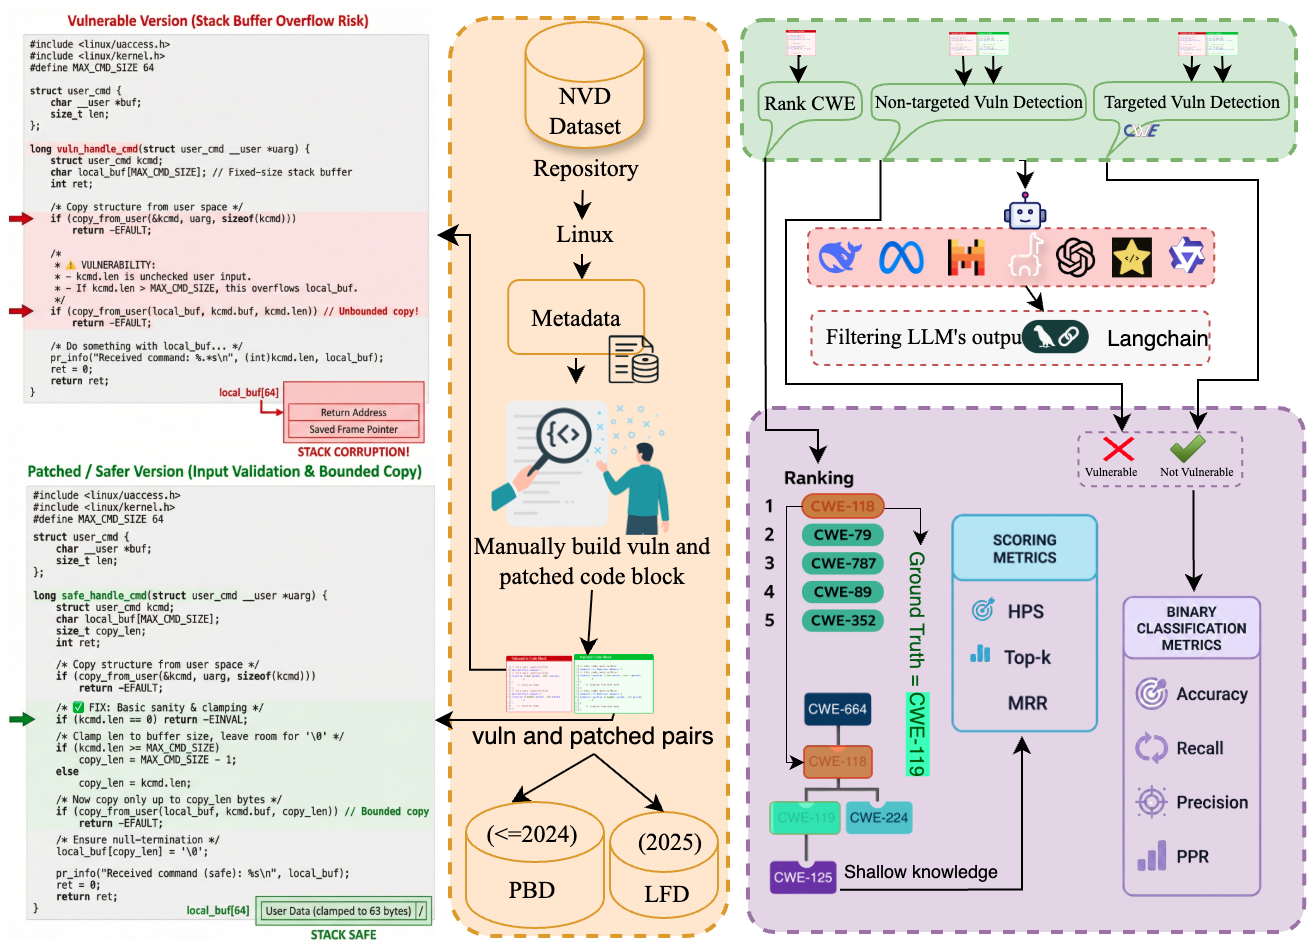
\includegraphics[width=1\textwidth]{figures/LLMKernelBench.png}}
		\caption{LLMKernelBench Framework. Metadata (commit messages, diffs, function/file names) and vulnerable-patched code pairs are extracted from Linux CVE commits. Prompts are designed for \gls{SVD} and CWE-label classification tasks in zero-shot settings. \glspl{LLM} \DIFdelbeginFL \DIFdelFL{performs }\DIFdelendFL \DIFaddbeginFL \DIFaddFL{perform }\DIFaddendFL detection and classification\DIFdelbeginFL \DIFdelFL{. Outputs are filtered via regex. Detection is evaluated using }\DIFdelendFL \DIFaddbeginFL \DIFaddFL{, while LangChain parses raw model outputs and a response audit separates }\DIFaddendFL binary \DIFaddbeginFL \DIFaddFL{verdicts, genuine abstentions, }\DIFaddendFL and \DIFdelbeginFL \DIFdelFL{ranking metrics.}\DIFdelendFL \DIFaddbeginFL \DIFaddFL{invalid outputs}\DIFaddendFL }\DIFaddbeginFL \DIFaddFL{. Detection is evaluated using binary and ranking metrics.
	}\DIFaddendFL \label{figure:framework}
\end{figure*}
\section{Benchmarking Approach}
\label{section:approach}

LLMKernelBench is designed to assess pre-trained \glspl{LLM} (see Table~\ref{table:llm-specs} for the models evaluated) on \gls{SVD} and CWE-label classification tasks, focusing on C code from the Linux kernel while being extensible to other programming languages. As illustrated in Figure\DIFaddbegin \DIFadd{~}\DIFaddend \ref{figure:framework}, the framework is based on vulnerability metadata and code pairs extracted from Linux CVE commits, and includes prompts designed for \gls{SVD} and CWE-label classification tasks. \DIFdelbegin \DIFdel{LLMKernelBench evaluates the models in a zero-shot setting with temperature set to }\DIFdelend \DIFaddbegin \DIFadd{Raw model outputs are processed through the LangChain }\texttt{\DIFadd{VulnerabilityOutputParser}}\DIFadd{; for response-validity analysis, we additionally audit the raw text to distinguish genuine uncertainty from malformed or otherwise non-compliant output. The primary open-source SVD evaluation uses temperature }\DIFaddend 0 \DIFdelbegin \DIFdel{to ensure deterministic and reproducible outputs, using }\DIFdelend \DIFaddbegin \DIFadd{for deterministic decoding. The response-validity sweep averages the two complete temperature-0.1 runs, including GPT-4.1-mini, whereas the CWE-ranking analysis averages its three available ranking runs. We use }\DIFaddend binary classification metrics (precision, recall, accuracy, F1) for \gls{SVD} and ranking metrics for CWE-label classification. This approach ensures benchmark reliability through representativeness (diverse real-world vulnerabilities), adaptability (an extendable methodology), portability (applicability across various \glspl{LLM}), and fairness (standardized evaluation procedures).
\DIFdelbegin %DIFDELCMD < 

%DIFDELCMD < %%%
\DIFdelend Section \ref{section:dataset} details our dataset construction process. Section \ref{section:metrics} defines metrics for \DIFdelbegin \DIFdel{measuring effectiveness in }\DIFdelend \DIFaddbegin \DIFadd{both }\DIFaddend \gls{SVD} and CWE-label classification tasks. Finally, Section \ref{section:prompts} presents our standardized prompt templates.


\subsection{Dataset}
\label{section:dataset}
Our method systematically extracts pairs of vulnerable code blocks and their corresponding patched versions from real-world Linux kernel commits. We focus on the Linux kernel due to its rich vulnerability history and critical security importance. We collect commit hashes, CVE identifiers, and \gls{CWE} classifications from well-known vulnerability databases, including NVD~\cite{nvd2025}, in line with established practices~\cite{pereira2022software}. For each vulnerability-fixing commit, we retrieve the vulnerable code from its parent commit (pre-fix version) and the patched code from the commit itself (post-fix version).

Our extraction process identifies all security-related functions and non-functional elements (global variables, macros, type definitions, structs/unions, headers) that were directly modified in each commit. We include only functions with actual line-level changes, excluding unchanged code to avoid label noise. Non-functional elements are tracked separately as they often form critical vulnerability contexts that influence execution across multiple functions. This comprehensive approach assembles cohesive, vulnerable, and patched code blocks at multiple abstraction levels (single function, multiple functions, multiple files), enabling \glspl{LLM} to analyze complete contextual information rather than isolated fragments.

After extraction, the dataset is divided into two. The \gls{PBD} covers all vulnerabilities discovered on or before 2024, while the \gls{LFD} covers the more recent 2025 vulnerabilities. This division enables us to evaluate the impact of potential data leakage on the model's performance, thereby increasing our confidence in the generalizability of our findings.

\textbf{Manual Review, Denoising, and Deduplication.} Our automated extraction process allowed us to collect a total of 400 samples for PBD and 110 samples for LFD. After that, to ensure dataset integrity and label fidelity, both datasets were manually validated by two different reviewers. For this validation, a standardized protocol that defined inclusion criteria, exclusion criteria, and required evidence documentation was first defined. Then, the original datasets were split in half, and each half was assigned to a different reviewer. The reviewers followed the previously defined documentation to clean the dataset. Doubtful cases were marked for discussion and resolved through consensus sessions between the reviewers. The following validations were performed:

\begin{itemize}
    \item \textbf{Denoising}: Removed samples and functions/files where the changes were not security-related.
    \item \textbf{Completeness check}: Ensured all relevant and security-impacting changes from each commit were included.
    \item \textbf{\gls{CWE} frequency filtering}: CWEs that appeared only once were removed to improve representativeness.
    \item \textbf{Comment removal}: Stripped all code comments from both vulnerable and patched code blocks to eliminate potential biases and ensure that the \glspl{LLM} relied solely on code structure and semantics for \gls{SVD}.
    \item \textbf{Deduplication}: Removed duplicate or near-duplicate code samples (e.g., identical functions, commits, or cloned files) to prevent models from seeing the same or highly similar code during testing.
    \item \textbf{\gls{CWE} labeling}: In the LFD, 40 samples lacked \gls{CWE} identifiers in the NVD database; we manually labeled these samples, strictly adhering to NVD criteria for consistent labeling.
\end{itemize}

Table~\ref{table:dataset-stats} summarizes the overall size and composition of the \gls{PBD} and \gls{LFD} after this comprehensive cleaning process. The final \gls{PBD} dataset comprises \DIFdelbegin \DIFdel{a total of }\DIFdelend 314 samples \DIFdelbegin \DIFdel{and spans }\DIFdelend \DIFaddbegin \DIFadd{spanning }\DIFaddend 74 \DIFdelbegin \DIFdel{different }\DIFdelend \DIFaddbegin \DIFadd{distinct }\DIFaddend CWEs, while the final \gls{LFD} \DIFaddbegin \DIFadd{dataset }\DIFaddend contains 103 samples belonging to 19 \DIFdelbegin \DIFdel{different }\DIFdelend CWEs.

%The fundamental approach of LLMKernelBench assembles all touched functions and non-functional elements (macros, libraries, type definitions) into cohesive vulnerable and patched code blocks that \glspl{LLM} can comprehensively analyze for vulnerability prediction, ensuring complete contextual understanding rather than isolated code fragment analysis.

%Initially, we collected 400 samples for PBD and 110 samples for LFD through our automated extraction process. To ensure dataset integrity and label fidelity, both datasets underwent rigorous quality control through a structured two-author review process. Two authors independently evaluated every sample using a standardized protocol that defined inclusion criteria (security-relevant commits with confirmed CVE identifiers, function-level line modifications, and extractable vulnerable-patched pairs), exclusion criteria (cosmetic refactoring, formatting-only changes, test modifications, and commits lacking substantiated security relevance), and required evidence documentation (CVE/\gls{CWE} identifiers, commit metadata, and security rationale). Each reviewer assigned decision labels (Keep, Exclude, Requires-Discussion) with documented reasoning codes to ensure traceability and reproducibility. Inter-reviewer agreement was measured using Cohen's kappa, and all disagreements were resolved through consensus sessions with explicit rationale recording. Systematic denoising removed samples and touched functions/files that were not security-related, eliminating non-functional changes while preserving essential contextual elements necessary for semantic correctness. We removed singleton CWEs (vulnerabilities appearing only once) to ensure statistical reliability and prevent overrepresentation of rare, potentially outlier cases that could skew model evaluation. Additionally, we stripped all code comments from both vulnerable and patched code blocks to eliminate potential biases that could arise from human annotations, ensuring LLMs rely solely on code structure and semantics for VD. Deduplication removed duplicate or near-duplicate code samples (e.g., identical functions, commits, or cloned files) to prevent models from seeing the same or highly similar code during testing, employing both exact hash-based matching and token-level similarity metrics with manual inspection of flagged candidates to ensure canonical representation. Each dataset contained only one multi-label \gls{CWE} vulnerability, which we retained with comprehensive annotations rather than creating duplicate entries. For LFD, we manually labeled 40 samples that lacked \gls{CWE} identifiers in the NVD database, strictly adhering to NVD criteria for consistent labeling. After this comprehensive cleaning process, our final datasets comprised 314 samples in PBD and 103 samples in LFD. The fundamental approach of LLMKernelBench assembles all touched functions and non-functional elements (macros, libraries, type definitions) into cohesive vulnerable and patched code blocks that LLMs can comprehensively analyze for vulnerability prediction, ensuring complete contextual understanding rather than isolated code fragment analysis.

\textbf{\gls{CWE} Distribution and Label Space.} \DIFaddbegin \DIFadd{We did not pre-select a preferred subset of CWEs. PBD retains the CWE labels associated with the sampled Linux-kernel CVEs, while 40 LFD samples lacking NVD CWE identifiers were manually labeled under NVD-aligned criteria. The resulting label space, spanning 74 distinct CWEs in PBD and 19 in LFD, therefore reflects the sampled kernel vulnerabilities rather than an artificially balanced category design. }\DIFaddend Our dataset spans diverse \gls{CWE} categories organized according to the CWE-1000 hierarchical view \cite{cwe1000}. Table~\ref{table:cwe-pillars-combined} \DIFdelbegin \DIFdel{shows the distribution of vulnerabilities across the }\DIFdelend \DIFaddbegin \DIFadd{reports coverage against the }\DIFaddend ten fundamental \gls{CWE} pillars\DIFdelbegin \DIFdel{in PBD}\DIFdelend \DIFaddbegin \DIFadd{: eight have nonzero coverage in the sampled data, while deprecated or otherwise unmapped labels are grouped as CWE-OTHER}\DIFaddend . CWE-664 accounts for 43.3\% of \DIFaddbegin \DIFadd{PBD }\DIFaddend coverage, reflecting the prevalence of memory-related vulnerabilities in the Linux kernel. The distribution also includes 12.1\% deprecated \gls{CWE} identifiers (CWE-OTHER), representing historical vulnerability classifications that MITRE now marks as \enquote{PROHIBITED} for mapping.
\DIFdelbegin \DIFdel{This diverse distribution ensures comprehensive evaluation across different security weakness categories, from common memory safety issues to rare configuration vulnerabilities.
}\DIFdelend 

\begin{table}[!t]
\centering
\caption{LLMKernelBench dataset statistics}
\label{table:dataset-stats}
\scriptsize
\setlength{\tabcolsep}{22pt}
\renewcommand{\arraystretch}{1.1}
\resizebox{\columnwidth}{!}{%
\begin{tabular}{@{}lrr@{}}
\toprule
\textbf{Metric} & \textbf{PBD} & \textbf{LFD} \\
\midrule
Vulnerabilities & 314 & 103 \\
Unique CWEs & 74 & 19 \\
\cmidrule(lr){1-3}
Files/Functions Changed (avg) & 1.5 / 2.0 & 1.1 / 1.3 \\
Vuln/Patched Lines (avg) & 109.4 / 114.1 & 60.9 / 63.6 \\
Lines Added/Deleted (avg) & 17.6 / 9.0 & 7.0 / 3.5 \\
\bottomrule
\end{tabular}
}
\end{table}




\begin{comment}
    \begin{table}[!t]
\centering
\caption{\gls{CWE} Pillar Distribution in PBD}
\label{table:cwe-pillars}
\renewcommand{\arraystretch}{1.1}
\small
\resizebox{\columnwidth}{!}{%
\begin{tabular}{@{}llcc@{}}
\toprule
\textbf{CWE-ID} & \textbf{Pillar Name} & \textbf{Coverage (\%)} \\
\midrule
CWE-664 & Improper Control of Resource Lifetime & 136 (43.3) \\
CWE-OTHER & Other/Unmapped CWEs & 12.1 \\
CWE-682 & Incorrect Calculation & 10.2 \\
CWE-284 & Improper Access Control & 8.9 \\
CWE-691 & Insufficient Control Flow Management & 8.6 \\
CWE-707 & Improper Neutralization & 5.7 \\
CWE-693 & Protection Mechanism Failure & 5.1 \\
CWE-710 & Improper Adherence to Coding Standards & 3.5 \\
CWE-703 & Improper Check/Handling of Except. Conditions & 2.9 \\
CWE-435 & Improper Interaction Between Components & 0.0 \\
CWE-697 & Incorrect Comparison & 0.0 \\
\bottomrule
\end{tabular}%
}
\vspace{-4pt}
\end{table}
\end{comment}





\begin{table}[!t]
\centering
\caption{\gls{CWE} pillar distribution across PBD and LFD.}
\label{table:cwe-pillars-combined}
\small
\renewcommand{\arraystretch}{1.1}
\resizebox{\columnwidth}{!}{%
\begin{tabular}{@{}llcc@{}}
\toprule
\textbf{CWE-ID} & \textbf{Pillar Name} & \multicolumn{2}{c}{\textbf{Coverage} (\%)} \\ 
\cmidrule(lr){3-4}
& & \textbf{PBD} & \textbf{LFD} \\
\midrule
CWE-664 & Improper Control of Resource Lifetime & 136 (43.3) & 62 (60.2) \\
CWE-OTHER & Other/Unmapped CWEs & 38 (12.1) & 0 (0.0) \\
CWE-682 & Incorrect Calculation & 32 (10.2) & 7 (6.8) \\
CWE-284 & Improper Access Control & 28 (8.9) & 0 (0.0) \\
CWE-691 & Insufficient Control Flow Management & 27 (8.6) & 11 (10.7) \\
CWE-707 & Improper Neutralization & 18 (5.7) & 9 (8.7) \\
CWE-693 & Protection Mechanism Failure & 16 (5.1) & 0 (0.0) \\
CWE-710 & Improper Adherence to Coding Standards & 11 (3.5) & 14 (13.6) \\
CWE-703 & Improper Check/Handling of Except. Conditions & 9 (2.9) & 0 (0.0) \\
CWE-435 & Improper Interaction Between Components & 0 (0.0) & 0 (0.0) \\
CWE-697 & Incorrect Comparison & 0 (0.0) & 0 (0.0) \\
\bottomrule
\end{tabular}%
}
\end{table}


\subsection{Tasks}
\label{section:tasks}

Based on this dataset, the models are evaluated across two different tasks: \gls{SVD} and vulnerability type identification.

\textbf{\gls{SVD}}. In this task, the models are given either a vulnerable code block (pre-fix versions from parent commits) or a non-vulnerable (patched) code block (post-fix versions from fixing commits). They are then asked to classify the code block as vulnerable (\DIFdelbegin \DIFdel{1}\DIFdelend \DIFaddbegin \texttt{\DIFadd{1}}\DIFaddend ), non-vulnerable (\DIFdelbegin \DIFdel{0}\DIFdelend \DIFaddbegin \texttt{\DIFadd{0}}\DIFaddend ), or to \DIFdelbegin \DIFdel{abstain from classifying it (-1). }\DIFdelend \DIFaddbegin \DIFadd{answer }\texttt{\DIFadd{not sure}}\DIFadd{. The uncertainty response is represented as $-1$ in the structured evaluation data. }\DIFaddend This third option is used because: (1) real-world \gls{SVD} often involves ambiguous cases where even security experts disagree; (2) it prevents \glspl{LLM} from making forced binary decisions when evidence is insufficient, potentially reducing false positives and negatives; and (3) it mirrors practical security analysis workflows where analysts may need to flag code for further investigation rather than making definitive vulnerability determinations. 

%It is important to note that, for all binary \gls{SVD}/\gls{SPV} tasks (SVD3--SVD6), we use labels $y\in\{1,0\}$, where $y=1$ denotes \emph{vulnerable} code (the pre-fix version from the parent commit) and $y=0$ denotes \emph{patched} code (the post-fix version from the fixing commit). During inference we allow models to abstain with $-1$ (\enquote{not sure}); this is an optional prediction class and \emph{not} a ground-truth label.

\textbf{CWE-label classification.} The \gls{CWE} taxonomy organizes weaknesses into a hierarchical structure with four abstraction levels as shown in Figure~\ref{fig:cwe_hierarchy}: \textit{Pillars} (highest level, 10 fundamental categories representing root security principles such as CWE-664 Improper Control of a Resource Through its Lifetime), \textit{Classes} (general weakness types like CWE-119 Buffer Errors), \textit{Bases} (specific weakness variants such as CWE-120 Buffer Copy without Checking Size of Input), and \textit{Variants} (detailed platform-specific manifestations). This hierarchy is formalized in the CWE-1000 Research Concepts view~\cite{cwe1000}.
% \begin{figure*}
%     \centering
%     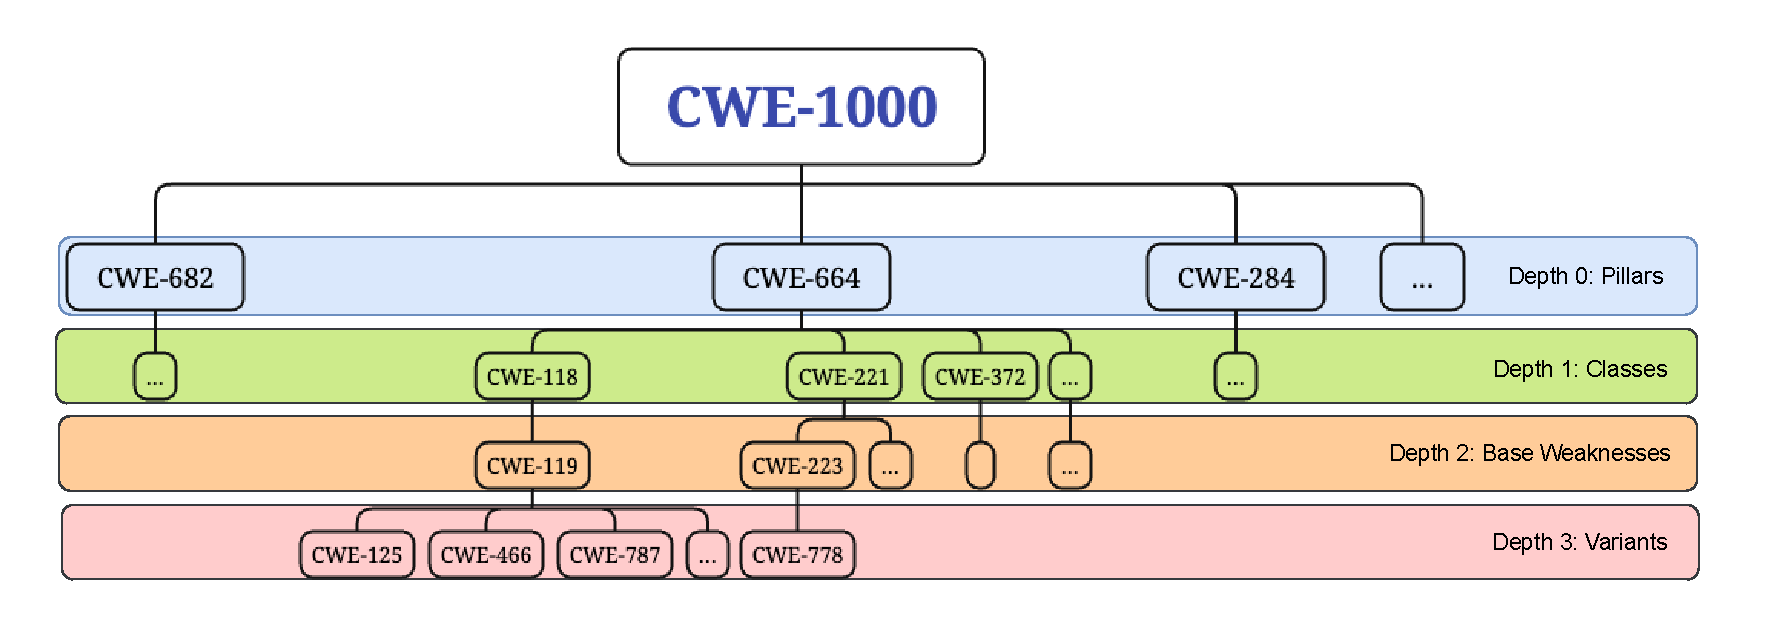
\includegraphics[width=0.8\textwidth]{figures/cwe_hierarchy.pdf}
%     \caption{CWE hierarchy}
%     \label{fig:cwe_hierarchy}
% \end{figure*}

\begin{figure}[h]
    \centering
    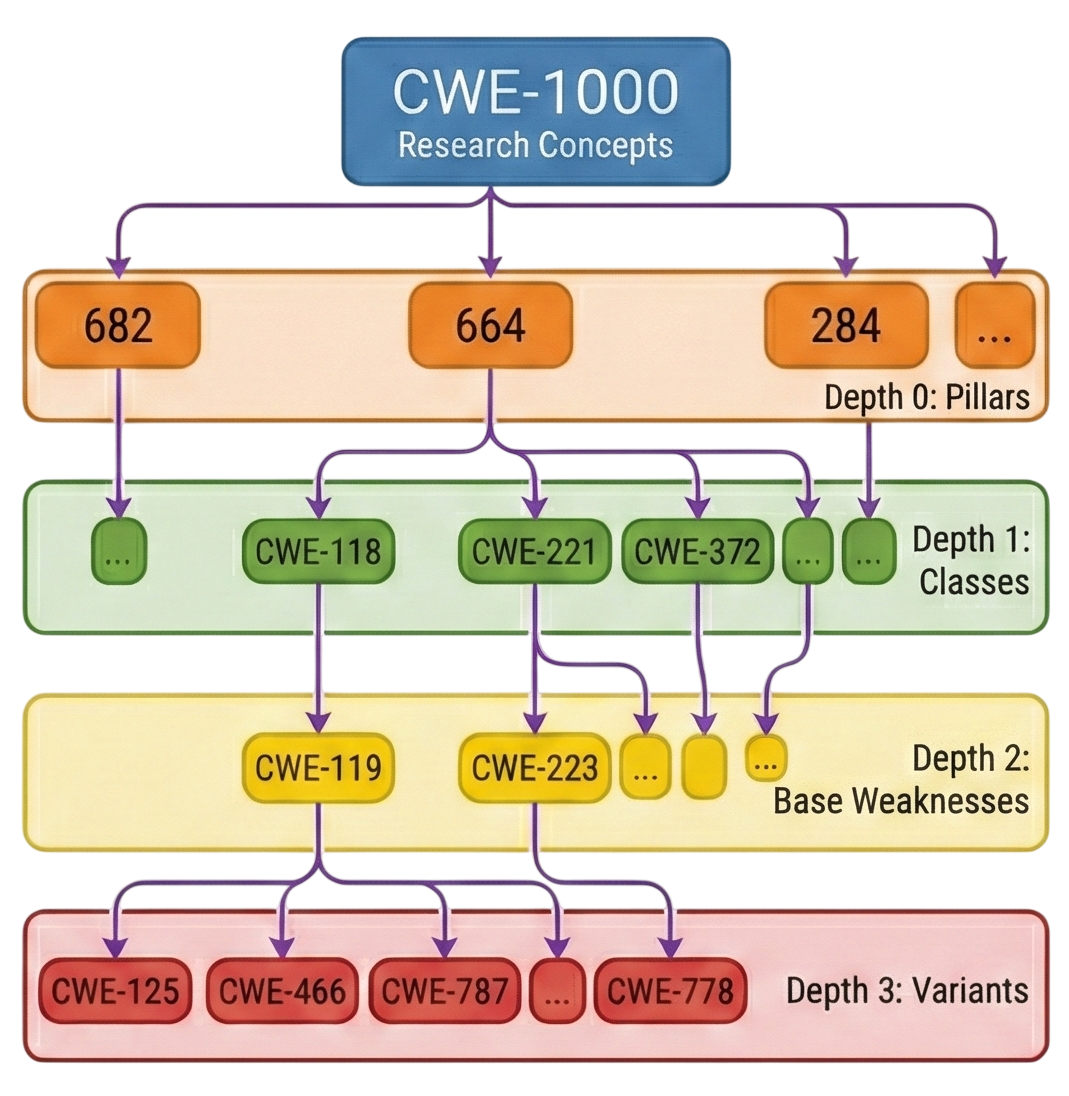
\includegraphics[width=0.8\columnwidth]{figures/cwe_hierarchy.png}
    \caption{CWE hierarchy.}
    \label{fig:cwe_hierarchy}
\end{figure}

For our \gls{CWE} classification tasks, we employ a \textit{hierarchical evaluation approach} that assesses model predictions across all \DIFdelbegin \DIFdel{abstraction }\DIFdelend \DIFaddbegin \DIFadd{taxonomy }\DIFaddend levels rather than focusing solely on exact matches.
This design \DIFdelbegin \DIFdel{enables us to measure the }\textit{\DIFdel{depth of security knowledge}} %DIFAUXCMD
\DIFdel{exhibited by \mbox{%DIFAUXCMD
\glspl{LLM}}\hskip0pt%DIFAUXCMD
, distinguishing between models that demonstrate only shallow, }\DIFdelend \DIFaddbegin \DIFadd{measures the taxonomic proximity of model outputs, distinguishing broad }\DIFaddend category-level \DIFdelbegin \DIFdel{understanding (e.g., correctly identifying a vulnerability as }%DIFDELCMD < \enquote{resource management} %%%
\DIFdel{but unable to specify the exact type) versus those with deep, }\DIFdelend \DIFaddbegin \DIFadd{matches from exact }\DIFaddend fine-grained \DIFdelbegin \DIFdel{comprehension (e.g., pinpointing CWE-772 Missing Release of Resource after Effective Lifetime)}\DIFdelend \DIFaddbegin \DIFadd{identification without assuming that proximity alone demonstrates semantic understanding}\DIFaddend .

We introduce the \gls{HPS} metric (\S\ref{section:metrics}), which \DIFdelbegin \DIFdel{quantifies how hierarchically close a predicted \mbox{%DIFAUXCMD
\gls{CWE} }\hskip0pt%DIFAUXCMD
is to the true label by computing path distance }\DIFdelend \DIFaddbegin \DIFadd{assigns ordinal credit according to exact, immediate parent/child, sibling, same-root, or unrelated relations }\DIFaddend in the CWE-1000 \DIFdelbegin \DIFdel{taxonomy tree}\DIFdelend \DIFaddbegin \DIFadd{hierarchy}\DIFaddend .
A prediction of \DIFdelbegin \DIFdel{CWE-119 (Buffer Errors, Class level}\DIFdelend \DIFaddbegin \DIFadd{CWE-121 (Stack-based Buffer Overflow}\DIFaddend ) when the true answer is \DIFdelbegin \DIFdel{CWE-121 (Stack-based Buffer Overflow, Base level}\DIFdelend \DIFaddbegin \DIFadd{CWE-787 (Out-of-bounds Write}\DIFaddend ) receives partial \DIFdelbegin \DIFdel{credit, as it demonstrates understanding of the vulnerability family }\DIFdelend \DIFaddbegin \DIFadd{child credit, recording a related candidate }\DIFaddend despite missing the \DIFdelbegin \DIFdel{specific subtype}\DIFdelend \DIFaddbegin \DIFadd{exact type}\DIFaddend .
This approach addresses practical challenges in \gls{CWE} classification: fine-grained labels (bases and variants) exhibit severe class imbalance, with many specific types having fewer than 10 examples in real-world datasets, rendering exact-match accuracy unreliable.
Meanwhile, coarse-grained evaluation at only the pillar level (10 categories) would be too lenient \DIFdelbegin \DIFdel{, failing to distinguish between models that truly understand security concepts versus those that merely memorize broad categories}\DIFdelend \DIFaddbegin \DIFadd{to distinguish precise weakness identification from broad category prediction}\DIFaddend .

Our hierarchical scoring thus \DIFdelbegin \DIFdel{captures a spectrum of understanding: models achieving high }\DIFdelend \DIFaddbegin \DIFadd{separates exact }\DIFaddend Top-1 \DIFdelbegin \DIFdel{accuracy (i.e., the model's first prediction is the correct label; defined in \S\ref{section:cwe_metrics}) demonstrate precise knowledge of specific vulnerability types, while those with high \mbox{%DIFAUXCMD
\gls{HPS} }\hskip0pt%DIFAUXCMD
but }\DIFdelend \DIFaddbegin \DIFadd{identification from taxonomically related candidate output. High HPS with }\DIFaddend low Top-1 accuracy \DIFdelbegin \DIFdel{reveal }\DIFdelend \DIFaddbegin \DIFadd{indicates related labels in the candidate set, not necessarily }\DIFaddend taxonomy-aware reasoning\DIFdelbegin \DIFdel{, correctly identifying the vulnerability family but struggling with fine-grained distinctions}\DIFdelend .
This multi-level evaluation \DIFdelbegin \DIFdel{provides actionable insights for both model developers (to identify where models need improvement) and security practitioners (to understand whether a model's predictions are reliable enough for specific use cases)}\DIFdelend \DIFaddbegin \DIFadd{helps model developers locate error patterns and helps practitioners judge whether candidate labels are suitable only for routing or are accurate enough for diagnosis}\DIFaddend .

By considering both these tasks, our benchmark systematically evaluates \glspl{LLM} in terms of their ability to (1) detect the presence of vulnerabilities through binary \gls{SVD} classification, and (2) identify and prioritize the most likely underlying vulnerability types through \gls{CWE}-label ranking.

\subsection{Metrics}
\label{section:metrics}

Due to the different nature of the two tasks, different metrics must be employed. These metrics, along with statistical significance testing, are discussed next. 

\subsubsection{SVD}

To evaluate the models' performance at \gls{SVD}, we consider the following terms: \gls{TP} refers to the number of vulnerable code samples that the model correctly identifies as vulnerable; \gls{FP} is the number of non-vulnerable samples incorrectly predicted as vulnerable; \gls{TN} represents the number of non-vulnerable samples correctly classified as non-vulnerable; while \gls{FN} represents the number of vulnerable samples that the model fails to identify, incorrectly classifying them as non-vulnerable. These four quantities form the basis for calculating the performance metrics described below.

It is important to note that these metrics are computed only for cases in which the models \DIFdelbegin \DIFdel{actually provided a }\DIFdelend \DIFaddbegin \DIFadd{provided a valid binary }\DIFaddend classification, i.e., \DIFdelbegin \DIFdel{when they predicted either vulnerable (1}\DIFdelend \DIFaddbegin \DIFadd{vulnerable (}\texttt{\DIFadd{1}}\DIFaddend ) or non-vulnerable (\DIFdelbegin \DIFdel{0). Samples for which the models abstained from answering (returning }\texttt{\DIFdel{-1}}%DIFAUXCMD
\DIFdel{) are excludedfrom these metric calculations. In addition to reporting the standard metrics, we also provide a breakdown of how frequently each model responded versus abstained. This distinction is critical for a fair interpretation of the results (e.g., a high recall when a model only classified 5\% of the samples does not carry the same significance as when it classifies 90\% of the inputs). }\DIFdelend \DIFaddbegin \texttt{\DIFadd{0}}\DIFadd{). Genuine abstentions and invalid outputs are excluded. We distinguish these outcomes by auditing the raw response: a }\emph{\DIFadd{genuine abstention}} \DIFadd{clearly selects }\texttt{\DIFadd{not sure}} \DIFadd{(either alone or as an unambiguous final verdict motivated by insufficient information), whereas an }\emph{\DIFadd{invalid response}} \DIFadd{does not yield a single resolvable verdict, for example because it continues the input code, loops, or presents contradictory choices. Reporting these categories separately is critical because parser failure or prompt non-compliance should not be interpreted as model uncertainty. }\DIFaddend The following metrics are used:

\begin{itemize}
    \item \textbf{Accuracy}: measures the proportion of correctly classified code samples among all samples:

    \begin{equation}
    \text{Accuracy} = \frac{TP+TN}{TP+FP+TN+FN}
    \end{equation}

    As the dataset is relatively balanced between vulnerable and non-vulnerable samples, the accuracy accurately reflects the model’s overall performance without being dominated by one class. High accuracy is important as it indicates that the model performs well across both classes.

    \item \textbf{Recall} – measures the proportion of actual vulnerable code samples that were correctly identified by the model:

    \begin{equation}
        \text{Recall} = \frac{TP}{TP+FN}
    \end{equation}

    In this context, it represents the number of true vulnerabilities the \gls{LLM} successfully detects or flags. High recall is crucial, as missing vulnerable samples could lead to the overlooking of potential security issues.

    \item \textbf{Precision} – measures the proportion of code samples predicted as vulnerable that are truly vulnerable: 

    \begin{equation}
        \text{Precision} = \frac{TP}{TP+FP}
    \end{equation}

    This metric indicates how many of the flagged samples are genuine vulnerabilities rather than false positives. High precision is important to reduce the number of incorrect alerts, which can waste time during manual inspection or downstream analysis.

    \item \textbf{\gls{PPR}} – measures the proportion of all samples that the model classifies as vulnerable, regardless of correctness:

    \begin{equation}
    \text{PPR} = \frac{TP+FP}{TP+FP+TN+FN}
    \end{equation}

    While this metric is not as critical as precision or recall, it provides valuable insight into the model’s potential bias toward one class. A higher PPR may indicate a tendency to over-predict vulnerabilities, whereas a lower PPR suggests under-prediction. Comparing the PPR across models helps identify whether a model systematically favors one class over the other, offering additional context for interpreting performance results.

\end{itemize}

Together, these metrics provide a comprehensive evaluation of classification performance, balancing correctness, sensitivity, and class bias.

\subsubsection{CWE-label classification}
\label{section:cwe_metrics}
For the task of CWE-label classification, the following metrics are employed:

\begin{itemize}

	\item \textbf{Top-k Accuracy}~\cite{russakovsky2015imagenet}: Considers a prediction correct if the true vulnerability type appears among the model's k highest-ranked predictions. We measure Top-1 to Top-5 accuracy to evaluate how well models detect and rank both CVEs and CWEs. This progressive evaluation is particularly valuable in security contexts where identifying the correct vulnerability category among top candidates enables more efficient remediation efforts, even when exact classification is challenging.

	\item \textbf{\DIFdelbegin \DIFdel{\mbox{%DIFAUXCMD
\gls{MMR}}\hskip0pt%DIFAUXCMD
}\DIFdelend \DIFaddbegin \DIFadd{\mbox{%DIFAUXCMD
\gls{MRR}}\hskip0pt%DIFAUXCMD
}\DIFaddend }~\cite{craswell2009mean}: Evaluates ranking quality by calculating:

    \begin{equation}
        \frac{1}{N}\sum_{i=1}^{N}\frac{1}{\text{rank}_i}
    \end{equation}

    Where $\text{rank}_i$ is the position of the correct answer in the ranked list for the $i$-th query. MRR rewards models that rank the correct vulnerability type higher, recognizing that, in security contexts, prioritizing findings is crucial.

    \item \textbf{\gls{HPS}} scores a model's outputs by how close they are to the ground-truth \gls{CWE} in the hierarchy. We assign weights: $\text{exact}=1.0$, $\text{parent}=0.8$, $\text{child}=0.7$, $\text{sibling}=0.6$, $\text{same-root}=0.4$, $\text{unrelated}=0.0$. \DIFaddbegin \DIFadd{CWE-1000 is a directed acyclic graph rather than a strict tree because a weakness may have multiple parents or occur under multiple pillars. Parent and child therefore denote any immediate taxonomy edge, siblings share at least one immediate parent, and same-root labels share at least one top-level pillar. }\DIFaddend The HPS weighting scheme follows an ordinal decay aligned with the CWE hierarchy rather than modeling precise semantic distances. Higher weights reflect closer ancestry in the taxonomy, as confusing a vulnerability with \DIFdelbegin \DIFdel{a }\DIFdelend \DIFaddbegin \DIFadd{an immediate }\DIFaddend parent or child category indicates greater \DIFdelbegin \DIFdel{understanding }\DIFdelend \DIFaddbegin \DIFadd{taxonomic proximity }\DIFaddend than predicting an unrelated weakness. The specific values \DIFdelbegin \DIFdel{are intended to }\DIFdelend preserve hierarchical ordering and distinguish near-misses from \DIFdelbegin \DIFdel{random errors, not to encode exact }\DIFdelend \DIFaddbegin \DIFadd{unrelated predictions; they do not encode calibrated }\DIFaddend semantic margins. Formally, let \DIFdelbegin \DIFdel{$y_i$ be the ground truth and $(\hat y_{i1},\dots,\hat y_{ik})$ the top-$k$ predictions}\DIFdelend \DIFaddbegin \DIFadd{$Y_i$ be the set of ground-truth labels and $(\hat y_{i1},\dots,\hat y_{ik_i})$ the valid predicted labels}\DIFaddend . Define $r(\hat y,y)\in\{\text{exact},\text{parent},\text{child},\text{sibling},\text{root},\text{none}\}$ and a weight map $w(\cdot)$ as above. \DIFdelbegin \DIFdel{The per-sample score is
    }\DIFdelend \DIFaddbegin \DIFadd{Each predicted label receives its best score against the ground-truth set,
    }\DIFaddend 

    \begin{equation}
      \DIFdelbegin \DIFdel{\mathrm{HPS}_i}\DIFdelend \DIFaddbegin \DIFadd{s_{ij}}\DIFaddend =\max\DIFdelbegin \DIFdel{_{1\le j\le k} }\DIFdelend \DIFaddbegin \DIFadd{_{y\in Y_i} }\DIFaddend w\big(r(\hat y_{ij},y\DIFdelbegin \DIFdel{_i}\DIFdelend )\big),
    \end{equation}

    and the \DIFdelbegin \DIFdel{dataset score is $\mathrm{HPS}=\tfrac{1}{N}\sum_{i=1}^N \mathrm{HPS}_i$. \mbox{%DIFAUXCMD
\gls{HPS}  }\hskip0pt%DIFAUXCMD
credits near-misses that are semantically related, which is useful for prioritization in security triage}\DIFdelend \DIFaddbegin \DIFadd{implemented dataset score averages across all valid predicted labels,
    }\begin{equation}
      \DIFadd{\mathrm{HPS}=\frac{\sum_i\sum_{j=1}^{k_i}s_{ij}}{\sum_i k_i}.
    }\end{equation}
    \DIFadd{Thus HPS measures taxonomic proximity of the candidate set, while Top-$k$ accuracy and MRR separately measure exact inclusion and rank. For the supporting distance audit in Tables~\ref{tab:hps_validation_stats} and~\ref{tab:hierarchy_distance_dist}, distance is the shortest path in the undirected CWE-1000 parent--child graph. We connect the ten top-level pillars through a virtual root so that cross-pillar errors have finite distances; unmapped or deprecated identifiers remain unmeasurable. The committed HPS and distance-analysis scripts preserve all parent and pillar memberships and regenerate the reported values directly from the three ranking runs.
}

    \DIFadd{To ground this metric in a practical security context, consider a true CWE-787 (Out-of-bounds Write) with a predicted CWE-121 (Stack-based Buffer Overflow). CWE-121 is an immediate child of CWE-787 in the benchmark hierarchy and therefore receives the child weight of 0.7. By contrast, CWE-284 (Improper Access Control) is in a different root branch and receives 0.0. In SOC triage, the former can still route an alert toward buffer-handling review, but it must not be treated as an exact diagnosis}\DIFaddend .

\end{itemize}

By combining these metrics, we \DIFdelbegin \DIFdel{obtain a holistic view of model performance, capturing not only classification accuracyand ranking qualitybut also the semantic }\DIFdelend \DIFaddbegin \DIFadd{evaluate classification accuracy, ranking quality, and the taxonomic }\DIFaddend proximity of predicted vulnerability categories.


\subsubsection{Statistical Significance Testing}
To \DIFdelbegin \DIFdel{determine whether observed performance differences across experimental conditions }\DIFdelend \DIFaddbegin \DIFadd{assess whether performance differences }\DIFaddend are statistically meaningful \DIFdelbegin \DIFdel{or merely due to randomvariation, we employ three complementary statistical approaches: statistical tests for }\DIFdelend \DIFaddbegin \DIFadd{rather than random, we combine }\DIFaddend group-level \DIFdelbegin \DIFdel{differences}\DIFdelend \DIFaddbegin \DIFadd{tests}\DIFaddend , degradation metrics\DIFdelbegin \DIFdel{to quantify performance changes across abstraction levels, and Pearson correlation to assess relationships between continuous variables (e.g., context window size and model degradation)}\DIFdelend \DIFaddbegin \DIFadd{, and correlation analysis}\DIFaddend .

\DIFdelbegin %DIFDELCMD < \begin{itemize}
%DIFDELCMD <     \item %%%
\DIFdelend \textbf{Statistical \DIFdelbegin \DIFdel{Test Selection}%DIFDELCMD < \MBLOCKRIGHTBRACE%%%
\DIFdel{: To compare model performance across three }\DIFdelend \DIFaddbegin \DIFadd{test selection.}} \DIFadd{To compare accuracy across }\DIFaddend abstraction levels (\DIFdelbegin \DIFdel{L1, L2, L3}\DIFdelend \DIFaddbegin \DIFadd{L1--L3}\DIFaddend ), we \DIFdelbegin \DIFdel{follow a systematic approach to select the appropriate statistical test. First, we validate normality using the }\DIFdelend \DIFaddbegin \DIFadd{first check normality (}\DIFaddend Shapiro-Wilk\DIFdelbegin \DIFdel{\mbox{%DIFAUXCMD
\cite{shapiro1965analysis} }\hskip0pt%DIFAUXCMD
test for each group. Second, we test }\DIFdelend \DIFaddbegin \DIFadd{~\mbox{%DIFAUXCMD
\cite{shapiro1965analysis}}\hskip0pt%DIFAUXCMD
) and }\DIFaddend homogeneity of variance \DIFdelbegin \DIFdel{using Levene's test. If both assumptions hold, we use }\DIFdelend \DIFaddbegin \DIFadd{(Levene). We then apply }\DIFaddend one-way ANOVA\DIFdelbegin \DIFdel{(parametric) \mbox{%DIFAUXCMD
\cite{fisher1970statistical} }\hskip0pt%DIFAUXCMD
; if only normality holds but variances differ, we use }\DIFdelend \DIFaddbegin \DIFadd{~\mbox{%DIFAUXCMD
\cite{fisher1970statistical} }\hskip0pt%DIFAUXCMD
when both hold, }\DIFaddend Welch's ANOVA \DIFdelbegin \DIFdel{; if normality fails, we use the }\DIFdelend \DIFaddbegin \DIFadd{when variances differ, and the non-parametric }\DIFaddend Kruskal-Wallis H-test \DIFdelbegin \DIFdel{(non-parametric alternative). For PBD , all groups pass normality (Shapiro-Wilk p$>$0.05) and equal variance tests (}\DIFdelend \DIFaddbegin \DIFadd{when normality fails. PBD satisfies both assumptions (}\DIFaddend Levene p=0.812), justifying \DIFdelbegin \DIFdel{one-way ANOVA. For LFD, Level }\DIFdelend \DIFaddbegin \DIFadd{ANOVA, whereas LFD Level~}\DIFaddend 3 fails normality (p=0.008) \DIFdelbegin \DIFdel{, requiring the }\DIFdelend \DIFaddbegin \DIFadd{and uses }\DIFaddend Kruskal-Wallis\DIFdelbegin \DIFdel{test. Both tests evaluate whether abstraction level significantly affects accuracy, with }\DIFdelend \DIFaddbegin \DIFadd{; }\DIFaddend p$<$0.05 \DIFdelbegin \DIFdel{indicating significant differences and p$\geq$0.05 suggesting no meaningful effect beyond random variation}\DIFdelend \DIFaddbegin \DIFadd{denotes a significant effect of abstraction level on accuracy}\DIFaddend .

\DIFdelbegin %DIFDELCMD < \item %%%
\DIFdelend \textbf{Degradation} \DIFdelbegin \DIFdel{: Measures the change in model accuracy across abstraction levels, calculated as $\text{Degradation} = \text{Accuracy}_{\text{L1}} - \text{Accuracy}_{\text{L3}}$. Positive degradation values indicate performance decline as code scopeincreases (higher abstraction levels), while negative values indicate improvementwith broader context. This metric quantifies model robustness to code abstraction: models with }\DIFdelend \DIFaddbegin \DIFadd{quantifies robustness to context as $\text{Accuracy}_{\text{L1}}-\text{Accuracy}_{\text{L3}}$: positive values denote decline with broader scope, negative values improvement, and }\DIFaddend near-zero \DIFdelbegin \DIFdel{degradation maintain stable performance regardless of abstraction level, while high degradation reveals fragility when processing multi-file scenarios versus isolated functions}\DIFdelend \DIFaddbegin \DIFadd{values stable behavior across levels}\DIFaddend .

\DIFdelbegin %DIFDELCMD < \item %%%
\DIFdelend \textbf{Pearson \DIFdelbegin \DIFdel{Correlation}\DIFdelend \DIFaddbegin \DIFadd{correlation}\DIFaddend } \DIFdelbegin \DIFdel{: Measures }\DIFdelend \DIFaddbegin \DIFadd{($r\in[-1,1]$) measures }\DIFaddend the strength and direction of \DIFdelbegin \DIFdel{linear relationships between two }\DIFdelend \DIFaddbegin \DIFadd{the linear relationship between two continuous }\DIFaddend variables (e.g., context window size \DIFdelbegin \DIFdel{and model degradation). The correlation coefficient (r) ranges from -1 to +1, where values close to 0 indicate no linear relationship, while values near $\pm$1 indicate strong positive or negative correlation. Statistical significance is assessed via }\DIFdelend \DIFaddbegin \DIFadd{vs.\ degradation), with significance assessed via its }\DIFaddend p-value\DIFdelbegin \DIFdel{, where p$<$0.05 indicates the correlation is unlikely due to chance}\DIFdelend .

\DIFdelbegin %DIFDELCMD < \item %%%
\DIFdelend \textbf{Mann-Whitney U\DIFdelbegin \DIFdel{Test}\DIFdelend }~\cite{mann1947test} \DIFdelbegin \DIFdel{: A }\DIFdelend \DIFaddbegin \DIFadd{is a }\DIFaddend non-parametric\DIFdelbegin \DIFdel{statistical test used to compare }\DIFdelend \DIFaddbegin \DIFadd{, rank-based test for }\DIFaddend two independent groups \DIFdelbegin \DIFdel{when data do not meet the assumptions required for parametric tests (e.g., t-test). Unlike the t-test, which assumes normally distributed data with equal variances, the Mann-Whitney U test operates on ranked data and }\DIFdelend \DIFaddbegin \DIFadd{that }\DIFaddend is robust to outliers and skewed \DIFdelbegin \DIFdel{distributions. The test works by ranking all observations from both groups together, then comparing the sum of ranks between groups. The U statistic represents the number of times observations from one group precede observations from the other group in the ranking. For our abstraction level analysis, we use Mann-Whitney U }\DIFdelend \DIFaddbegin \DIFadd{or unequal-sized samples. We use it }\DIFaddend to compare Simple (L1) versus Complex (L2+L3) \DIFdelbegin \DIFdel{categories }\DIFdelend \DIFaddbegin \DIFadd{accuracy }\DIFaddend in LFD, where the small \DIFdelbegin \DIFdel{sample size for }\DIFdelend L3 \DIFaddbegin \DIFadd{sample }\DIFaddend (n=3) \DIFdelbegin \DIFdel{violates normality assumptions and creates highly unequal group sizes }\DIFdelend \DIFaddbegin \DIFadd{and group imbalance }\DIFaddend (85 vs\DIFaddbegin \DIFadd{.\ }\DIFaddend 18) \DIFdelbegin \DIFdel{. Statistical significance is assessed via p-value, where p$<$0.05 indicates that the observed difference between groups is unlikely due to chance alone.
}%DIFDELCMD < 

%DIFDELCMD <         \item %%%
\DIFdelend \DIFaddbegin \DIFadd{violate parametric assumptions. We pair it with the }\DIFaddend \textbf{\DIFdelbegin \DIFdel{Rank-Biserial Correlation}\DIFdelend \DIFaddbegin \DIFadd{rank-biserial correlation}\DIFaddend }~\cite{kerby2014simple} \DIFdelbegin \DIFdel{: An effect sizemeasure for the Mann-Whitney U test that quantifies the magnitude of difference between two groups,
independent of sample size. While the p-value from Mann-Whitney U tells us whether a difference is }\textit{\DIFdel{statistically significant}}%DIFAUXCMD
\DIFdelend \DIFaddbegin \DIFadd{effect size}\DIFaddend ,
\DIFdelbegin \DIFdel{rank-biserial correlation tells us whether that difference is }\textit{\DIFdel{practically meaningful}}%DIFAUXCMD
\DIFdel{. The rank-biserial correlation (r) is calculated as:
        }%DIFDELCMD < 

%DIFDELCMD <         %%%
\DIFdelend \begin{equation}
    r = 1 - \frac{2U}{n_1 \cdot n_2}\DIFaddbegin \DIFadd{,
}\DIFaddend \end{equation}
\DIFdelbegin %DIFDELCMD < 

%DIFDELCMD <         %%%
\DIFdelend where $U$ is the Mann-Whitney \DIFdelbegin \DIFdel{U statistic , $n_1$ is the size of the first group, and $n_2$ is the size of the second group . The correlation ranges from -1 to +1, where $r = 1$ means all observations in group 1 rank higher than all in group 2, $r = 0$ indicates no systematic difference, and $r = -1$ means all observations in group 2 rank higher. We interpret effect sizesusing conventional }\DIFdelend \DIFaddbegin \DIFadd{statistic and $n_1,n_2$ the group sizes, to report practical magnitude alongside significance using Cohen's }\DIFaddend thresholds~\cite{cohen1988statistical} \DIFdelbegin \DIFdel{: $|r| < 0.1$ (negligible ), $0.1 \leq |r| < 0.3$ (small), $0.3 \leq |r| < 0.5$ (medium), $|r| \geq 0.5$ (large }\DIFdelend \DIFaddbegin \DIFadd{(negligible $|r|<$0.1, small, medium, large $|r|\geq$0.5}\DIFaddend ). This \DIFdelbegin \DIFdel{metric is crucial for our analysis because with highly imbalanced group sizes (Simple n=85 vs Complex n=18), even small actual differences can yield statistically significant p-values purely due to sample size . Rank-biserial correlation ensures we report both statistical significance }\textit{\DIFdel{and}} %DIFAUXCMD
\DIFdel{practical importance.
    }\DIFdelend \DIFaddbegin \DIFadd{matters under strong imbalance, where small differences can reach significance from sample size alone.
}\DIFaddend 

\DIFdelbegin %DIFDELCMD < \end{itemize}
%DIFDELCMD < 

%DIFDELCMD < %%%
\DIFdelend \subsection{Prompt Templates}
\label{section:prompts}
\DIFaddbegin 

\DIFaddend \begin{figure}[!t]
\DIFdelbeginFL %DIFDELCMD < \centerline{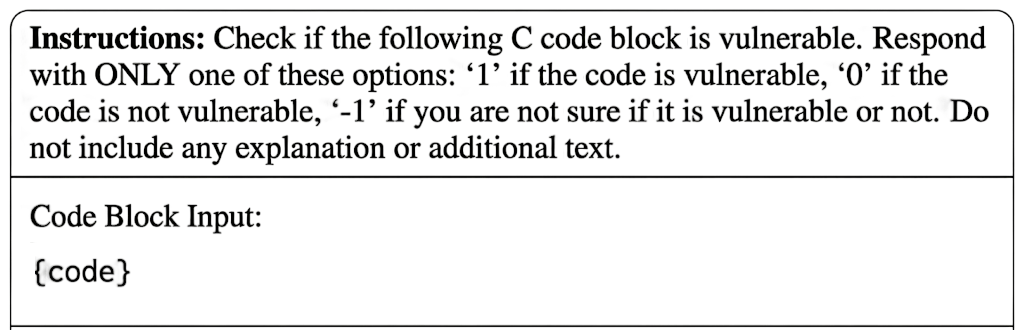
\includegraphics[width=1\columnwidth]{figures/promptSVD3.png}}
%DIFDELCMD < 	%%%
\DIFdelendFL \DIFaddbeginFL \centering
\DIFaddFL{\fbox{\begin{minipage}{0.94\columnwidth}
\ttfamily\footnotesize
Check if the following C code block is vulnerable.\\
Respond with ONLY one of these options:\\
- '1' if the code is vulnerable\\
- '0' if the code is not vulnerable\\
- 'not sure' if you are not sure if it is vulnerable or not\\[2pt]
Do not include any explanation or additional text.\\[2pt]
Code block:\\
\{code\}\\[2pt]
Response:
\end{minipage}}
	}\DIFaddendFL \caption{\DIFdelbeginFL \DIFdelFL{Vulnerability detection and }\DIFdelendFL \DIFaddbeginFL \DIFaddFL{Verbatim vulnerability-detection template used in the production pipeline; }\DIFaddendFL patch verification \DIFdelbeginFL \DIFdelFL{prompt}\DIFdelendFL \DIFaddbeginFL \DIFaddFL{substitutes the patched code block}\DIFaddendFL .}
	\label{figure:prompt_svd3}
\end{figure}
\begin{figure}[!t]
\centerline{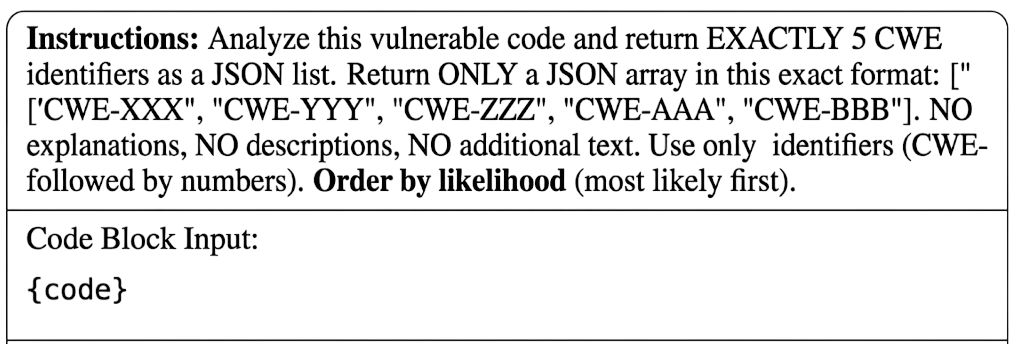
\includegraphics[width=1.0\columnwidth]{figures/promptSVD2.png}}
	\caption{\gls{CWE} ranking prompt.}
	\label{figure:prompt_svd2}
\end{figure}
\DIFaddbegin 

\DIFaddend Our prompt templates for both \gls{SVD} and CWE-label classification are designed with four key principles in mind: clear task specification, structured output formats, minimal introduction of bias, and scalability across vulnerability types. We focus on benchmarking the inherent \gls{LLM} capabilities rather than optimizing prompting strategies, and on evaluating baseline performance to inform future research directions. \DIFdelbegin \DIFdel{Each }\DIFdelend \DIFaddbegin \DIFadd{As shown in Figure~\ref{figure:prompt_svd3}, each }\DIFaddend prompt clearly states the expected task and output format, \DIFaddbegin \DIFadd{including explicit three-way response instructions (}\texttt{\DIFadd{1}}\DIFadd{, }\texttt{\DIFadd{0}}\DIFadd{, or }\texttt{\DIFadd{not sure}}\DIFadd{; the uncertainty response is stored as }\texttt{\DIFadd{-1}} \DIFadd{for evaluation), }\DIFaddend uses standardized templates for fair comparison across models, maintains essential code context while avoiding information leakage, and reflects real-world security analysis scenarios.

Representative prompt formats are shown in Figures~\ref{figure:prompt_svd3} (\gls{SVD}) and~\ref{figure:prompt_svd2} (CWE-label classification).

%\begin{table}[h!]
%\centering
%\captionsetup{skip=2pt,font=small}
%\caption{Prompt Templates for SVD and \gls{SPV} Tasks}
%\label{table:prompt_templates}
%\setlength{\tabcolsep}{1.5pt}
%\renewcommand{\arraystretch}{0.9}
%{\scriptsize
%\begin{tabularx}{\columnwidth}{@{\extracolsep{\fill}}%
%l l
%>{\centering\arraybackslash}p{0.053\columnwidth}%
%>{\centering\arraybackslash}p{0.053\columnwidth}%
%>{\centering\arraybackslash}p{0.060\columnwidth}%
%>{\centering\arraybackslash}p{0.060\columnwidth}%
%X@{}}
%\toprule
%\multicolumn{1}{c}{\textbf{ID}} &
%\multicolumn{1}{c}{\textbf{Task}} &
%\multicolumn{4}{c}{\textbf{Inputs}} &
%\multicolumn{1}{c}{\textbf{Description}} \\
%\cmidrule(lr){3-6}
%& & \multicolumn{1}{c}{\textbf{V}} &
%\multicolumn{1}{c}{\textbf{P}} &
%\multicolumn{1}{c}{\textbf{CVE}} &
%\multicolumn{1}{c}{\textbf{CWE}} & \\
%\midrule
%SVD2 & \gls{CWE} Ranking  & Y  & -- & -- & -- & Rank top-5 CWEs for given code. \\
%SVD3 & Detection    & Y  & -- & -- & -- & Detect whether code is vulnerable (non-targeted). \\
%SVD4 & Verification & -- & Y  & -- & -- & Verify patched code is safe (non-targeted). \\
%SVD5 & Detection    & Y  & -- & Y  & Y  & Detect vulnerability for a specific CVE/\gls{CWE} (targeted). \\
%SVD6 & Verification & -- & Y  & Y  & Y  & Verify patch for a specific CVE/\gls{CWE} (targeted). \\
%\bottomrule
%\end{tabularx}
%}
%\vspace{2pt}
%\raggedright\scriptsize
%V: vulnerable code (pre-fix); P: patched code (post-fix). All tasks use zero-shot prompts.
%\end{table}



\section{Benchmarking Results}
\label{section:results}

In this study, we leverage seven pre-trained \glspl{LLM} to assess their capabilities in \gls{SVD} and CWE-label classification tasks. Our selection comprises three code-specialized models (CodeLlama~\cite{roziere2023code}, StarCoder2 \cite{lozhkov2024starcoder}, and \DIFdelbegin \DIFdel{Qwen2.5-Coder}\DIFdelend \DIFaddbegin \DIFadd{Qwen3-Coder}\DIFaddend ~\cite{yang2025qwen3}) explicitly trained on programming repositories, and four general-purpose models (Llama3.1~\cite{dubey2024llama}, Mistral~\cite{jiang2023mistral7b}, and DeepSeek-R1~\cite{guo2025deepseek}, GPT-4.1-mini~\cite{openai2025gpt4_1mini}) designed for broader language understanding tasks. This balanced selection enables us to investigate whether domain-specific training provides advantages over general language comprehension for security-critical tasks. We selected these models based on five key criteria: (1) their state-of-the-art performance on code understanding and generation benchmarks, (2) architectural diversity spanning both standard fully-dense models (e.g., CodeLlama) and \gls{MoE} models (e.g., DeepSeek-R1) to ensure comprehensive evaluation, (3) varying parameter sizes (7B-30B and unknown for GPT-4.1-mini) and context window capacities (16K-1M tokens) to investigate how model scale and memory affect \gls{SVD} capabilities, (4) balanced representation of code-specialized versus general-purpose training to assess domain expertise effects, and (5) inclusion of both smaller open-source and larger proprietary models, allowing for a fair comparison across accessibility and capability dimensions. The specifications of the models we used are detailed in Table~\ref{table:llm-specs}.

\begin{table}[!t]
\centering
\caption{LLM specs with context window sizes (tokens).}
\label{table:llm-specs}
\footnotesize
\setlength{\tabcolsep}{6pt}
\renewcommand{\arraystretch}{1.1}
\begin{tabular}{@{}l l r r@{}}
\toprule
\textbf{Model} & \textbf{Type} & \textbf{\# Params} & \textbf{Context Window} \\
\midrule
CodeLlama & Code-spec. & 7B & 16K \\
StarCoder2 & Code-spec. & 7B & 16K \\
\DIFdelbeginFL \DIFdelFL{Qwen2.5-Coder }\DIFdelendFL \DIFaddbeginFL \DIFaddFL{Qwen3-Coder }\DIFaddendFL & Code-spec. & 30B & 262K \\
Llama3.1 & General & 8B & 131K \\
Mistral (v0.3) & General & 7B & 32K \\
DeepSeek-R1 & General & 7B & 131K \\
GPT-4.1-mini & General & --- & 1M \\
\bottomrule
\end{tabular}
\end{table}

\subsection{RQ1: Overall \gls{SVD} performance}
\DIFaddbegin \label{section:rq1}
\DIFaddend 

For this research question, we \DIFdelbegin \DIFdel{divide our analysis into two parts. First, we analyze model performance in the }\DIFdelend \DIFaddbegin \DIFadd{first separate valid binary verdicts from genuine abstentions and invalid outputs. We then analyze classification performance in two settings: }\DIFaddend non-targeted\DIFdelbegin \DIFdel{setting, where models are asked to classify code as vulnerable}\DIFdelend \DIFaddbegin \DIFadd{, where no specific CWE is provided, and targeted, where the prompt includes the CWE label. Because the validated response rates supplied for this audit are pooled over both settings and both datasets, Table~\ref{tab:abst-model-non-targeted} reports the overall temperature-0 response distribution rather than unsupported setting-specific estimates. Each available model contributes 1,668 responses (417 vulnerable}\DIFaddend /\DIFdelbegin \DIFdel{non-vulnerable with no information about the specific CWE . Then, we repeat the same analysis but for the targetedsetting, where models are given the \mbox{%DIFAUXCMD
\gls{CWE} }\hskip0pt%DIFAUXCMD
label in the prompt . Within each of these parts, we start by looking at how often each model actually provided an answer (regardless of its correctness) and how often it refused to answer (-1), and then look into the values for the metrics (accuracy, recall, and precision).
}\DIFdelend \DIFaddbegin \DIFadd{patched pairs evaluated in both settings).
}\DIFaddend 

\DIFdelbegin \subsubsection{\DIFdel{Non-targeted Classification}}
%DIFAUXCMD
\addtocounter{subsubsection}{-1}%DIFAUXCMD
%DIFDELCMD < 

%DIFDELCMD < \begin{table}[!t]
%DIFDELCMD < %%%
\DIFdelendFL \DIFaddbeginFL \begin{table}[h]
\DIFaddendFL \centering\DIFdelbeginFL %DIFDELCMD < \caption{%
{%DIFAUXCMD
\DIFdelFL{Abstention rates (\%) for non-targeted and targeted \mbox{%DIFAUXCMD
\gls{SVD}}\hskip0pt%DIFAUXCMD
.}}
%DIFAUXCMD
%DIFDELCMD < \label{tab:res-dist-abstention}
%DIFDELCMD < \small
%DIFDELCMD < \setlength{\tabcolsep}{10pt}
%DIFDELCMD < \renewcommand{\arraystretch}{1.05}
%DIFDELCMD < \resizebox{\columnwidth}{!}{%
%DIFDELCMD < \begin{tabular}{lcccc}
%DIFDELCMD < \toprule
%DIFDELCMD < & \multicolumn{2}{c}{\textbf{Non-Targeted}} & \multicolumn{2}{c}{\textbf{Targeted}} \\
%DIFDELCMD < \cmidrule(lr){2-3} \cmidrule(lr){4-5}
%DIFDELCMD < \textbf{Model} & PBD (\%) & LFD (\%) & PBD (\%) & LFD (\%) \\
%DIFDELCMD < \midrule
%DIFDELCMD < CodeLlama    & 0.5 & 0.0 & 0.3 & 0.0 \\
%DIFDELCMD < DeepSeek     & 30.4 & 24.3 & 6.1 & 7.3 \\
%DIFDELCMD < GPT-4.1-mini & 2.2 & 3.9 & 1.1 & 1.5 \\
%DIFDELCMD < Llama3.1     & 52.6 & 59.7 & 51.9 & 55.8 \\
%DIFDELCMD < Mistral      & 0.0 & 0.0 & 0.0 & 0.0 \\
%DIFDELCMD < Qwen2.5-Coder  & 34.7 & 37.9 & 46.7 & 37.9 \\
%DIFDELCMD < StarCoder2   & 16.9 & 22.3 & 11.3 & 21.4 \\
%DIFDELCMD < \bottomrule
%DIFDELCMD < \end{tabular}
%DIFDELCMD < }
%DIFDELCMD < \end{table}
%DIFDELCMD < 

%DIFDELCMD < %%%
\textbf{\DIFdel{Models exhibit substantial differences in abstention behavior.}} %DIFAUXCMD
\DIFdel{Table~\ref{tab:res-dist-abstention} shows abstention rates across both non-targeted and targeted settings. CodeLlama, }\DIFdelend %DIF > \color{red}
\DIFaddbegin \caption{\DIFadd{Response validity at temperature 0, pooled over non-targeted/targeted settings and PBD/LFD. }\emph{\DIFadd{Valid}}\DIFadd{: a resolvable 0/1 verdict; }\emph{\DIFadd{Genuine abstention}}\DIFadd{: a clear uncertainty verdict; }\emph{\DIFadd{Invalid}}\DIFadd{: non-compliant or indeterminate output. GPT-4.1-mini was not run at this temperature.}}
\label{tab:abst-model-non-targeted}
\begin{tabular}{lrrr}
\hline
\textbf{\DIFadd{Model}} & \textbf{\DIFadd{Valid (\%)}} & \textbf{\DIFadd{Genuine abst.\ (\%)}} & \textbf{\DIFadd{Invalid (\%)}} \\
\hline
\DIFadd{CodeLlama       }& \DIFadd{98.20 }& \DIFadd{0.00 }& \DIFadd{1.80 }\\
\DIFadd{DeepSeek-R1     }& \DIFadd{100.00 }& \DIFadd{0.00 }& \DIFadd{0.00 }\\
\DIFaddend GPT-4.1-mini    \DIFdelbegin \DIFdel{, and Mistral         consistently provide predictions, with abstention rates below 4\%across all conditions. Mistral never abstains, while CodeLlama abstains in only 0.5\% of non-targeted PBD cases. In contrast, }\DIFdelend \DIFaddbegin & \DIFadd{-- }& \DIFadd{-- }& \DIFadd{-- }\\
\DIFaddend Llama3.1        \DIFdelbegin \DIFdel{abstains in over half of all queries (52.6\% –59.7\%), refusing to commit to classifications even when CVE/CWE context is provided. DeepSeek and Qwen2.5-Coder show intermediate but asymmetric behavior: DeepSeek's abstention drops sharply from 30.4\% (non-targeted) to 6.1\% (targeted) in PBD, while Qwen2.5-Coder's abstention increases from 34.7\% to 46.7\%. Providing explicit vulnerability context does not consistently reduce abstention: }\DIFdelend \DIFaddbegin & \DIFadd{100.00 }& \DIFadd{0.00 }& \DIFadd{0.00 }\\
\DIFadd{Mistral         }& \DIFadd{98.62 }& \DIFadd{0.00 }& \DIFadd{1.38 }\\
\DIFadd{Qwen3-Coder-30B }& \DIFadd{99.46 }& \DIFadd{0.06 }& \DIFadd{0.48 }\\
\DIFadd{StarCoder2      }& \DIFadd{73.92 }& \DIFadd{0.00 }& \DIFadd{26.08 }\\
\hline
\end{tabular}
\end{table}

\textbf{\DIFadd{Genuine abstention is rare, while most non-answers are formatting failures.}}
\DIFadd{At temperature 0, Qwen3-Coder is the only model with observed genuine abstentions (0.06\%). The other open-source models have no genuine abstentions. Invalid output is below 2\% for CodeLlama, Mistral, and Qwen3-Coder, and absent for DeepSeek-R1 and }\DIFaddend Llama3.1\DIFdelbegin \DIFdel{and Qwen2.5-Coder remain highly conservative across task types, revealing fundamental differences in model confidence calibration rather than task-specific uncertainty.
}\DIFdelend \DIFaddbegin \DIFadd{. StarCoder2 is the clear exception: 26.08\% of its outputs are invalid, primarily because the base completion model continues code or otherwise fails to emit one of the requested verdicts. The broader decoding sweep in Table~\ref{tab:abst-temp} confirms that genuine abstention and invalid output are distinct behaviors: GPT-4.1-mini averages 2.40\% genuine abstention across the two temperature-0.1 runs, while StarCoder2's invalid rate reaches 26.08\% at temperature 0.
}\DIFaddend 

\DIFaddbegin \subsubsection{\DIFadd{Non-targeted Classification}}
\label{section:rq1-nontargeted}

\DIFaddend \textbf{\glspl{LLM} performed no better than random classifiers.} \DIFdelbegin \DIFdel{In the non-targeted setting, }\DIFdelend Table~\ref{tab:metrics-svd} \DIFdelbegin \DIFdel{(Non-Targeted columns) presents the actual performance metrics , considering only }\DIFdelend \DIFaddbegin \DIFadd{presents }\DIFaddend the \DIFaddbegin \DIFadd{performance metrics for the }\DIFaddend cases where the models \DIFdelbegin \DIFdel{did provide }\DIFdelend \DIFaddbegin \DIFadd{provided }\DIFaddend a classification. \DIFdelbegin \DIFdel{We can see that all }\DIFdelend \DIFaddbegin \DIFadd{All }\DIFaddend models exhibit accuracies close to 50\%, irrespective of architecture, size, or context window size. This \DIFdelbegin \DIFdel{performance can be seen in both the }\DIFdelend \DIFaddbegin \DIFadd{behaviour is observed on both }\DIFaddend \gls{PBD} and \gls{LFD}\DIFdelbegin \DIFdel{, indicating that potential training data leakage had no effect on performance and that none of the models have truly learned meaningful patterns to distinguish between vulnerable and non-vulnerable code in this setting}\DIFdelend \DIFaddbegin \DIFadd{; the historical split does not show a clear aggregate advantage over the post-cutoff split. Because the splits differ in composition and size, this comparison constrains but does not isolate the causal effect of training-data exposure}\DIFaddend .

Consider CVE-2024-26599 (CWE-119, PBD), a clear out-of-bounds array access in a PWM driver function (Figure~\ref{figure:cve_2024_26599}). The vulnerable code \DIFdelbegin \DIFdel{checks }\DIFdelend \DIFaddbegin \DIFadd{validates that }\DIFaddend \texttt{args->args\_count\DIFdelbegin \DIFdel{!= 1 \&\& args->args\_count != 2}\DIFdelend } \DIFdelbegin \DIFdel{to validate input, then }\DIFdelend \DIFaddbegin \DIFadd{is either 1 or 2, but subsequently }\DIFaddend accesses \texttt{args->args[2]} when \texttt{args\_count == 2}. \DIFdelbegin \DIFdel{This is an obvious bug: if an array has count=2}\DIFdelend \DIFaddbegin \DIFadd{Since arrays are zero-indexed}\DIFaddend , valid indices are \DIFaddbegin \DIFadd{only }\DIFaddend 0 and 1\DIFdelbegin \DIFdel{(zero-indexed), so index 2 is out of bounds. The fix simply changes }\DIFdelend \DIFaddbegin \DIFadd{, making this an obvious out-of-bounds access. The patch simply replaces }\DIFaddend \texttt{args[2]} \DIFdelbegin \DIFdel{to }\DIFdelend \DIFaddbegin \DIFadd{with }\DIFaddend \texttt{args[1]}. A human reviewer can immediately identify this as vulnerable because it violates \DIFdelbegin \DIFdel{basic array indexing rules. Yet all four major models failed: Codellama and Mistral incorrectly classified both }\DIFdelend \DIFaddbegin \DIFadd{a basic array bounds constraint. Yet the models still struggled to distinguish the vulnerable and patched versions reliably. In the first run, GPT-4.1-mini correctly classified both the }\DIFaddend vulnerable and patched \DIFdelbegin \DIFdel{versions }\DIFdelend \DIFaddbegin \DIFadd{samples. CodeLlama, Mistral, and DeepSeek classified both }\DIFaddend as vulnerable, \DIFdelbegin \DIFdel{Deepseek }\DIFdelend \DIFaddbegin \DIFadd{while Llama3.1 }\DIFaddend classified both as safe\DIFdelbegin \DIFdel{, and Llama abstained on both. This demonstrates that the dataset contains clear, detectable vulnerabilities with sufficient context, but models simply lack the fundamental security reasoning to identify even straightforward bounds violations}\DIFdelend . \DIFaddbegin \DIFadd{StarCoder2 produced an invalid response for the vulnerable version and classified the patched version as safe. This example is consistent with the aggregate class biases in Table~\ref{tab:metrics-svd}: even when the local defect is explicit, several models preserve the same verdict across the vulnerable--patched pair rather than responding to the changed array index.
}\DIFaddend 

\DIFaddbegin \DIFadd{These results stand in sharp contrast to supervised detection tools evaluated under different assumptions: SecureFalcon~\mbox{%DIFAUXCMD
\cite{ferrag2025securefalcon} }\hskip0pt%DIFAUXCMD
reports 94\% binary accuracy on C/C++ code after training on FormAI/FalconVulnDB, and Alam et al.\ report 99\% Solidity vulnerability-detection accuracy after fine-tuning GPT-3.5 Turbo and GPT-4o Mini~\mbox{%DIFAUXCMD
\cite{alam2024detection}}\hskip0pt%DIFAUXCMD
. These figures are not directly comparable because the studies use task-specific training datasets and different software domains, whereas our evaluation measures zero-shot, off-the-shelf performance and includes a post-cutoff split.
}

\DIFaddend \begin{figure}[!t]

\begin{lstlisting}[language=Diff, basicstyle=\scriptsize\ttfamily, xleftmargin=0pt, frame=single]
// File: drivers/pwm/core.c
of_pwm_single_xlate(struct pwm_chip *chip,
                    const struct of_phandle_args *args) {
    struct pwm_device *pwm;

    if (chip->of_pwm_n_cells < 1)
        return ERR_PTR(-EINVAL);

    // Validates that args_count is either 1 or 2
    if (args->args_count != 1 && args->args_count != 2)
        return ERR_PTR(-EINVAL);

    pwm = pwm_request_from_chip(chip, 0, NULL);
    if (IS_ERR(pwm))
        return pwm;

    pwm->args.period = args->args[0];
    pwm->args.polarity = PWM_POLARITY_NORMAL;

    // BUG: Accessing index 2 when count==2 (valid: 0,1)
-   if (args->args_count == 2 && args->args[2] & PWM_POLARITY_INVERTED)
+   if (args->args_count == 2 && args->args[1] & PWM_POLARITY_INVERTED)
        pwm->args.polarity = PWM_POLARITY_INVERSED;

    return pwm;
}
\end{lstlisting}

\caption{CVE-2024-26599: out-of-bounds access; patch shown.}
\label{figure:cve_2024_26599}
\end{figure}

\textbf{Models \DIFdelbegin \DIFdel{tend to have an extreme bias towards one of the classes}\DIFdelend \DIFaddbegin \DIFadd{exhibit strong and consistent class biases rather than meaningful vulnerability detection behaviour}\DIFaddend .} Examining \DIFdelbegin \DIFdel{metrics such as }\DIFdelend Recall, Precision, and \gls{PPR} reveals \DIFdelbegin \DIFdel{consistent }\DIFdelend \DIFaddbegin \DIFadd{clear }\DIFaddend patterns across both \DIFdelbegin \DIFdel{the \mbox{%DIFAUXCMD
\gls{PBD} }\hskip0pt%DIFAUXCMD
and \mbox{%DIFAUXCMD
\gls{LFD}}\hskip0pt%DIFAUXCMD
. CodeLlama and Mistralstand out in both datasets with }\DIFdelend \DIFaddbegin \DIFadd{datasets. In the non-targeted setting, CodeLlama, DeepSeek, Mistral, and Qwen3-Coder all achieve }\DIFaddend very high recall values (\DIFdelbegin \DIFdel{around 75–88\%for PBD and 70–81\% for LFD) , indicating that they correctly flag most vulnerable samples }\DIFdelend \DIFaddbegin \DIFadd{roughly 70--85\%) together with high \mbox{%DIFAUXCMD
\gls{PPR} }\hskip0pt%DIFAUXCMD
values, indicating a strong tendency to classify most samples as vulnerable}\DIFaddend . However, their \DIFdelbegin \DIFdel{corresponding precision and \mbox{%DIFAUXCMD
\gls{PPR} }\hskip0pt%DIFAUXCMD
values (around }\DIFdelend \DIFaddbegin \DIFadd{precision remains close to }\DIFaddend 50\%\DIFdelbegin \DIFdel{precision and 0.8 \mbox{%DIFAUXCMD
\gls{PPR}}\hskip0pt%DIFAUXCMD
) indicate }\DIFdelend \DIFaddbegin \DIFadd{, showing }\DIFaddend that these high recall scores are \DIFdelbegin \DIFdel{driven by a strong bias toward positive predictions: the models tend to classify most samples as vulnerable, regardless of the true label. }%DIFDELCMD < 

%DIFDELCMD < %%%
\DIFdelend \DIFaddbegin \DIFadd{largely driven by overpredicting the positive class rather than correctly identifying vulnerabilities. }\DIFaddend In contrast, \DIFdelbegin \DIFdel{models such as }\DIFdelend GPT-4.1-mini \DIFdelbegin \DIFdel{, }\DIFdelend \DIFaddbegin \DIFadd{and }\DIFaddend Llama3.1 \DIFdelbegin \DIFdel{, Qwen2.5-Coder, and DeepSeek }\DIFdelend exhibit the opposite behaviour\DIFdelbegin \DIFdel{across both datasets. Their }\DIFdelend \DIFaddbegin \DIFadd{, with }\DIFaddend low recall and \DIFdelbegin \DIFdel{\mbox{%DIFAUXCMD
\gls{PPR} }\hskip0pt%DIFAUXCMD
values indicate }\DIFdelend \DIFaddbegin \DIFadd{low \mbox{%DIFAUXCMD
\gls{PPR} }\hskip0pt%DIFAUXCMD
values across both datasets, indicating }\DIFaddend a strong bias toward \DIFdelbegin \DIFdel{the negative class (}\DIFdelend \DIFaddbegin \DIFadd{predicting samples as }\DIFaddend non-vulnerable\DIFdelbegin \DIFdel{code), with most predictions defaulting to }%DIFDELCMD < \enquote{not vulnerable}%%%
\DIFdel{. Yet despite }\DIFdelend \DIFaddbegin \DIFadd{. Despite }\DIFaddend this conservative tendency, \DIFdelbegin \DIFdel{their precision remains low, so even when these models predict a vulnerability, they are often incorrect. }%DIFDELCMD < 

%DIFDELCMD < %%%
\DIFdel{Overall, these patterns are remarkably consistent across the PBD and LFD, reinforcing the conclusion that the observed biases are intrinsic to the models rather than a result of training data leakage or dataset-specific artifacts}\DIFdelend \DIFaddbegin \DIFadd{precision also remains close to random, meaning that even its positive predictions are unreliable. StarCoder2 appears comparatively more balanced, with recall and \mbox{%DIFAUXCMD
\gls{PPR} }\hskip0pt%DIFAUXCMD
values closer to 50\%, but its overall accuracy still remains at chance level}\DIFaddend .


\begin{table*}[!t]
    %DIF > \color{red}
    \centering
    \caption{Performance metrics for \gls{SVD} in non-targeted and targeted settings.}
    \label{tab:metrics-svd}
    \scriptsize
    \renewcommand{\arraystretch}{1.0}
    \DIFdelbeginFL %DIFDELCMD < \setlength{\tabcolsep}{1.8pt}
%DIFDELCMD <     %%%
\DIFdelendFL %DIF > \setlength{\tabcolsep}{1.8pt}
    \begin{tabular}{l rr rr rr rr rr rr rr rr}
    \toprule
    \multirow{3}{*}{Model}
      & \multicolumn{8}{c}{\textbf{Non-Targeted}}
      & \multicolumn{8}{c}{\textbf{Targeted}} \\
    \cmidrule(lr){2-9} \cmidrule(lr){10-17}
      & \multicolumn{4}{c}{PBD (\%)} & \multicolumn{4}{c}{LFD (\%)}
      & \multicolumn{4}{c}{PBD (\%)} & \multicolumn{4}{c}{LFD (\%)} \\
    \cmidrule(lr){2-5} \cmidrule(lr){6-9} \cmidrule(lr){10-13} \cmidrule(lr){14-17}
      & Acc. & Rec. & Prec. & PPR 
      & Acc. & Rec. & Prec. & PPR 
      & Acc. & Rec. & Prec. & PPR 
      & Acc. & Rec. & Prec. & PPR \\
    \midrule
    CodeLlama & \DIFdelbeginFL \DIFdelFL{49.0 }\DIFdelendFL \DIFaddbeginFL \DIFaddFL{49.9 }\DIFaddendFL & \DIFdelbeginFL \DIFdelFL{75.7 }\DIFdelendFL \DIFaddbeginFL \DIFaddFL{73.3 }\DIFaddendFL & \DIFdelbeginFL \DIFdelFL{49.4 }\DIFdelendFL \DIFaddbeginFL \DIFaddFL{49.9 }\DIFaddendFL & \DIFdelbeginFL \DIFdelFL{76.8 }\DIFdelendFL \DIFaddbeginFL \DIFaddFL{73.5 }\DIFaddendFL & \DIFdelbeginFL \DIFdelFL{51.0 }\DIFdelendFL \DIFaddbeginFL \DIFaddFL{50.5 }\DIFaddendFL & \DIFdelbeginFL \DIFdelFL{70.9 }\DIFdelendFL \DIFaddbeginFL \DIFaddFL{69.9	}\DIFaddendFL & \DIFdelbeginFL \DIFdelFL{50.7 }\DIFdelendFL \DIFaddbeginFL \DIFaddFL{50.3 }\DIFaddendFL & \DIFdelbeginFL \DIFdelFL{69.9 }\DIFdelendFL \DIFaddbeginFL \DIFaddFL{69.4 }\DIFaddendFL & \DIFdelbeginFL \DIFdelFL{52.2 }\DIFdelendFL \DIFaddbeginFL \DIFaddFL{51.7 }\DIFaddendFL & \DIFdelbeginFL \DIFdelFL{92.0 }\DIFdelendFL \DIFaddbeginFL \DIFaddFL{88.2 }\DIFaddendFL & \DIFdelbeginFL \DIFdelFL{51.2 }\DIFdelendFL \DIFaddbeginFL \DIFaddFL{51.0 }\DIFaddendFL & \DIFdelbeginFL \DIFdelFL{89.9 }\DIFdelendFL \DIFaddbeginFL \DIFaddFL{86.6 }\DIFaddendFL & \DIFdelbeginFL \DIFdelFL{56.8 }\DIFdelendFL \DIFaddbeginFL \DIFaddFL{52.9 }\DIFaddendFL & \DIFdelbeginFL \DIFdelFL{92.2 }\DIFdelendFL \DIFaddbeginFL \DIFaddFL{90.0 }\DIFaddendFL & \DIFdelbeginFL \DIFdelFL{54.0 }\DIFdelendFL \DIFaddbeginFL \DIFaddFL{51.7 }\DIFaddendFL & \DIFdelbeginFL \DIFdelFL{85.4 }\DIFdelendFL \DIFaddbeginFL \DIFaddFL{87.1 }\DIFaddendFL \\
    DeepSeek & \DIFdelbeginFL \DIFdelFL{51.3 }\DIFdelendFL \DIFaddbeginFL \DIFaddFL{49.6 }\DIFaddendFL & \DIFdelbeginFL \DIFdelFL{16.0 }\DIFdelendFL \DIFaddbeginFL \DIFaddFL{81.3 }\DIFaddendFL & \DIFdelbeginFL \DIFdelFL{49.2 }\DIFdelendFL \DIFaddbeginFL \DIFaddFL{50.1 }\DIFaddendFL & \DIFdelbeginFL \DIFdelFL{15.7 }\DIFdelendFL \DIFaddbeginFL \DIFaddFL{80.1 }\DIFaddendFL & \DIFdelbeginFL \DIFdelFL{46.9 }\DIFdelendFL \DIFaddbeginFL \DIFaddFL{50.0 }\DIFaddendFL & \DIFdelbeginFL \DIFdelFL{11.5 }\DIFdelendFL \DIFaddbeginFL \DIFaddFL{77.7 }\DIFaddendFL & \DIFdelbeginFL \DIFdelFL{52.9 }\DIFdelendFL \DIFaddbeginFL \DIFaddFL{50.0 }\DIFaddendFL & \DIFdelbeginFL \DIFdelFL{11.7 }\DIFdelendFL \DIFaddbeginFL \DIFaddFL{77.7 }\DIFaddendFL & \DIFdelbeginFL \DIFdelFL{46.5 }\DIFdelendFL \DIFaddbeginFL \DIFaddFL{49.6 }\DIFaddendFL & \DIFdelbeginFL \DIFdelFL{44.5 }\DIFdelendFL \DIFaddbeginFL \DIFaddFL{87.3 }\DIFaddendFL & \DIFdelbeginFL \DIFdelFL{44.7 }\DIFdelendFL \DIFaddbeginFL \DIFaddFL{50.2 }\DIFaddendFL & \DIFdelbeginFL \DIFdelFL{48.2 }\DIFdelendFL \DIFaddbeginFL \DIFaddFL{86.1 }\DIFaddendFL & \DIFdelbeginFL \DIFdelFL{50.3 }\DIFdelendFL \DIFaddbeginFL \DIFaddFL{51.9 }\DIFaddendFL & \DIFdelbeginFL \DIFdelFL{42.3 }\DIFdelendFL \DIFaddbeginFL \DIFaddFL{86.4 }\DIFaddendFL & \DIFdelbeginFL \DIFdelFL{55.0 }\DIFdelendFL \DIFaddbeginFL \DIFaddFL{51.3 }\DIFaddendFL & \DIFdelbeginFL \DIFdelFL{41.4 }\DIFdelendFL \DIFaddbeginFL \DIFaddFL{84.5 }\DIFaddendFL \\
    GPT-4.1-mini & \DIFdelbeginFL \DIFdelFL{50.7 }\DIFdelendFL \DIFaddbeginFL \DIFaddFL{50.8 }\DIFaddendFL & \DIFdelbeginFL \DIFdelFL{5.8 }\DIFdelendFL \DIFaddbeginFL \DIFaddFL{5.2 }\DIFaddendFL & \DIFdelbeginFL \DIFdelFL{60.0 }\DIFdelendFL \DIFaddbeginFL \DIFaddFL{59.9 }\DIFaddendFL & \DIFdelbeginFL \DIFdelFL{4.9 }\DIFdelendFL \DIFaddbeginFL \DIFaddFL{4.4 }\DIFaddendFL & \DIFdelbeginFL \DIFdelFL{51.8 }\DIFdelendFL \DIFaddbeginFL \DIFaddFL{51.5 }\DIFaddendFL & \DIFdelbeginFL \DIFdelFL{4.2 }\DIFdelendFL \DIFaddbeginFL \DIFaddFL{5.5 }\DIFaddendFL & \DIFdelbeginFL \DIFdelFL{66.7 }\DIFdelendFL \DIFaddbeginFL \DIFaddFL{70.0 }\DIFaddendFL & \DIFdelbeginFL \DIFdelFL{3.1 }\DIFdelendFL \DIFaddbeginFL \DIFaddFL{4.0 }\DIFaddendFL & \DIFdelbeginFL \DIFdelFL{49.5 }\DIFdelendFL \DIFaddbeginFL \DIFaddFL{49.6 }\DIFaddendFL & \DIFdelbeginFL \DIFdelFL{7.8 }\DIFdelendFL \DIFaddbeginFL \DIFaddFL{7.4 }\DIFaddendFL & \DIFdelbeginFL \DIFdelFL{49.0 }\DIFdelendFL \DIFaddbeginFL \DIFaddFL{47.3 }\DIFaddendFL & \DIFdelbeginFL \DIFdelFL{8.0 }\DIFdelendFL \DIFaddbeginFL \DIFaddFL{7.9 }\DIFaddendFL & \DIFdelbeginFL \DIFdelFL{53.3 }\DIFdelendFL \DIFaddbeginFL \DIFaddFL{52.6 }\DIFaddendFL & \DIFdelbeginFL \DIFdelFL{7.3 }\DIFdelendFL \DIFaddbeginFL \DIFaddFL{8.4 }\DIFaddendFL & \DIFdelbeginFL \DIFdelFL{77.8 }\DIFdelendFL \DIFaddbeginFL \DIFaddFL{72.6 }\DIFaddendFL & \DIFdelbeginFL \DIFdelFL{4.6 }\DIFdelendFL \DIFaddbeginFL \DIFaddFL{5.8 }\DIFaddendFL \\
    Llama3.1 & \DIFdelbeginFL \DIFdelFL{45.0 }\DIFdelendFL \DIFaddbeginFL \DIFaddFL{50.1 }\DIFaddendFL & \DIFdelbeginFL \DIFdelFL{3.1 }\DIFdelendFL \DIFaddbeginFL \DIFaddFL{31.6 }\DIFaddendFL & \DIFdelbeginFL \DIFdelFL{33.3 }\DIFdelendFL \DIFaddbeginFL \DIFaddFL{50.1 }\DIFaddendFL & \DIFdelbeginFL \DIFdelFL{5.0 }\DIFdelendFL \DIFaddbeginFL \DIFaddFL{31.5 }\DIFaddendFL & \DIFdelbeginFL \DIFdelFL{40.9 }\DIFdelendFL \DIFaddbeginFL \DIFaddFL{51.0 }\DIFaddendFL & \DIFdelbeginFL \DIFdelFL{0.0 }\DIFdelendFL \DIFaddbeginFL \DIFaddFL{29.4 }\DIFaddendFL & \DIFdelbeginFL \DIFdelFL{0.0 }\DIFdelendFL \DIFaddbeginFL \DIFaddFL{51.6 }\DIFaddendFL & \DIFdelbeginFL \DIFdelFL{0.0 }\DIFdelendFL \DIFaddbeginFL \DIFaddFL{28.5 }\DIFaddendFL & \DIFdelbeginFL \DIFdelFL{46.7 }\DIFdelendFL \DIFaddbeginFL \DIFaddFL{49.4 }\DIFaddendFL & \DIFdelbeginFL \DIFdelFL{0.0 }\DIFdelendFL \DIFaddbeginFL \DIFaddFL{27.3 }\DIFaddendFL & \DIFdelbeginFL \DIFdelFL{0.0 }\DIFdelendFL \DIFaddbeginFL \DIFaddFL{48.9 }\DIFaddendFL & \DIFdelbeginFL \DIFdelFL{0.0 }\DIFdelendFL \DIFaddbeginFL \DIFaddFL{27.9 }\DIFaddendFL & \DIFdelbeginFL \DIFdelFL{40.9 }\DIFdelendFL \DIFaddbeginFL \DIFaddFL{47.7 }\DIFaddendFL & \DIFdelbeginFL \DIFdelFL{0.0 }\DIFdelendFL \DIFaddbeginFL \DIFaddFL{15.5 }\DIFaddendFL & \DIFdelbeginFL \DIFdelFL{0.0 }\DIFdelendFL \DIFaddbeginFL \DIFaddFL{43.6 }\DIFaddendFL & \DIFdelbeginFL \DIFdelFL{0.0 }\DIFdelendFL \DIFaddbeginFL \DIFaddFL{17.8 }\DIFaddendFL \\
    Mistral & 49.4 & \DIFdelbeginFL \DIFdelFL{88.2 }\DIFdelendFL \DIFaddbeginFL \DIFaddFL{85.2 }\DIFaddendFL & \DIFdelbeginFL \DIFdelFL{49.6 }\DIFdelendFL \DIFaddbeginFL \DIFaddFL{49.7 }\DIFaddendFL & \DIFdelbeginFL \DIFdelFL{88.9 }\DIFdelendFL \DIFaddbeginFL \DIFaddFL{85.8 }\DIFaddendFL & \DIFdelbeginFL \DIFdelFL{51.0 }\DIFdelendFL \DIFaddbeginFL \DIFaddFL{50.5 }\DIFaddendFL & \DIFdelbeginFL \DIFdelFL{80.6 }\DIFdelendFL \DIFaddbeginFL \DIFaddFL{79.9 }\DIFaddendFL & \DIFdelbeginFL \DIFdelFL{50.6 }\DIFdelendFL \DIFaddbeginFL \DIFaddFL{50.3 }\DIFaddendFL & \DIFdelbeginFL \DIFdelFL{79.6 }\DIFdelendFL \DIFaddbeginFL \DIFaddFL{79.4 }\DIFaddendFL & \DIFdelbeginFL \DIFdelFL{47.0 }\DIFdelendFL \DIFaddbeginFL \DIFaddFL{47.7 }\DIFaddendFL & \DIFdelbeginFL \DIFdelFL{20.1 }\DIFdelendFL \DIFaddbeginFL \DIFaddFL{19.6 }\DIFaddendFL & \DIFdelbeginFL \DIFdelFL{43.4 }\DIFdelendFL \DIFaddbeginFL \DIFaddFL{45.0 }\DIFaddendFL & \DIFdelbeginFL \DIFdelFL{23.1 }\DIFdelendFL \DIFaddbeginFL \DIFaddFL{21.8 }\DIFaddendFL & \DIFdelbeginFL \DIFdelFL{48.5 }\DIFdelendFL \DIFaddbeginFL \DIFaddFL{49.5 }\DIFaddendFL & \DIFdelbeginFL \DIFdelFL{14.6 }\DIFdelendFL \DIFaddbeginFL \DIFaddFL{14.2 }\DIFaddendFL & \DIFdelbeginFL \DIFdelFL{45.5 }\DIFdelendFL \DIFaddbeginFL \DIFaddFL{48.6 }\DIFaddendFL & \DIFdelbeginFL \DIFdelFL{16.0 }\DIFdelendFL \DIFaddbeginFL \DIFaddFL{14.7 }\DIFaddendFL \\
    \DIFdelbeginFL \DIFdelFL{Qwen2.5-Coder }\DIFdelendFL \DIFaddbeginFL \DIFaddFL{Qwen3-Coder }\DIFaddendFL & \DIFdelbeginFL \DIFdelFL{53.8 }\DIFdelendFL \DIFaddbeginFL \DIFaddFL{50.3 }\DIFaddendFL & \DIFdelbeginFL \DIFdelFL{4.8 }\DIFdelendFL \DIFaddbeginFL \DIFaddFL{84.6 }\DIFaddendFL & \DIFdelbeginFL \DIFdelFL{62.5 }\DIFdelendFL \DIFaddbeginFL \DIFaddFL{50.3 }\DIFaddendFL & \DIFdelbeginFL \DIFdelFL{3.6 }\DIFdelendFL \DIFaddbeginFL \DIFaddFL{84.4 }\DIFaddendFL & \DIFdelbeginFL \DIFdelFL{42.9 }\DIFdelendFL \DIFaddbeginFL \DIFaddFL{49.0 }\DIFaddendFL & \DIFdelbeginFL \DIFdelFL{2.6 }\DIFdelendFL \DIFaddbeginFL \DIFaddFL{79.6 }\DIFaddendFL & \DIFdelbeginFL \DIFdelFL{33.3 }\DIFdelendFL \DIFaddbeginFL \DIFaddFL{49.4 }\DIFaddendFL & \DIFdelbeginFL \DIFdelFL{4.3 }\DIFdelendFL \DIFaddbeginFL \DIFaddFL{80.6 }\DIFaddendFL & \DIFdelbeginFL \DIFdelFL{52.9 }\DIFdelendFL \DIFaddbeginFL \DIFaddFL{50.0}\DIFaddendFL & \DIFdelbeginFL \DIFdelFL{0.0 }\DIFdelendFL \DIFaddbeginFL \DIFaddFL{61.6 }\DIFaddendFL & \DIFdelbeginFL \DIFdelFL{0.0 }\DIFdelendFL \DIFaddbeginFL \DIFaddFL{50.2 }\DIFaddendFL & \DIFdelbeginFL \DIFdelFL{0.0 }\DIFdelendFL \DIFaddbeginFL \DIFaddFL{61.6 }\DIFaddendFL & \DIFdelbeginFL \DIFdelFL{44.3 }\DIFdelendFL \DIFaddbeginFL \DIFaddFL{52.7 }\DIFaddendFL & \DIFdelbeginFL \DIFdelFL{0.0 }\DIFdelendFL \DIFaddbeginFL \DIFaddFL{49.3 }\DIFaddendFL & \DIFdelbeginFL \DIFdelFL{0.0 }\DIFdelendFL \DIFaddbeginFL \DIFaddFL{52.9 }\DIFaddendFL & \DIFdelbeginFL \DIFdelFL{0.0 }\DIFdelendFL \DIFaddbeginFL \DIFaddFL{46.7 }\DIFaddendFL \\
    StarCoder2 & \DIFdelbeginFL \DIFdelFL{48.2 }\DIFdelendFL \DIFaddbeginFL \DIFaddFL{49.0 }\DIFaddendFL & \DIFdelbeginFL \DIFdelFL{18.9 }\DIFdelendFL \DIFaddbeginFL \DIFaddFL{52.2 }\DIFaddendFL & \DIFdelbeginFL \DIFdelFL{44.4 }\DIFdelendFL \DIFaddbeginFL \DIFaddFL{47.0 }\DIFaddendFL & \DIFdelbeginFL \DIFdelFL{21.0 }\DIFdelendFL \DIFaddbeginFL \DIFaddFL{52.7 }\DIFaddendFL & \DIFdelbeginFL \DIFdelFL{54.7 }\DIFdelendFL \DIFaddbeginFL \DIFaddFL{49.9 }\DIFaddendFL & \DIFdelbeginFL \DIFdelFL{15.8 }\DIFdelendFL \DIFaddbeginFL \DIFaddFL{48.8 }\DIFaddendFL & \DIFdelbeginFL \DIFdelFL{47.4 }\DIFdelendFL \DIFaddbeginFL \DIFaddFL{49.5 }\DIFaddendFL & \DIFdelbeginFL \DIFdelFL{14.8 }\DIFdelendFL \DIFaddbeginFL \DIFaddFL{49.3 }\DIFaddendFL & \DIFdelbeginFL \DIFdelFL{45.4 }\DIFdelendFL \DIFaddbeginFL \DIFaddFL{49.2}\DIFaddendFL & \DIFdelbeginFL \DIFdelFL{34.3 }\DIFdelendFL \DIFaddbeginFL \DIFaddFL{61.4 }\DIFaddendFL & \DIFdelbeginFL \DIFdelFL{43.5 }\DIFdelendFL \DIFaddbeginFL \DIFaddFL{48.4 }\DIFaddendFL & \DIFdelbeginFL \DIFdelFL{39.1 }\DIFdelendFL \DIFaddbeginFL \DIFaddFL{62.2 }\DIFaddendFL & \DIFdelbeginFL \DIFdelFL{54.7 }\DIFdelendFL \DIFaddbeginFL \DIFaddFL{53.6 }\DIFaddendFL & \DIFdelbeginFL \DIFdelFL{38.6 }\DIFdelendFL \DIFaddbeginFL \DIFaddFL{67.0 }\DIFaddendFL & \DIFdelbeginFL \DIFdelFL{48.9 }\DIFdelendFL \DIFaddbeginFL \DIFaddFL{50.8 }\DIFaddendFL & \DIFdelbeginFL \DIFdelFL{35.2 }\DIFdelendFL \DIFaddbeginFL \DIFaddFL{62.9 }\DIFaddendFL \\
    \bottomrule
    \end{tabular}
\end{table*}


\subsubsection{Targeted Classification}
\DIFaddbegin \label{section:rq1-targeted}
\DIFaddend 

\DIFdelbegin \DIFdel{Moving to the targeted classification }\DIFdelend \DIFaddbegin \textbf{\DIFadd{Providing the CWE label shifts model biases but does not improve classification performance.}}
\DIFadd{In the targeted }\DIFaddend setting, Table~\DIFdelbegin \DIFdel{\ref{tab:res-dist-abstention} presents the response distributions across models. }%DIFDELCMD < 

%DIFDELCMD < %%%
\textbf{\DIFdel{Providing the CWE label influenced models’ abstention behavior in different ways.}} %DIFAUXCMD
\DIFdel{For DeepSeek and StarCoder2, including the \mbox{%DIFAUXCMD
\gls{CWE} }\hskip0pt%DIFAUXCMD
label led to fewer abstentions. Specifically, DeepSeek’s proportion of predicted responses increased from 71.1\% to 93.65\% , }\DIFdelend \DIFaddbegin \DIFadd{\ref{tab:metrics-svd} (Targeted columns) summarizes the performance metrics. Accuracy remained near 50\% for all models, so providing the CWE label did not produce a clear aggregate improvement. However, examining recall and \mbox{%DIFAUXCMD
\gls{PPR} }\hskip0pt%DIFAUXCMD
reveals notable bias shifts. CodeLlama and DeepSeek saw their positive class bias further amplified, with recall rising to around 88\% and 87\% on PBD respectively, while precision remained near 50\%. Mistral exhibited the most dramatic reversal, flipping from a strong positive bias (recall: 85.2\%) to a strong negative one (recall: 19.6\%). Llama3.1's existing negative bias deepened further, }\DIFaddend while \DIFaddbegin \DIFadd{Qwen3-Coder moved toward balance, with recall dropping from 84.6\% to 61.6\% on PBD. }\DIFaddend StarCoder2 \DIFdelbegin \DIFdel{'s increased from 81.77\%to 86.21\%}\DIFdelend \DIFaddbegin \DIFadd{and GPT-4.1-mini showed a modest increase in positive bias. Thus, CWE labels shift models in distinct and sometimes opposing directions without a consistent accuracy gain}\DIFaddend .
\DIFdelbegin \DIFdel{In contrast, for Qwen2.5-Coder, the proportion of predicted responses declined from 62.47\% to 53.48\% . For the remaining four models, assigning the \mbox{%DIFAUXCMD
\gls{CWE} }\hskip0pt%DIFAUXCMD
labels did not lead to substantial changes in abstention frequency. Overall, this suggests that the inclusion of \mbox{%DIFAUXCMD
\gls{CWE} }\hskip0pt%DIFAUXCMD
labels had model-dependent effects on prediction behavior. Some models became more decisive, while others grew more cautious, highlighting variability in how each model interprets and leverages the task information.
}\DIFdelend 

%DIF >  \begin{table*}[!t]
%DIF >      \centering
%DIF >      \caption{Per-CWE breakdown of the performance metrics for \gls{SVD}.}
%DIF >      \label{tab:cwe-metrics-svd}
%DIF >      \scriptsize
%DIF >      \renewcommand{\arraystretch}{1.0}
%DIF >      %\setlength{\tabcolsep}{1.8pt}
%DIF >      \begin{tabular}{l rr rr rr rr rr rr rr rr}
%DIF >      \toprule
%DIF >      \multirow{3}{*}{CWE Pillar}
%DIF >        & \multicolumn{8}{c}{\textbf{Non-Targeted}}
%DIF >        & \multicolumn{8}{c}{\textbf{Targeted}} \\
%DIF >      \cmidrule(lr){2-9} \cmidrule(lr){10-17}
%DIF >        & \multicolumn{4}{c}{PBD (\%)} & \multicolumn{4}{c}{LFD (\%)}
%DIF >        & \multicolumn{4}{c}{PBD (\%)} & \multicolumn{4}{c}{LFD (\%)} \\
%DIF >      \cmidrule(lr){2-5} \cmidrule(lr){6-9} \cmidrule(lr){10-13} \cmidrule(lr){14-17}
%DIF >        & Acc. & Rec. & Prec. & PPR 
%DIF >        & Acc. & Rec. & Prec. & PPR 
%DIF >        & Acc. & Rec. & Prec. & PPR 
%DIF >        & Acc. & Rec. & Prec. & PPR \\
%DIF >      \midrule
%DIF >      CWE-284 & 50.0 & 38.7 & 52.2 & 38.3 & -- & -- & -- & -- & 45.0 & 32.3 & 45.5 & 36.7 & -- & -- & -- & -- \\
%DIF >      CWE-664 & 47.9 & 48.0 & 50.0 & 50.0 & 48.9 & 30.2 & 45.2 & 32.1 & 51.3 & 35.1 & 50.0 & 34.2 & 55.0 & 33.3 & 55.3 & 29.0 \\
%DIF >      CWE-682 & 54.1 & 51.5 & 58.6 & 47.5 & 40.0 & 33.3 & 50.0 & 40.0 & 44.3 & 27.3 & 47.4 & 31.1 & 40.0 & 16.7 & 50.0 & 20.0 \\
%DIF >      CWE-691 & 46.2 & 28.6 & 50.0 & 30.8 & 44.4 & 0.0 & 0.0 & 0.0 & 53.8 & 35.7 & 62.5 & 30.8 & 44.4 & 20.0 & 50.0 & 22.2 \\
%DIF >      CWE-693 & 54.2 & 47.6 & 47.6 & 43.8 & -- & -- & -- & -- & 58.3 & 47.6 & 52.6 & 39.6 & -- & -- & -- & -- \\
%DIF >      CWE-703 & 49.1 & 46.4 & 48.1 & 47.4 & -- & -- & -- & -- & 47.4 & 39.3 & 45.8 & 42.1 & -- & -- & -- & -- \\
%DIF >      CWE-707 & 43.1 & 42.3 & 44.0 & 49.0 & 56.1 & 40.9 & 64.3 & 34.1 & 43.1 & 38.5 & 43.5 & 45.1 & 51.2 & 31.8 & 58.3 & 29.3 \\
%DIF >      CWE-710 & 55.2 & 38.5 & 50.0 & 34.5 & 51.7 & 40.0 & 54.5 & 37.9 & 56.9 & 42.3 & 52.4 & 36.2 & 48.3 & 33.3 & 50.0 & 34.5 \\
%DIF >      CWE-OTHER & 49.0 & 38.2 & 49.1 & 39.5 & -- & -- & -- & -- & 49.1 & 38.8 & 49.0 & 40.2 & -- & -- & -- & -- \\
%DIF >      \bottomrule
%DIF >      \end{tabular}
%DIF >  \end{table*}
\DIFaddbegin 


\subsection{\DIFadd{RQ2: Consistency across CWEs pillars}}
\label{section:rq2}

\DIFaddend \textbf{\DIFdelbegin \DIFdel{Similar effects can be seen in the }\DIFdelend \DIFaddbegin \DIFadd{\mbox{%DIFAUXCMD
\glspl{LLM} }\hskip0pt%DIFAUXCMD
show weak, near-chance }\DIFaddend performance \DIFdelbegin \DIFdel{metrics}\DIFdelend \DIFaddbegin \DIFadd{across CWE pillars, reinforcing that they are not yet capable of reliable \mbox{%DIFAUXCMD
\gls{SVD} }\hskip0pt%DIFAUXCMD
classification}\DIFaddend .}
In the \DIFdelbegin \DIFdel{targeted setting, Table~\ref{tab:metrics-svd} (Targeted columns) summarizes the performance metrics for \mbox{%DIFAUXCMD
\gls{SVD}}\hskip0pt%DIFAUXCMD
. Overall, the accuracies remained around 50\%, indicating that even when the corresponding \mbox{%DIFAUXCMD
\gls{CWE} }\hskip0pt%DIFAUXCMD
label was provided, the models did not perform better than }\DIFdelend \DIFaddbegin \DIFadd{non-targeted setting, performance varies slightly by pillar but remains close to }\DIFaddend random guessing. \DIFdelbegin \DIFdel{However, when examining the other metrics, some interesting trends emerge. For DeepSeek, recall increased from 16.0\% to 44.5\% , while the PPR rose from 15.7\%to 48.2\%. This suggests that, although overall performance did not improve, providing the label helped DeepSeek overcome its initial bias toward the negative class. A similar, albeit smaller, effect can be observed for StarCoder2, where recall increased from 18.9\% to 34.3\% and PPR from 21.0\% to 39.1\%. For Mistral, the opposite trend occurred: recall dropped from 88.2\%to 20.1\% and PPR from 88.9\% to 23.1\%. 
In this case, performance again did not meaningfully improve, but the bias shifted entirely from favoring the positive class to favoring the negative one. For the remaining models, no significant changes were observed across any of the metrics.
}\DIFdelend \DIFaddbegin \DIFadd{For \mbox{%DIFAUXCMD
\gls{PBD}}\hskip0pt%DIFAUXCMD
, accuracies range from 48.3\% (CWE-OTHER) to 52.7\% (CWE-693), with most pillars clustered near 50\%. For \mbox{%DIFAUXCMD
\gls{LFD}}\hskip0pt%DIFAUXCMD
, results are only available for a subset of pillars (CWE-664/682/691/707/710) and accuracies range from 49.3\% to 54.9\%. Beyond accuracy, the other metrics show the same overall weakness: in \mbox{%DIFAUXCMD
\gls{PBD}}\hskip0pt%DIFAUXCMD
, recall spans 55.2\%--60.5\% and precision ranges from 48.7\% to 51.8\%. 
}\DIFaddend 

\DIFdelbegin \DIFdel{These findings once again demonstrate that the inclusion of \mbox{%DIFAUXCMD
\gls{CWE} }\hskip0pt%DIFAUXCMD
labels affects models in distinct and sometimes opposing ways, suggesting differences in how each model integrates structured contextual information during classification}\DIFdelend \DIFaddbegin \DIFadd{The same trends can be seen for \mbox{%DIFAUXCMD
\gls{LFD} }\hskip0pt%DIFAUXCMD
and for the targeted setting, with models always remaining near chance across pillars, as summarized in Table~\ref{tab:cwe-metrics-svd}}\DIFaddend .

%DIF >  \begin{table}[!t]
%DIF >      \centering
%DIF >      \caption{Per-CWE breakdown of the performance metrics for \gls{SVD}.}
%DIF >      \label{tab:cwe-metrics-svd}
%DIF >      \small
%DIF >      \renewcommand{\arraystretch}{1.0}
%DIF >      \setlength{\tabcolsep}{1.8pt}
%DIF >      \resizebox{\columnwidth}{!}{%
%DIF >      \begin{tabular}{lrrrrrrrrrr}
%DIF >      \toprule
%DIF >      \multirow{2}{*}{CWE Pillar} & \multicolumn{4}{c}{PBD (\%)} & \multicolumn{4}{c}{LFD (\%)} \\
%DIF >      \cmidrule(lr){2-5} \cmidrule(lr){6-9}
%DIF >      & \textbf{Acc.} & \textbf{Rec.} & \textbf{Prec.} & \textbf{PPR} & \textbf{Acc.} & \textbf{Rec.} & \textbf{Prec.} & \textbf{PPR} \\
%DIF >      \midrule
%DIF >      \multicolumn{9}{c}{\textit{Non-Targeted}} \\
%DIF >      \midrule
%DIF >      CWE-284 & 50.0 & 38.7 & 52.2 & 38.3 & - & - & - & - \\
%DIF >      CWE-664 & 47.9 & 48.0 & 50.0 & 50.0 & 48.9 & 30.2 & 45.2 & 32.1 \\
%DIF >      CWE-682 & 54.1 & 51.5 & 58.6 & 47.5 & 40.0 & 33.3 & 50.0 & 40.0 \\
%DIF >      CWE-691 & 46.2 & 28.6 & 50.0 & 30.8 & 44.4 & 0.0 & 0.0 & 0.0 \\
%DIF >      CWE-693 & 54.2 & 47.6 & 47.6 & 43.8 & - & - & - & - \\
%DIF >      CWE-703 & 49.1 & 46.4 & 48.1 & 47.4 & - & - & - & - \\
%DIF >      CWE-707 & 43.1 & 42.3 & 44.0 & 49.0 & 56.1 & 40.9 & 64.3 & 34.1 \\
%DIF >      CWE-710 & 55.2 & 38.5 & 50.0 & 34.5 & 51.7 & 40.0 & 54.5 & 37.9 \\
%DIF >      CWE-OTHER & 49.0 & 38.2 & 49.1 & 39.5 & - & - & - & - \\
%DIF >      \midrule
%DIF >      \multicolumn{9}{c}{\textit{Targeted}} \\
%DIF >      \midrule
%DIF >      CWE-284 & 45.0 & 32.3 & 45.5 & 36.7 & - & - & - & - \\
%DIF >      CWE-664 & 51.3 & 35.1 & 50.0 & 34.2 & 55.0 & 33.3 & 55.3 & 29.0 \\
%DIF >      CWE-682 & 44.3 & 27.3 & 47.4 & 31.1 & 40.0 & 16.7 & 50.0 & 20.0 \\
%DIF >      CWE-691 & 53.8 & 35.7 & 62.5 & 30.8 & 44.4 & 20.0 & 50.0 & 22.2 \\
%DIF >      CWE-693 & 58.3 & 47.6 & 52.6 & 39.6 & - & - & - & - \\
%DIF >      CWE-703 & 47.4 & 39.3 & 45.8 & 42.1 & - & - & - & - \\
%DIF >      CWE-707 & 43.1 & 38.5 & 43.5 & 45.1 & 51.2 & 31.8 & 58.3 & 29.3 \\
%DIF >      CWE-710 & 56.9 & 42.3 & 52.4 & 36.2 & 48.3 & 33.3 & 50.0 & 34.5 \\
%DIF >      CWE-OTHER & 49.1 & 38.8 & 49.0 & 40.2 & - & - & - & - \\
%DIF >      \bottomrule
%DIF >      \end{tabular}
%DIF >      }
%DIF >  \end{table}
\DIFaddbegin 

\DIFaddend \begin{table*}[!t]
    \centering%DIF > \color{blue}
    \caption{Per-CWE breakdown of the performance metrics for \gls{SVD}.}
    \label{tab:cwe-metrics-svd}
    \scriptsize
    \renewcommand{\arraystretch}{1.0}
    \DIFdelbeginFL %DIFDELCMD < \setlength{\tabcolsep}{1.8pt}
%DIFDELCMD <     %%%
\DIFdelendFL %DIF > \setlength{\tabcolsep}{1.8pt}
    \begin{tabular}{l rr rr rr rr rr rr rr rr}
    \toprule
    \multirow{3}{*}{CWE Pillar}
      & \multicolumn{8}{c}{\textbf{Non-Targeted}}
      & \multicolumn{8}{c}{\textbf{Targeted}} \\
    \cmidrule(lr){2-9} \cmidrule(lr){10-17}
      & \multicolumn{4}{c}{PBD (\%)} & \multicolumn{4}{c}{LFD (\%)}
      & \multicolumn{4}{c}{PBD (\%)} & \multicolumn{4}{c}{LFD (\%)} \\
    \cmidrule(lr){2-5} \cmidrule(lr){6-9} \cmidrule(lr){10-13} \cmidrule(lr){14-17}
      & Acc. & Rec. & Prec. & PPR 
      & Acc. & Rec. & Prec. & PPR 
      & Acc. & Rec. & Prec. & PPR 
      & Acc. & Rec. & Prec. & PPR \\
    \midrule
    CWE-284 & \DIFdelbeginFL \DIFdelFL{50.0 }\DIFdelendFL \DIFaddbeginFL \DIFaddFL{48.8 }\DIFaddendFL & \DIFdelbeginFL \DIFdelFL{38.7 }\DIFdelendFL \DIFaddbeginFL \DIFaddFL{59.4 }\DIFaddendFL & \DIFdelbeginFL \DIFdelFL{52.2 }\DIFdelendFL \DIFaddbeginFL \DIFaddFL{48.7 }\DIFaddendFL & \DIFdelbeginFL \DIFdelFL{38.3 }\DIFdelendFL \DIFaddbeginFL \DIFaddFL{60.6 }\DIFaddendFL & -- & -- & -- & -- & \DIFdelbeginFL \DIFdelFL{45.0 }\DIFdelendFL \DIFaddbeginFL \DIFaddFL{47.0 }\DIFaddendFL & \DIFdelbeginFL \DIFdelFL{32.3 }\DIFdelendFL \DIFaddbeginFL \DIFaddFL{46.4 }\DIFaddendFL & \DIFdelbeginFL \DIFdelFL{45.5 }\DIFdelendFL \DIFaddbeginFL \DIFaddFL{47.0 }\DIFaddendFL & \DIFdelbeginFL \DIFdelFL{36.7 }\DIFdelendFL \DIFaddbeginFL \DIFaddFL{49.4 }\DIFaddendFL & -- & -- & -- & -- \\
    CWE-664 & \DIFdelbeginFL \DIFdelFL{47.9 }\DIFdelendFL \DIFaddbeginFL \DIFaddFL{50.7 }\DIFaddendFL & \DIFdelbeginFL \DIFdelFL{48.0 }\DIFdelendFL \DIFaddbeginFL \DIFaddFL{60.0 }\DIFaddendFL & \DIFdelbeginFL \DIFdelFL{50.0 }\DIFdelendFL \DIFaddbeginFL \DIFaddFL{50.5 }\DIFaddendFL & \DIFdelbeginFL \DIFdelFL{50.0 }\DIFdelendFL \DIFaddbeginFL \DIFaddFL{59.1 }\DIFaddendFL & \DIFdelbeginFL \DIFdelFL{48.9 }\DIFdelendFL \DIFaddbeginFL \DIFaddFL{49.7 }\DIFaddendFL & \DIFdelbeginFL \DIFdelFL{30.2 }\DIFdelendFL \DIFaddbeginFL \DIFaddFL{54.0 }\DIFaddendFL & \DIFdelbeginFL \DIFdelFL{45.2 }\DIFdelendFL \DIFaddbeginFL \DIFaddFL{49.9 }\DIFaddendFL & \DIFdelbeginFL \DIFdelFL{32.1 }\DIFdelendFL \DIFaddbeginFL \DIFaddFL{54.3 }\DIFaddendFL & \DIFdelbeginFL \DIFdelFL{51.3 }\DIFdelendFL \DIFaddbeginFL \DIFaddFL{49.7 }\DIFaddendFL & \DIFdelbeginFL \DIFdelFL{35.1 }\DIFdelendFL \DIFaddbeginFL \DIFaddFL{50.4 }\DIFaddendFL & \DIFdelbeginFL \DIFdelFL{50.0 }\DIFdelendFL \DIFaddbeginFL \DIFaddFL{49.8 }\DIFaddendFL & \DIFdelbeginFL \DIFdelFL{34.2 }\DIFdelendFL \DIFaddbeginFL \DIFaddFL{50.6 }\DIFaddendFL & \DIFdelbeginFL \DIFdelFL{55.0 }\DIFdelendFL \DIFaddbeginFL \DIFaddFL{50.8 }\DIFaddendFL & \DIFdelbeginFL \DIFdelFL{33.3 }\DIFdelendFL \DIFaddbeginFL \DIFaddFL{46.6 }\DIFaddendFL & \DIFdelbeginFL \DIFdelFL{55.3 }\DIFdelendFL \DIFaddbeginFL \DIFaddFL{50.6 }\DIFaddendFL & \DIFdelbeginFL \DIFdelFL{29.0 }\DIFdelendFL \DIFaddbeginFL \DIFaddFL{45.8 }\DIFaddendFL \\
    CWE-682 & \DIFdelbeginFL \DIFdelFL{54.1 }\DIFdelendFL \DIFaddbeginFL \DIFaddFL{49.0 }\DIFaddendFL & \DIFdelbeginFL \DIFdelFL{51.5 }\DIFdelendFL \DIFaddbeginFL \DIFaddFL{59.6 }\DIFaddendFL & \DIFdelbeginFL \DIFdelFL{58.6 }\DIFdelendFL \DIFaddbeginFL \DIFaddFL{49.2 }\DIFaddendFL & \DIFdelbeginFL \DIFdelFL{47.5 }\DIFdelendFL \DIFaddbeginFL \DIFaddFL{60.6 }\DIFaddendFL & \DIFdelbeginFL \DIFdelFL{40.0 }\DIFdelendFL \DIFaddbeginFL \DIFaddFL{51.4 }\DIFaddendFL & \DIFdelbeginFL \DIFdelFL{33.3 }\DIFdelendFL \DIFaddbeginFL \DIFaddFL{63.0 }\DIFaddendFL & \DIFdelbeginFL \DIFdelFL{50.0 }\DIFdelendFL \DIFaddbeginFL \DIFaddFL{51.3 }\DIFaddendFL & \DIFdelbeginFL \DIFdelFL{40.0 }\DIFdelendFL \DIFaddbeginFL \DIFaddFL{61.6 }\DIFaddendFL & \DIFdelbeginFL \DIFdelFL{44.3 }\DIFdelendFL \DIFaddbeginFL \DIFaddFL{51.1 }\DIFaddendFL & \DIFdelbeginFL \DIFdelFL{27.3 }\DIFdelendFL \DIFaddbeginFL \DIFaddFL{49.0 }\DIFaddendFL & \DIFdelbeginFL \DIFdelFL{47.4 }\DIFdelendFL \DIFaddbeginFL \DIFaddFL{51.3 }\DIFaddendFL & \DIFdelbeginFL \DIFdelFL{31.1 }\DIFdelendFL \DIFaddbeginFL \DIFaddFL{47.9 }\DIFaddendFL & \DIFdelbeginFL \DIFdelFL{40.0 }\DIFdelendFL \DIFaddbeginFL \DIFaddFL{49.4 }\DIFaddendFL & \DIFdelbeginFL \DIFdelFL{16.7 }\DIFdelendFL \DIFaddbeginFL \DIFaddFL{46.5 }\DIFaddendFL & \DIFdelbeginFL \DIFdelFL{50.0 }\DIFdelendFL \DIFaddbeginFL \DIFaddFL{48.9 }\DIFaddendFL & \DIFdelbeginFL \DIFdelFL{20.0 }\DIFdelendFL \DIFaddbeginFL \DIFaddFL{47.2 }\DIFaddendFL \\
    CWE-691 & \DIFdelbeginFL \DIFdelFL{46.2 }\DIFdelendFL \DIFaddbeginFL \DIFaddFL{48.7 }\DIFaddendFL & \DIFdelbeginFL \DIFdelFL{28.6 }\DIFdelendFL \DIFaddbeginFL \DIFaddFL{55.2 }\DIFaddendFL & \DIFdelbeginFL \DIFdelFL{50.0 }\DIFdelendFL \DIFaddbeginFL \DIFaddFL{48.8 }\DIFaddendFL & \DIFdelbeginFL \DIFdelFL{30.8 }\DIFdelendFL \DIFaddbeginFL \DIFaddFL{56.5 }\DIFaddendFL & \DIFdelbeginFL \DIFdelFL{44.4 }\DIFdelendFL \DIFaddbeginFL \DIFaddFL{49.3 }\DIFaddendFL & \DIFdelbeginFL \DIFdelFL{0.0 }\DIFdelendFL \DIFaddbeginFL \DIFaddFL{57.8 }\DIFaddendFL & \DIFdelbeginFL \DIFdelFL{0.0 }\DIFdelendFL \DIFaddbeginFL \DIFaddFL{49.3 }\DIFaddendFL & \DIFdelbeginFL \DIFdelFL{0.0 }\DIFdelendFL \DIFaddbeginFL \DIFaddFL{58.5 }\DIFaddendFL & \DIFdelbeginFL \DIFdelFL{53.8 }\DIFdelendFL \DIFaddbeginFL \DIFaddFL{50.3 }\DIFaddendFL & \DIFdelbeginFL \DIFdelFL{35.7 }\DIFdelendFL \DIFaddbeginFL \DIFaddFL{49.4 }\DIFaddendFL & \DIFdelbeginFL \DIFdelFL{62.5 }\DIFdelendFL \DIFaddbeginFL \DIFaddFL{50.2 }\DIFaddendFL & \DIFdelbeginFL \DIFdelFL{30.8 }\DIFdelendFL \DIFaddbeginFL \DIFaddFL{49.1 }\DIFaddendFL & \DIFdelbeginFL \DIFdelFL{44.4 }\DIFdelendFL \DIFaddbeginFL \DIFaddFL{51.1 }\DIFaddendFL & \DIFdelbeginFL \DIFdelFL{20.0 }\DIFdelendFL \DIFaddbeginFL \DIFaddFL{48.5 }\DIFaddendFL & \DIFdelbeginFL \DIFdelFL{50.0 }\DIFdelendFL \DIFaddbeginFL \DIFaddFL{51.2 }\DIFaddendFL & \DIFdelbeginFL \DIFdelFL{22.2 }\DIFdelendFL \DIFaddbeginFL \DIFaddFL{47.4 }\DIFaddendFL \\
    CWE-693 & \DIFdelbeginFL \DIFdelFL{54.2 }\DIFdelendFL \DIFaddbeginFL \DIFaddFL{52.7 }\DIFaddendFL & \DIFdelbeginFL \DIFdelFL{47.6 }\DIFdelendFL \DIFaddbeginFL \DIFaddFL{60.5 }\DIFaddendFL & \DIFdelbeginFL \DIFdelFL{47.6 }\DIFdelendFL \DIFaddbeginFL \DIFaddFL{51.8 }\DIFaddendFL & \DIFdelbeginFL \DIFdelFL{43.8 }\DIFdelendFL \DIFaddbeginFL \DIFaddFL{57.7 }\DIFaddendFL & -- & -- & -- & -- & \DIFdelbeginFL \DIFdelFL{58.3 }\DIFdelendFL \DIFaddbeginFL \DIFaddFL{48.9 }\DIFaddendFL & \DIFdelbeginFL \DIFdelFL{47.6 }\DIFdelendFL \DIFaddbeginFL \DIFaddFL{48.6 }\DIFaddendFL & \DIFdelbeginFL \DIFdelFL{52.6 }\DIFdelendFL \DIFaddbeginFL \DIFaddFL{48.8 }\DIFaddendFL & \DIFdelbeginFL \DIFdelFL{39.6 }\DIFdelendFL \DIFaddbeginFL \DIFaddFL{49.7 }\DIFaddendFL & -- & -- & -- & -- \\
    CWE-703 & \DIFdelbeginFL \DIFdelFL{49.1 }\DIFdelendFL \DIFaddbeginFL \DIFaddFL{50.7 }\DIFaddendFL & \DIFdelbeginFL \DIFdelFL{46.4 }\DIFdelendFL \DIFaddbeginFL \DIFaddFL{57.0 }\DIFaddendFL & \DIFdelbeginFL \DIFdelFL{48.1 }\DIFdelendFL \DIFaddbeginFL \DIFaddFL{50.2 }\DIFaddendFL & \DIFdelbeginFL \DIFdelFL{47.4 }\DIFdelendFL \DIFaddbeginFL \DIFaddFL{56.2 }\DIFaddendFL & -- & -- & -- & -- & \DIFdelbeginFL \DIFdelFL{47.4 }\DIFdelendFL \DIFaddbeginFL \DIFaddFL{48.6 }\DIFaddendFL & \DIFdelbeginFL \DIFdelFL{39.3 }\DIFdelendFL \DIFaddbeginFL \DIFaddFL{51.3 }\DIFaddendFL & \DIFdelbeginFL \DIFdelFL{45.8 }\DIFdelendFL \DIFaddbeginFL \DIFaddFL{48.6 }\DIFaddendFL & \DIFdelbeginFL \DIFdelFL{42.1 }\DIFdelendFL \DIFaddbeginFL \DIFaddFL{52.8 }\DIFaddendFL & -- & -- & -- & -- \\
    CWE-707 & \DIFdelbeginFL \DIFdelFL{43.1 }\DIFdelendFL \DIFaddbeginFL \DIFaddFL{50.1 }\DIFaddendFL & \DIFdelbeginFL \DIFdelFL{42.3 }\DIFdelendFL \DIFaddbeginFL \DIFaddFL{60.5 }\DIFaddendFL & \DIFdelbeginFL \DIFdelFL{44.0 }\DIFdelendFL \DIFaddbeginFL \DIFaddFL{50.6 }\DIFaddendFL & \DIFdelbeginFL \DIFdelFL{49.0 }\DIFdelendFL \DIFaddbeginFL \DIFaddFL{60.6 }\DIFaddendFL & \DIFdelbeginFL \DIFdelFL{56.1 }\DIFdelendFL \DIFaddbeginFL \DIFaddFL{54.9 }\DIFaddendFL & \DIFdelbeginFL \DIFdelFL{40.9 }\DIFdelendFL \DIFaddbeginFL \DIFaddFL{60.5 }\DIFaddendFL & \DIFdelbeginFL \DIFdelFL{64.3 }\DIFdelendFL \DIFaddbeginFL \DIFaddFL{53.9 }\DIFaddendFL & \DIFdelbeginFL \DIFdelFL{34.1 }\DIFdelendFL \DIFaddbeginFL \DIFaddFL{55.5 }\DIFaddendFL & \DIFdelbeginFL \DIFdelFL{43.1 }\DIFdelendFL \DIFaddbeginFL \DIFaddFL{50.2 }\DIFaddendFL & \DIFdelbeginFL \DIFdelFL{38.5 }\DIFdelendFL \DIFaddbeginFL \DIFaddFL{57.6 }\DIFaddendFL & \DIFdelbeginFL \DIFdelFL{43.5 }\DIFdelendFL \DIFaddbeginFL \DIFaddFL{50.0 }\DIFaddendFL & \DIFdelbeginFL \DIFdelFL{45.1 }\DIFdelendFL \DIFaddbeginFL \DIFaddFL{57.3 }\DIFaddendFL & \DIFdelbeginFL \DIFdelFL{51.2 }\DIFdelendFL \DIFaddbeginFL \DIFaddFL{53.1 }\DIFaddendFL & \DIFdelbeginFL \DIFdelFL{31.8 }\DIFdelendFL \DIFaddbeginFL \DIFaddFL{53.9 }\DIFaddendFL & \DIFdelbeginFL \DIFdelFL{58.3 }\DIFdelendFL \DIFaddbeginFL \DIFaddFL{52.7 }\DIFaddendFL & \DIFdelbeginFL \DIFdelFL{29.3 }\DIFdelendFL \DIFaddbeginFL \DIFaddFL{50.7 }\DIFaddendFL \\
    CWE-710 & \DIFdelbeginFL \DIFdelFL{55.2 }\DIFdelendFL \DIFaddbeginFL \DIFaddFL{48.6 }\DIFaddendFL & \DIFdelbeginFL \DIFdelFL{38.5 }\DIFdelendFL \DIFaddbeginFL \DIFaddFL{57.4 }\DIFaddendFL & \DIFdelbeginFL \DIFdelFL{50.0 }\DIFdelendFL \DIFaddbeginFL \DIFaddFL{48.8 }\DIFaddendFL & \DIFdelbeginFL \DIFdelFL{34.5 }\DIFdelendFL \DIFaddbeginFL \DIFaddFL{58.5 }\DIFaddendFL & \DIFdelbeginFL \DIFdelFL{51.7 }\DIFdelendFL \DIFaddbeginFL \DIFaddFL{50.7 }\DIFaddendFL & \DIFdelbeginFL \DIFdelFL{40.0 }\DIFdelendFL \DIFaddbeginFL \DIFaddFL{56.4 }\DIFaddendFL & \DIFdelbeginFL \DIFdelFL{54.5 }\DIFdelendFL \DIFaddbeginFL \DIFaddFL{50.3 }\DIFaddendFL & \DIFdelbeginFL \DIFdelFL{37.9 }\DIFdelendFL \DIFaddbeginFL \DIFaddFL{55.7 }\DIFaddendFL & \DIFdelbeginFL \DIFdelFL{56.9 }\DIFdelendFL \DIFaddbeginFL \DIFaddFL{47.7 }\DIFaddendFL & \DIFdelbeginFL \DIFdelFL{42.3 }\DIFdelendFL \DIFaddbeginFL \DIFaddFL{34.4 }\DIFaddendFL & \DIFdelbeginFL \DIFdelFL{52.4 }\DIFdelendFL \DIFaddbeginFL \DIFaddFL{47.4 }\DIFaddendFL & \DIFdelbeginFL \DIFdelFL{36.2 }\DIFdelendFL \DIFaddbeginFL \DIFaddFL{36.4 }\DIFaddendFL & \DIFdelbeginFL \DIFdelFL{48.3 }\DIFdelendFL \DIFaddbeginFL \DIFaddFL{54.9 }\DIFaddendFL & \DIFdelbeginFL \DIFdelFL{33.3 }\DIFdelendFL \DIFaddbeginFL \DIFaddFL{41.9 }\DIFaddendFL & \DIFdelbeginFL \DIFdelFL{50.0 }\DIFdelendFL \DIFaddbeginFL \DIFaddFL{55.6 }\DIFaddendFL & \DIFdelbeginFL \DIFdelFL{34.5 }\DIFdelendFL \DIFaddbeginFL \DIFaddFL{37.1 }\DIFaddendFL \\
    CWE-OTHER & \DIFdelbeginFL \DIFdelFL{49.0 }\DIFdelendFL \DIFaddbeginFL \DIFaddFL{48.3 }\DIFaddendFL & \DIFdelbeginFL \DIFdelFL{38.2 }\DIFdelendFL \DIFaddbeginFL \DIFaddFL{55.3 }\DIFaddendFL & \DIFdelbeginFL \DIFdelFL{49.1 }\DIFdelendFL \DIFaddbeginFL \DIFaddFL{48.9 }\DIFaddendFL & \DIFdelbeginFL \DIFdelFL{39.5 }\DIFdelendFL \DIFaddbeginFL \DIFaddFL{56.6 }\DIFaddendFL & -- & -- & -- & -- & \DIFdelbeginFL \DIFdelFL{49.1 }\DIFdelendFL \DIFaddbeginFL \DIFaddFL{50.2 }\DIFaddendFL & \DIFdelbeginFL \DIFdelFL{38.8 }\DIFdelendFL \DIFaddbeginFL \DIFaddFL{55.3 }\DIFaddendFL & \DIFdelbeginFL \DIFdelFL{49.0 }\DIFdelendFL \DIFaddbeginFL \DIFaddFL{50.5 }\DIFaddendFL & \DIFdelbeginFL \DIFdelFL{40.2 }\DIFdelendFL \DIFaddbeginFL \DIFaddFL{54.8 }\DIFaddendFL & -- & -- & -- & -- \\
    \bottomrule
    \end{tabular}
\end{table*}
\DIFdelbegin \textbf{\DIFdel{\mbox{%DIFAUXCMD
\glspl{LLM} }\hskip0pt%DIFAUXCMD
show weak, near-chance performance across CWE pillars, reinforcing that they are not yet capable of reliable \mbox{%DIFAUXCMD
\gls{SVD} }\hskip0pt%DIFAUXCMD
classification.}}
%DIFAUXCMD
\DIFdel{In the non-targeted setting, performance varies slightly by pillar but remains close to random guessing. For \mbox{%DIFAUXCMD
\gls{PBD}}\hskip0pt%DIFAUXCMD
, accuracies range from 43.1\% (CWE-707) to 55.2\% (CWE-710), with most pillars clustered near 50\%. For \mbox{%DIFAUXCMD
\gls{LFD}}\hskip0pt%DIFAUXCMD
, results are only available for a subset of pillars (CWE-664/682/691/707/710) and accuracies range from 40.0\% to 56.1\%. Beyond accuracy, the other metrics show the same overall weakness: in \mbox{%DIFAUXCMD
\gls{PBD}}\hskip0pt%DIFAUXCMD
, recall spans 28.6\%--51.5\% and precision stays roughly in the mid-40s to high-50s, while in \mbox{%DIFAUXCMD
\gls{LFD} }\hskip0pt%DIFAUXCMD
recall can be as low as 0.0\% (CWE-691), indicating highly unstable behavior in low-support categories.
}\DIFdelend 

\DIFdelbegin \DIFdel{The targeted setting does not consistently improve performance. While some pillars show higher accuracy (e.g., CWE-693 in \mbox{%DIFAUXCMD
\gls{PBD} }\hskip0pt%DIFAUXCMD
rises to 58.3\%, and CWE-664 in \mbox{%DIFAUXCMD
\gls{LFD} }\hskip0pt%DIFAUXCMD
rises to 55.0\%), others degrade (e.g., CWE-682 in \mbox{%DIFAUXCMD
\gls{PBD} }\hskip0pt%DIFAUXCMD
drops to 44.3\%, and CWE-707 in \mbox{%DIFAUXCMD
\gls{LFD} }\hskip0pt%DIFAUXCMD
drops to 51.2\%). Overall, models remain near chance across pillars in both settings, as summarized in Table~\ref{tab:cwe-metrics-svd}.
}%DIFDELCMD < 

%DIFDELCMD < %%%
%DIF <  \begin{table}[!t]
%DIF <      \centering
%DIF <      \caption{Per-CWE breakdown of the performance metrics for \gls{SVD}.}
%DIF <      \label{tab:cwe-metrics-svd}
%DIF <      \small
%DIF <      \renewcommand{\arraystretch}{1.0}
%DIF <      \setlength{\tabcolsep}{1.8pt}
%DIF <      \resizebox{\columnwidth}{!}{%
%DIF <      \begin{tabular}{lrrrrrrrrrr}
%DIF <      \toprule
%DIF <      \multirow{2}{*}{CWE Pillar} & \multicolumn{4}{c}{PBD (\%)} & \multicolumn{4}{c}{LFD (\%)} \\
%DIF <      \cmidrule(lr){2-5} \cmidrule(lr){6-9}
%DIF <      & \textbf{Acc.} & \textbf{Rec.} & \textbf{Prec.} & \textbf{PPR} & \textbf{Acc.} & \textbf{Rec.} & \textbf{Prec.} & \textbf{PPR} \\
%DIF <      \midrule
%DIF <      \multicolumn{9}{c}{\textit{Non-Targeted}} \\
%DIF <      \midrule
%DIF <      CWE-284 & 50.0 & 38.7 & 52.2 & 38.3 & - & - & - & - \\
%DIF <      CWE-664 & 47.9 & 48.0 & 50.0 & 50.0 & 48.9 & 30.2 & 45.2 & 32.1 \\
%DIF <      CWE-682 & 54.1 & 51.5 & 58.6 & 47.5 & 40.0 & 33.3 & 50.0 & 40.0 \\
%DIF <      CWE-691 & 46.2 & 28.6 & 50.0 & 30.8 & 44.4 & 0.0 & 0.0 & 0.0 \\
%DIF <      CWE-693 & 54.2 & 47.6 & 47.6 & 43.8 & - & - & - & - \\
%DIF <      CWE-703 & 49.1 & 46.4 & 48.1 & 47.4 & - & - & - & - \\
%DIF <      CWE-707 & 43.1 & 42.3 & 44.0 & 49.0 & 56.1 & 40.9 & 64.3 & 34.1 \\
%DIF <      CWE-710 & 55.2 & 38.5 & 50.0 & 34.5 & 51.7 & 40.0 & 54.5 & 37.9 \\
%DIF <      CWE-OTHER & 49.0 & 38.2 & 49.1 & 39.5 & - & - & - & - \\
%DIF <      \midrule
%DIF <      \multicolumn{9}{c}{\textit{Targeted}} \\
%DIF <      \midrule
%DIF <      CWE-284 & 45.0 & 32.3 & 45.5 & 36.7 & - & - & - & - \\
%DIF <      CWE-664 & 51.3 & 35.1 & 50.0 & 34.2 & 55.0 & 33.3 & 55.3 & 29.0 \\
%DIF <      CWE-682 & 44.3 & 27.3 & 47.4 & 31.1 & 40.0 & 16.7 & 50.0 & 20.0 \\
%DIF <      CWE-691 & 53.8 & 35.7 & 62.5 & 30.8 & 44.4 & 20.0 & 50.0 & 22.2 \\
%DIF <      CWE-693 & 58.3 & 47.6 & 52.6 & 39.6 & - & - & - & - \\
%DIF <      CWE-703 & 47.4 & 39.3 & 45.8 & 42.1 & - & - & - & - \\
%DIF <      CWE-707 & 43.1 & 38.5 & 43.5 & 45.1 & 51.2 & 31.8 & 58.3 & 29.3 \\
%DIF <      CWE-710 & 56.9 & 42.3 & 52.4 & 36.2 & 48.3 & 33.3 & 50.0 & 34.5 \\
%DIF <      CWE-OTHER & 49.1 & 38.8 & 49.0 & 40.2 & - & - & - & - \\
%DIF <      \bottomrule
%DIF <      \end{tabular}
%DIF <      }
%DIF <  \end{table}
%DIFDELCMD < 

%DIFDELCMD < %%%
\DIFdelend % ###########################################RQ3############################################
\subsection{RQ3: \DIFdelbegin \DIFdel{Effect of Code Abstraction Level}\DIFdelend \DIFaddbegin \DIFadd{Consistency across granularity levels}\DIFaddend }
\label{section:rq3}

Real-world vulnerabilities rarely exist in isolation. A single vulnerable function often depends on context from other functions, global variables, macros, or configuration settings spread across multiple files. To capture this reality, we evaluate models at three code abstraction levels: \textit{Level 1} presents only the modified function in isolation; \textit{Level 2} includes all functions modified in the security patch within a single file; and \textit{Level 3} provides the complete context across multiple files.

Our comprehensive analysis across three abstraction levels reveals surprising patterns that challenge conventional assumptions about \gls{SVD} complexity. We evaluated both PBD and LFD to ensure robust findings.

\textbf{Abstraction Does Not Always Hinder Performance, But Individual Models Diverge\DIFdelbegin \DIFdel{Dramatically}\DIFdelend .} \DIFdelbegin \DIFdel{Table~\ref{tab:abstraction_overall} reveals a paradox: while mean accuracy remains stable }\DIFdelend \DIFaddbegin \DIFadd{Mean accuracy remains similar }\DIFaddend across abstraction levels (PBD: \DIFdelbegin \DIFdel{48.9}\DIFdelend \DIFaddbegin \DIFadd{49.0}\DIFaddend --49\DIFdelbegin \DIFdel{.6}\DIFdelend \DIFaddbegin \DIFadd{.9}\DIFaddend \%; LFD: \DIFdelbegin \DIFdel{47.6--51.3}\DIFdelend \DIFaddbegin \DIFadd{47.2--50.9}\DIFaddend \%), \DIFdelbegin \DIFdel{statistical tests confirm no significant difference between levels}\DIFdelend \DIFaddbegin \DIFadd{and the omnibus tests do not reject equal group distributions}\DIFaddend . For PBD, one-way ANOVA yields F=\DIFdelbegin \DIFdel{0.050 }\DIFdelend \DIFaddbegin \DIFadd{0.432 }\DIFaddend (p=\DIFdelbegin \DIFdel{0.9513), with the F-statistic well below 1.0, indicating that variance between abstraction levels is even smaller than within-level variance}\DIFdelend \DIFaddbegin \DIFadd{0.6558)}\DIFaddend . For LFD, where normality assumptions fail (Shapiro-Wilk p=0.008 for L3), \DIFdelbegin \DIFdel{we use the non-parametric }\DIFdelend \DIFaddbegin \DIFadd{the }\DIFaddend Kruskal-Wallis test \DIFdelbegin \DIFdel{(}\DIFdelend \DIFaddbegin \DIFadd{yields }\DIFaddend H=\DIFdelbegin \DIFdel{0.427, }\DIFdelend \DIFaddbegin \DIFadd{2.995 (}\DIFaddend p=\DIFdelbegin \DIFdel{0.8078). Combined with high p-values (both $\gg$0.05), this confirms that observed accuracy differences are indistinguishable from random noise. However, the standard deviation tells a completely different story. In LFD, model agreement collapses as abstraction increases: Std grows from 1.96}\DIFdelend \DIFaddbegin \DIFadd{0.2237). These non-significant results do not prove equivalence; they indicate that the study lacks evidence of a dataset-wide abstraction effect. Descriptively, LFD's between-model standard deviation grows from 1.10}\DIFaddend \% at Level 1 to \DIFdelbegin \DIFdel{7.93}\DIFdelend \DIFaddbegin \DIFadd{6.80}\DIFaddend \% at Level \DIFdelbegin \DIFdel{3, a 4× explosion in variance. This divergence exposes that models respond in fundamentally opposite ways to increased context. }\DIFdelend \DIFaddbegin \DIFadd{3. }\DIFaddend Table~\ref{tab:robustness} \DIFdelbegin \DIFdel{quantifies this split: Codellama }\textit{\DIFdel{improves}} %DIFAUXCMD
\DIFdel{by 2.6\% in PBD with added abstraction, yet }\textit{\DIFdel{catastrophically degrades}} %DIFAUXCMD
\DIFdel{by 22.0}\DIFdelend \DIFaddbegin \DIFadd{shows the corresponding heterogeneity: CodeLlama changes little in PBD but declines by 13.4}\DIFaddend \% in LFD\DIFdelbegin \DIFdel{. Meanwhile, Deepseek improves in }\textit{\DIFdel{both}} %DIFAUXCMD
\DIFdel{datasets (−1.7\% PBD}\DIFdelend , \DIFdelbegin \DIFdel{−6.9\% LFD), and Starcoder consistently struggles (5.1\% PBD, 8.9\% LFDdegradation). The stable aggregate statistics mask wildly different model behaviors: some architectures leverage additional context effectively while others drown in it, demonstrating that abstraction robustness is }\DIFdelend \DIFaddbegin \DIFadd{DeepSeek declines by 3.2\% in PBD and 4.7\% in LFD, and StarCoder2 improves by 8.7\% in LFD. Thus abstraction sensitivity is strongly }\DIFaddend model-specific \DIFdelbegin \DIFdel{rather than a universal property of LLMs}\DIFdelend \DIFaddbegin \DIFadd{in these samples}\DIFaddend .

\textbf{\DIFdelbegin \DIFdel{Model Specialization Drives Robustness.}%DIFDELCMD < \MBLOCKRIGHTBRACE %%%
\DIFdel{Table~\ref{tab:robustness} reveals that model specialization significantly impacts abstraction sensitivity. In PBD, three models }\textit{\DIFdel{improve}} %DIFAUXCMD
\DIFdel{with increased abstraction: Codellama ($-2.6$\% ), Deepseek ($-1.7$\% )}\DIFdelend \DIFaddbegin \DIFadd{Group Averages Differ Modestly}\DIFaddend , \DIFdelbegin \DIFdel{and Qwen3 ($-0.8$\% ), while Starcoder shows the highest degradation (5.1\% )}\DIFdelend \DIFaddbegin \DIFadd{but Within-Group Variation Dominates}\DIFaddend .\DIFdelbegin \DIFdel{General-purpose models demonstrate superior robustness with 0.4\% average degradation versus 8.7\% for code-specialized models in PBD. This advantage becomes even more pronounced in LFD: }\DIFdelend \DIFaddbegin } \DIFadd{Code-specialized models average 0.4\% degradation in PBD and 2.6\% in LFD (1.5\% across splits), compared with 1.1\% and 4.5\% for }\DIFaddend general-purpose \DIFdelbegin \DIFdel{models maintain near-stable performance with only 0.3\% degradation, while code-specialized models degrade by 8.8\%, resulting in an 8.5\%performance gap. }\DIFdelend \DIFaddbegin \DIFadd{models (2.8\% across splits). With only three and four models per group, these descriptive averages do not establish a specialization effect. Within-group variation is larger: StarCoder2 improves by 3.8\% on average as abstraction increases, while CodeLlama degrades by 6.8\%; GPT-4.1-mini averages 1.0\% degradation, whereas Llama3.1 averages 4.8\%. The evidence therefore supports model-specific sensitivity more strongly than a general code-specialization advantage.
}\DIFaddend 

\textbf{Context Window Size Does Not Guarantee Robustness.} \DIFdelbegin \DIFdel{Table~\ref{tab:robustness} reveals that }\DIFdelend GPT-4.1-mini, despite having the largest context window (1M tokens), \DIFdelbegin \DIFdel{ranks only 4th with 1.0\% degradation , being outperformed by models with far smaller contexts: Deepseek ($-1.8$\% , 64K), Qwen3 ($-2.1$\%, 32K), and Mistral (0.0\%, 32K)}\DIFdelend \DIFaddbegin \DIFadd{shows more degradation than StarCoder2 (1.0\% vs.\ $-3.8\%$), which has a 16K-token window}\DIFaddend . Pearson correlation \DIFdelbegin \DIFdel{analysis confirms this disconnect: context window size shows no statistically significant relationship with abstraction robustness }\DIFdelend \DIFaddbegin \DIFadd{is not statistically significant in either split }\DIFaddend (PBD: r=$-0.365$, p=0.635; LFD: r=$-0.592$, p=0.408). \DIFdelbegin \DIFdel{Architectural design matters more than raw context capacity}\DIFdelend \DIFaddbegin \DIFadd{With seven models, this analysis only shows that context-window size alone does not explain the observed robustness pattern}\DIFaddend .

%DIF >  \textcolor{blue}{
\DIFaddbegin 

%DIF >  \begin{table}[!t]
%DIF >      \centering
%DIF >      \caption{Overall performance by abstraction level: mean accuracy and standard deviation across models.}
%DIF >      \label{tab:abstraction_overall}
%DIF >      \scriptsize
%DIF >      \renewcommand{\arraystretch}{1.2}
%DIF >      \resizebox{\columnwidth}{!}{%
%DIF >      \begin{tabular}{@{}lrrrr@{}}
%DIF >      \toprule
%DIF >      \multirow{2}{*}{\textbf{Abstraction Level}} & \multicolumn{2}{c}{\textbf{PBD}} & \multicolumn{2}{c}{\textbf{LFD}} \\
%DIF >      \cmidrule(lr){2-3} \cmidrule(lr){4-5}
%DIF >      & \textbf{Mean (\%)} & \textbf{Std. (\%)} & \textbf{Mean (\%)} & \textbf{Std. (\%)} \\
%DIF >      \midrule
%DIF >      Level 1 (Single Function) & 49.6 & 0.84 & 51.3 & 1.96 \\
%DIF >      Level 2 (Multiple Functions) & 48.9 & 2.27 & 49.5 & 2.67 \\
%DIF >      Level 3 (Multiple Files) & 49.1 & 2.81 & 47.6 & 7.93 \\
%DIF >      \midrule
%DIF >      \multicolumn{5}{@{}l}{\footnotesize Statistical tests: PBD: One-way ANOVA F=0.050, p=0.9513;} \\
%DIF >      \multicolumn{5}{@{}l}{\footnotesize \hspace{2.5em} LFD: Kruskal-Wallis H=0.427, p=0.8078} \\
%DIF >      \bottomrule
%DIF >      \end{tabular}
%DIF >      }
%DIF >  \end{table}

{%DIF > \color{blue}
\DIFaddend \begin{table}[!t]
    \centering%DIF > \color{blue}
    \caption{Overall performance by abstraction level: mean accuracy and standard deviation across models.}
    \label{tab:abstraction_overall}
    \scriptsize
    \renewcommand{\arraystretch}{1.2}
    \DIFdelbeginFL %DIFDELCMD < \resizebox{\columnwidth}{!}{%
%DIFDELCMD <     \begin{tabular}{@{}lrrrr@{}}
%DIFDELCMD <     \toprule
%DIFDELCMD <     \multirow{2}{*}{\textbf{Abstraction Level}} & \multicolumn{2}{c}{\textbf{PBD}} & \multicolumn{2}{c}{\textbf{LFD}} \\
%DIFDELCMD <     \cmidrule(lr){2-3} \cmidrule(lr){4-5}
%DIFDELCMD <     & \textbf{Mean (\%)} & \textbf{Std. (\%)} & \textbf{Mean (\%)} & \textbf{Std. (\%)} \\
%DIFDELCMD <     \midrule
%DIFDELCMD <     Level 1 (Single Function) & 49.6 & 0.84 & 51.3 & 1.96 \\
%DIFDELCMD <     Level 2 (Multiple Functions) & 48.9 & 2.27 & 49.5 & 2.67 \\
%DIFDELCMD <     Level 3 (Multiple Files) & 49.1 & 2.81 & 47.6 & 7.93 \\
%DIFDELCMD <     \midrule
%DIFDELCMD <     \multicolumn{5}{@{}l}{\footnotesize Statistical tests: PBD: One-way ANOVA F=0.050, p=0.9513;} \\
%DIFDELCMD <     \multicolumn{5}{@{}l}{\footnotesize \hspace{2.5em} LFD: Kruskal-Wallis H=0.427, p=0.8078} \\
%DIFDELCMD <     \bottomrule
%DIFDELCMD <     \end{tabular}
%DIFDELCMD <     }
%DIFDELCMD < %%%
\DIFdelendFL \DIFaddbeginFL \resizebox{\columnwidth}{!}{%\color{blue}%
    \begin{tabular}{@{}lrrrr@{}}
    \toprule
    \multirow{2}{*}{\textbf{Abstraction Level}} & \multicolumn{2}{c}{\textbf{PBD}} & \multicolumn{2}{c}{\textbf{LFD}} \\
    \cmidrule(lr){2-3} \cmidrule(lr){4-5}
    & \textbf{Mean (\%)} & \textbf{Std. (\%)} & \textbf{Mean (\%)} & \textbf{Std. (\%)} \\
    \midrule
    Level 1 (Single Function) & 49.8 & 0.94 & 50.9 & 1.10 \\
    Level 2 (Multiple Functions) & 49.9 & 2.77 & 50.6 & 3.65 \\
    Level 3 (Multiple Files) & 49.0 & 1.98 & 47.2 & 6.80 \\
    \midrule
    \multicolumn{5}{@{}l}{\footnotesize Statistical tests: PBD: One-way ANOVA F=0.432, p=0.6558;} \\
    \multicolumn{5}{@{}l}{\footnotesize \hspace{2.5em} LFD: Kruskal-Wallis H=2.995, p=0.2237} \\
    \bottomrule
    \end{tabular}
    }
\DIFaddendFL \end{table}
\DIFaddbegin }
\DIFaddend 


%DIF >  \begin{table}[!t]
%DIF >      \centering
%DIF >      \caption{Model robustness by abstraction sensitivity. Degradation = L1 $-$ L3 accuracy; negative indicates improvement. Ranked by average degradation (worst $\rightarrow$ best).}
%DIF >      \label{tab:robustness}
%DIF >      \small
%DIF >      \renewcommand{\arraystretch}{1.2}
%DIF >      \resizebox{\columnwidth}{!}{%
%DIF >      \begin{tabular}{@{}clccccc@{}}
%DIF >      \toprule
%DIF >      Rank & \multirow{2}{*}{Model} & \multirow{2}{*}{Type} & Context & \multicolumn{3}{c}{Degradation (\%)} \\
%DIF >      \cmidrule(lr){5-7}
%DIF >      (worst $\rightarrow$ best $\downarrow$) & & & Window & PBD & LFD & Avg \\
%DIF >      \midrule
%DIF >      1 & Codellama & Code-Spec. & 16K & $22.0$ & $22.0$ & $22.0$ \\
%DIF >      2 & Starcoder & Code-Spec. & 16K & $6.1$ & $4.5$ & $5.3$ \\
%DIF >      3 & Llama & General & 128K & $4.8$ & $0.0$ & $2.4$ \\
%DIF >      4 & GPT-4.1-mini & General & 1M & $0.6$ & $1.3$ & $1.0$ \\
%DIF >      5 & Mistral & General & 32K & $0.0$ & $0.0$ & $0.0$ \\
%DIF >      6 & Qwen3 & Code-Spec. & 32K & $-2.1$ & $50.0$\textsuperscript{*} & $24.0$ \\
%DIF >      7 & Deepseek & General & 64K & $-3.5$ & $0.0$ & $-1.8$ \\
%DIF >      \midrule
%DIF >      \multicolumn{4}{@{}l}{Code-Specialized Avg.} & $8.7$ & $8.8$ & $8.8$ \\
%DIF >      \multicolumn{4}{@{}l}{General-Purpose Avg.} & $0.4$ & $0.3$ & $0.4$ \\
%DIF >      \bottomrule
%DIF >      \multicolumn{7}{@{}l}{\textsuperscript{*}L1 accuracy reported (no valid L3 predictions)} \\
%DIF >      \end{tabular}%
%DIF >      }
%DIF >  \end{table}
\DIFaddbegin 

{%DIF > \color{blue}
\DIFaddend \begin{table}[!t]
    \centering%DIF > \color{blue}
    \caption{Model robustness by abstraction sensitivity. Degradation = L1 $-$ L3 accuracy; negative indicates improvement. Ranked by average degradation (worst $\rightarrow$ best).}
    \label{tab:robustness}
    \small
    \renewcommand{\arraystretch}{1.2}
    \DIFdelbeginFL %DIFDELCMD < \resizebox{\columnwidth}{!}{%
%DIFDELCMD <     \begin{tabular}{@{}clccccc@{}}
%DIFDELCMD <     \toprule
%DIFDELCMD <     Rank & \multirow{2}{*}{Model} & \multirow{2}{*}{Type} & Context & \multicolumn{3}{c}{Degradation (\%)} \\
%DIFDELCMD <     \cmidrule(lr){5-7}
%DIFDELCMD <     (worst $\rightarrow$ best $\downarrow$) & & & Window & PBD & LFD & Avg \\
%DIFDELCMD <     \midrule
%DIFDELCMD <     1 & Codellama & Code-Spec. & 16K & $22.0$ & $22.0$ & $22.0$ \\
%DIFDELCMD <     2 & Starcoder & Code-Spec. & 16K & $6.1$ & $4.5$ & $5.3$ \\
%DIFDELCMD <     3 & Llama & General & 128K & $4.8$ & $0.0$ & $2.4$ \\
%DIFDELCMD <     4 & GPT-4.1-mini & General & 1M & $0.6$ & $1.3$ & $1.0$ \\
%DIFDELCMD <     5 & Mistral & General & 32K & $0.0$ & $0.0$ & $0.0$ \\
%DIFDELCMD <     6 & Qwen3 & Code-Spec. & 32K & $-2.1$ & $50.0$\textsuperscript{*} & $24.0$ \\
%DIFDELCMD <     7 & Deepseek & General & 64K & $-3.5$ & $0.0$ & $-1.8$ \\
%DIFDELCMD <     \midrule
%DIFDELCMD <     \multicolumn{4}{@{}l}{Code-Specialized Avg.} & $8.7$ & $8.8$ & $8.8$ \\
%DIFDELCMD <     \multicolumn{4}{@{}l}{General-Purpose Avg.} & $0.4$ & $0.3$ & $0.4$ \\
%DIFDELCMD <     \bottomrule
%DIFDELCMD <     \multicolumn{7}{@{}l}{\textsuperscript{*}L1 accuracy reported (no valid L3 predictions)} \\
%DIFDELCMD <     \end{tabular}%
%DIFDELCMD <     }
%DIFDELCMD < %%%
\DIFdelendFL \DIFaddbeginFL \resizebox{\columnwidth}{!}{%\color{blue}%
    \begin{tabular}{@{}clccccc@{}}
    \toprule
    Rank & \multirow{2}{*}{Model} & \multirow{2}{*}{Type} & Context & \multicolumn{3}{c}{Degradation (\%)} \\
    \cmidrule(lr){5-7}
    (worst $\rightarrow$ best $\downarrow$) & & & Window & PBD & LFD & Avg \\
    \midrule
    1 & Codellama & Code-Spec. & 16K & $0.2$ & $13.4$ & $6.8$ \\
    2 & Llama & General & 128K & $-2.1$ & $11.6$ & $4.8$ \\
    3 & Deepseek & General & 64K & $3.2$ & $4.7$ & $4.0$ \\
    4 & Qwen3 & Code-Spec. & 32K & $0.1$ & $3.2$ & $1.6$ \\
    5 & Mistral & General & 32K & $3.2$ & $-0.3$ & $1.4$ \\
    6 & GPT-4.1-mini & General & 1M & $0.2$ & $1.9$ & $1.0$ \\
    7 & Starcoder & Code-Spec. & 16K & $1.0$ & $-8.7$ & $-3.8$ \\
    \midrule
    \multicolumn{4}{@{}l}{Code-Specialized Avg.} & $0.4$ & $2.6$ & $1.5$ \\
    \multicolumn{4}{@{}l}{General-Purpose Avg.} & $1.1$ & $4.5$ & $2.8$ \\
    \bottomrule
    \end{tabular}%
    }
\DIFaddendFL \end{table}
\DIFaddbegin }
\DIFaddend 

\textbf{Task-Specific Patterns \DIFdelbegin \DIFdel{Emerge}\DIFdelend \DIFaddbegin \DIFadd{Are Descriptive, Not Statistically Conclusive}\DIFaddend .} \DIFaddbegin \DIFadd{Mann-Whitney U tests in }\DIFaddend Table~\ref{tab:task_performance} \DIFdelbegin \DIFdel{demonstrates distinct sensitivities between targeted and non-targeted tasks after correcting for -1 (no answer) handling. In PBD, both task types show similar modest degradation: Non-Targeted degrades from 50.7\% (}\DIFdelend \DIFaddbegin \DIFadd{compare Simple (}\DIFaddend L1) \DIFdelbegin \DIFdel{to 46.9\% (}\DIFdelend \DIFaddbegin \DIFadd{with Complex (L2 and }\DIFaddend L3\DIFdelbegin \DIFdel{, 3.8\% loss) while Targeted degrades from 50.1\% to 45.9\% (4.1\% loss). LFD reveals comparable patterns: Non-Targeted degrades by 3.6\% (50.8\%→47.2\%) and Targeted by 5.2\% (52.4\%→47.2\%). Mann-Whitney U tests on the LFD Simple vs Complex comparison show that both task types exhibit performance decline with increased abstraction, with Non-Targeted showing a medium }\DIFdelend \DIFaddbegin \DIFadd{) LFD samples. Non-targeted tasks show a medium estimated }\DIFaddend effect (U=\DIFdelbegin \DIFdel{66}\DIFdelend \DIFaddbegin \DIFadd{69}\DIFaddend , p=\DIFdelbegin \DIFdel{0.0828}\DIFdelend \DIFaddbegin \DIFadd{0.1442}\DIFaddend , r=\DIFdelbegin \DIFdel{0.363)and Targeted showing }\DIFdelend \DIFaddbegin \DIFadd{0.326), while targeted tasks show }\DIFaddend a small effect (U=\DIFdelbegin \DIFdel{60}\DIFdelend \DIFaddbegin \DIFadd{56}\DIFaddend , p=\DIFdelbegin \DIFdel{0.2448}\DIFdelend \DIFaddbegin \DIFadd{0.6272}\DIFaddend , r=\DIFdelbegin \DIFdel{0.257). Though neither reaches statistical significance (p$<$0.05) , the consistent degradationpatterns across both task types suggest that CVE/CWE context provides limited protection against abstraction complexity in this corrected analysis .
}\DIFdelend \DIFaddbegin \DIFadd{0.114); neither comparison is statistically significant. Descriptively, targeted tasks exhibit 0.4\% (PBD) and 2.2\% (LFD) L1-to-L3 degradation, compared with 1.2\% and 5.2\% for non-targeted tasks. This pattern motivates further study of whether CWE context helps focus analysis in larger code scopes, but the present data do not establish that mechanism.
}

\DIFaddend % \begin{table}[!t]
%     \centering
%     \small
%     \caption{Task-specific accuracy across abstraction levels and L1→L3 change \rn{We are no longer using SVD3, SVD4, ... It is what I told you the other day about it not making sense to split one binary task into two tasks as the results lose all meaning. This table needs to be only two rows: targeted and not-targeted. The text needs to be fixed accordingly}}
%     \label{tab:task_performance}
%     \renewcommand{\arraystretch}{1.2}
%     \resizebox{\columnwidth}{!}{%
%     \begin{tabular}{@{}lcccccccc@{}}
%     \toprule
%     \multirow{2}{*}{Task} & \multicolumn{4}{c}{PBD Accuracy (\%)} & \multicolumn{4}{c}{LFD Accuracy (\%)} \\
%     \cmidrule(lr){2-5} \cmidrule(lr){6-9}
%     & L1 & L2 & L3 & $\Delta$ (L1→L3) & L1 & L2 & L3 & $\Delta$ (L1→L3) \\
%     \midrule
%     SVD3 & $27.2$ & $30.3$ & $32.6$ & $-5.4$ & $25.0$ & $26.7$ & $23.8$ & \cellcolor{red!15}$1.2$ \\
%     SVD4 & $50.6$ & $50.7$ & $49.7$ & \cellcolor{red!15}$1.0$ & $55.6$ & $42.9$ & $42.9$ & \cellcolor{red!40}$12.7$ \\
%     SVD5 & $27.2$ & $28.9$ & $29.0$ & $-1.8$ & $25.6$ & $33.3$ & $19.1$ & \cellcolor{red!25}$6.5$ \\
%     SVD6 & $53.8$ & $51.8$ & $54.3$ & $-0.5$ & $58.8$ & $56.2$ & $71.4$ & $-12.7$ \\
%     \bottomrule
%     \end{tabular}%
%     }
% \end{table}



%DIF >  \begin{table}[!t]
%DIF >      \centering
%DIF >      \caption{Task-specific accuracy across abstraction levels and L1 $\rightarrow$ L3 change. Excluded abstention cases.}
%DIF >      \label{tab:task_performance}
%DIF >      \small
%DIF >      \renewcommand{\arraystretch}{1.2}
%DIF >      \resizebox{\columnwidth}{!}{%
%DIF >      \begin{tabular}{@{}lcccccccc@{}}
%DIF >      \toprule
%DIF >      \multirow{2}{*}{Task} & \multicolumn{4}{c}{PBD Accuracy (\%)} & \multicolumn{4}{c}{LFD Accuracy (\%)} \\
%DIF >      \cmidrule(lr){2-5} \cmidrule(lr){6-9}
%DIF >      & L1 & L2 & L3 & $\Delta$ (L1→L3) & L1 & L2 & L3 & $\Delta$ (L1→L3) \\
%DIF >      \midrule
%DIF >      Non-Targeted & $50.7$ & $49.1$ & $46.9$ & \cellcolor{red!15}$3.8$ & $50.8$ & $48.6$ & $47.2$ & \cellcolor{red!15}$3.6$ \\
%DIF >      Targeted & $50.1$ & $50.0$ & $45.9$ & \cellcolor{red!15}$4.1$ & $52.4$ & $48.5$ & $47.2$ & \cellcolor{red!20}$5.2$ \\
%DIF >      \midrule
%DIF >      \multicolumn{9}{l}{\textit{Statistical tests (LFD, Simple vs Complex):}} \\
%DIF >      \multicolumn{9}{l}{~~Non-Targeted: Mann-Whitney U=66, p=0.0828, r=0.363 (medium effect)} \\
%DIF >      \multicolumn{9}{l}{~~Targeted: Mann-Whitney U=60, p=0.2448, r=0.257 (small effect)} \\
%DIF >      \bottomrule
%DIF >      \end{tabular}%
%DIF >      }
%DIF >  \end{table}
\DIFaddbegin 


{%DIF > \color{blue}
\DIFaddend \begin{table}[!t]
    \centering%DIF > \color{blue}
    \caption{Task-specific accuracy across abstraction levels and L1 $\rightarrow$ L3 change. Excluded abstention cases.}
    \label{tab:task_performance}
    \small
    \renewcommand{\arraystretch}{1.2}
    \DIFdelbeginFL %DIFDELCMD < \resizebox{\columnwidth}{!}{%
%DIFDELCMD <     \begin{tabular}{@{}lcccccccc@{}}
%DIFDELCMD <     \toprule
%DIFDELCMD <     \multirow{2}{*}{Task} & \multicolumn{4}{c}{PBD Accuracy (\%)} & \multicolumn{4}{c}{LFD Accuracy (\%)} \\
%DIFDELCMD <     \cmidrule(lr){2-5} \cmidrule(lr){6-9}
%DIFDELCMD <     & L1 & L2 & L3 & $\Delta$ (L1→L3) & L1 & L2 & L3 & $\Delta$ (L1→L3) \\
%DIFDELCMD <     \midrule
%DIFDELCMD <     Non-Targeted & $50.7$ & $49.1$ & $46.9$ & \cellcolor{red!15}$3.8$ & $50.8$ & $48.6$ & $47.2$ & \cellcolor{red!15}$3.6$ \\
%DIFDELCMD <     Targeted & $50.1$ & $50.0$ & $45.9$ & \cellcolor{red!15}$4.1$ & $52.4$ & $48.5$ & $47.2$ & \cellcolor{red!20}$5.2$ \\
%DIFDELCMD <     \midrule
%DIFDELCMD <     \multicolumn{9}{l}{\textit{Statistical tests (LFD, Simple vs Complex):}} \\
%DIFDELCMD <     \multicolumn{9}{l}{~~Non-Targeted: Mann-Whitney U=66, p=0.0828, r=0.363 (medium effect)} \\
%DIFDELCMD <     \multicolumn{9}{l}{~~Targeted: Mann-Whitney U=60, p=0.2448, r=0.257 (small effect)} \\
%DIFDELCMD <     \bottomrule
%DIFDELCMD <     \end{tabular}%
%DIFDELCMD <     }
%DIFDELCMD < %%%
\DIFdelendFL \DIFaddbeginFL \resizebox{\columnwidth}{!}{%\color{blue}%
    \begin{tabular}{@{}lcccccccc@{}}
    \toprule
    \multirow{2}{*}{Task} & \multicolumn{4}{c}{PBD Accuracy (\%)} & \multicolumn{4}{c}{LFD Accuracy (\%)} \\
    \cmidrule(lr){2-5} \cmidrule(lr){6-9}
    & L1 & L2 & L3 & $\Delta$ (L1→L3) & L1 & L2 & L3 & $\Delta$ (L1→L3) \\
    \midrule
    Non-Targeted & $50.0$ & $50.4$ & $48.8$ & \cellcolor{red!10}$1.2$ & $50.4$ & $49.9$ & $45.2$ & \cellcolor{red!20}$5.2$ \\
    Targeted & $49.6$ & $49.4$ & $49.2$ & \cellcolor{red!5}$0.4$ & $51.4$ & $51.4$ & $49.2$ & \cellcolor{red!15}$2.2$ \\
    \midrule
    \multicolumn{9}{l}{\textit{Statistical tests (LFD, Simple vs Complex):}} \\
    \multicolumn{9}{l}{~~Non-Targeted: Mann-Whitney U=69, p=0.1442, r=0.326 (medium effect)} \\
    \multicolumn{9}{l}{~~Targeted: Mann-Whitney U=56, p=0.6272, r=0.114 (small effect)} \\
    \bottomrule
    \end{tabular}%
    }
\DIFaddendFL \end{table}
\DIFaddbegin }
\DIFaddend 

The imbalanced distribution of abstraction levels in LFD (L1: 82.5\%, L2: 14.6\%, L3: 2.9\%) reflects natural real-world patterns but limits statistical power for fine-grained analysis. Our \DIFdelbegin \DIFdel{binary comparison (Simple vs Complex) }\DIFdelend \DIFaddbegin \DIFadd{comparison }\DIFaddend in Table~\ref{tab:task_performance} addresses this limitation by using appropriate nonparametric methods and reporting effect sizes, but future work should include the targeted collection of multi-component, multi-file vulnerabilities to enable more robust three-way comparisons. Nevertheless, our finding that the abstraction level does \textit{not} consistently affect average performance (as shown in Tables~\ref{tab:robustness} and~\ref{tab:task_performance}), combined with the dramatic model-specific divergence in robustness, provides valuable insights for deployment strategies for vulnerability detection.

\DIFdelbegin \DIFdel{Mann-Whitney U tests in Table~\ref{tab:task_performance} compare Simple (L1) vs Complex (L2 and L3) abstraction levels for the LFD dataset. Non-Targeted tasks show a medium effect size (U=66, p=0.0828, r=0.363), approaching statistical significance, while Targeted tasks show a small effect (U=60, p=0.2448, r=0.257). Both task types consistently show performance decline with increased abstraction: Targeted tasks exhibit 5.2\% degradation (L1 to L3) compared to Non-Targeted tasks' 3.6\% decline. Though neither reaches statistical significance (p$<$0.05), the consistent degradation across both task types indicates that CVE/CWE context provides limited robustness benefits against abstraction complexity. Notably, Targeted detection shows greater degradation despite being inherently more difficult—it requires models to identify both whether code is vulnerable }\emph{\DIFdel{and}} %DIFAUXCMD
\DIFdel{classify the specific vulnerability type, creating a more constrained search space. When CVE/CWE context is added, models must maintain both the specific vulnerability signature and broader code dependencies across functions and files, compounding the cognitive load. This finding suggests that semantic anchors from vulnerability-specific context alone are insufficient to compensate for the challenges of understanding vulnerabilities across multiple components, particularly in the leakage-free setting where models cannot rely on memorized CVE-code patterns.
}\DIFdelend %DIF >  {%\color{red}
%DIF >  \begin{table*}[!t]
%DIF >  	\centering%\color{red}
%DIF >  	%\scriptsize
%DIF >  	%\setlength{\tabcolsep}{1.5pt}
%DIF >  \caption{\gls{CWE} ranking across PBD and LFD. Columns report Top-$k$ accuracy, MRR, and \gls{HPS}.}
%DIF >  	\label{tab:rank_model_performance}
%DIF >    %\resizebox{\columnwidth}{!}{%
%DIF >  	\begin{tabular}{@{}l|ccccc|ccccc|cc|cc@{}}
%DIF >  		\toprule
%DIF >  		\multirow{3}{*}{\makecell[l]{Model}} &
%DIF >  		\multicolumn{5}{c|}{\textbf{PBD: \gls{CWE} Top-k (\%)}} &
%DIF >  		\multicolumn{5}{c|}{\textbf{LFD: \gls{CWE} Top-k (\%)}} &
%DIF >  		\multicolumn{2}{c|}{\textbf{MRR (\%)}} &
%DIF >  		\multicolumn{2}{c}{\textbf{HPS (\%)}} \\
%DIF >  		\cmidrule(lr){2-6} \cmidrule(lr){7-11} \cmidrule(lr){12-13} \cmidrule(lr){14-15}
%DIF >  		& $T_1$ & $T_2$ & $T_3$ & $T_4$ & $T_5$ & $T_1$ & $T_2$ & $T_3$ & $T_4$ & $T_5$ & \textbf{PBD} & \textbf{LFD} & \textbf{PBD} & \textbf{LFD} \\
%DIF >  		\midrule
%DIF >  	CodeLlama &
%DIF >  	\makecell{0.5} &
%DIF >  	\makecell{0.8} &
%DIF >  	\makecell{1.0} &
%DIF >  	\makecell{1.0} &
%DIF >  	\makecell{1.3} &
%DIF >  	\makecell{1.6} &
%DIF >  	\makecell{2.3} &
%DIF >  	\makecell{2.3} &
%DIF >  	\makecell{2.6} &
%DIF >  	\makecell{6.5} &
%DIF >  	\makecell{0.9} &
%DIF >  	\makecell{3.0} &
%DIF >  	\makecell{5.5} &
%DIF >  	\makecell{7.4} \\

%DIF >  		DeepSeek &
%DIF >  		\makecell{0.3} &
%DIF >  		\makecell{0.5} &
%DIF >  		\makecell{0.7} &
%DIF >  		\makecell{0.8} &
%DIF >  		\makecell{1.2} &
%DIF >  		\makecell{0.0} &
%DIF >  		\makecell{0.3} &
%DIF >  		\makecell{0.3} &
%DIF >  		\makecell{0.3} &
%DIF >  		\makecell{0.3} &
%DIF >  		\makecell{0.6} &
%DIF >  		\makecell{0.2} &
%DIF >  		\makecell{3.8} &
%DIF >  		\makecell{7.3} \\
\DIFaddbegin 

%DIF >          GPT-4.1-mini &
%DIF >  		\makecell{?} &
%DIF >  		\makecell{?} &
%DIF >  		\makecell{?} &
%DIF >  		\makecell{?} &
%DIF >  		\makecell{?} &
%DIF >  		\makecell{?} &
%DIF >  		\makecell{?} &
%DIF >  		\makecell{?} &
%DIF >  		\makecell{?} &
%DIF >  		\makecell{?} &
%DIF >  		\makecell{?} &
%DIF >  		\makecell{?} &
%DIF >  		\makecell{?} &
%DIF >  		\makecell{?} \\

%DIF >  		Llama3.1 &
%DIF >  		\makecell{1.2} &
%DIF >  		\makecell{2.1} &
%DIF >  		\makecell{4.4} &
%DIF >  		\makecell{6.5} &
%DIF >  		\makecell{7.3} &
%DIF >  		\makecell{1.3} &
%DIF >  		\makecell{5.5} &
%DIF >  		\makecell{9.1} &
%DIF >  		\makecell{11.7} &
%DIF >  		\makecell{14.9} &
%DIF >  		\makecell{3.1} &
%DIF >  		\makecell{5.9} &
%DIF >  		\makecell{9.7} &
%DIF >  		\makecell{14.7} \\

%DIF >  		Mistral &
%DIF >  		\makecell{1.1} &
%DIF >  		\makecell{2.4} &
%DIF >  		\makecell{3.2} &
%DIF >  		\makecell{5.3} &
%DIF >  		\makecell{6.9} &
%DIF >  		\makecell{5.2} &
%DIF >  		\makecell{7.2} &
%DIF >  		\makecell{8.8} &
%DIF >  		\makecell{9.8} &
%DIF >  		\makecell{10.4} &
%DIF >  		\makecell{2.9} &
%DIF >  		\makecell{7.1} &
%DIF >  		\makecell{8.2} &
%DIF >  		\makecell{9.7} \\

%DIF >  		Qwen3-Coder-30B &
%DIF >  		\makecell{\textbf{2.2}} &
%DIF >  		\makecell{\textbf{4.8}} &
%DIF >  		\makecell{\textbf{6.7}} &
%DIF >  		\makecell{\textbf{7.8}} &
%DIF >  		\makecell{\textbf{10.0}} &
%DIF >  		\makecell{\textbf{6.2}} &
%DIF >  		\makecell{\textbf{14.6}} &
%DIF >  		\makecell{\textbf{18.2}} &
%DIF >  		\makecell{\textbf{23.1}} &
%DIF >  		\makecell{\textbf{31.2}} &
%DIF >  		\makecell{\textbf{4.9}} &
%DIF >  		\makecell{\textbf{14.4}} &
%DIF >  		\makecell{14.0} &
%DIF >  		\makecell{20.2} \\

%DIF >  		StarCoder2 &
%DIF >  		\makecell{1.3} &
%DIF >  		\makecell{3.1} &
%DIF >  		\makecell{4.4} &
%DIF >  		\makecell{6.5} &
%DIF >  		\makecell{6.7} &
%DIF >  		\makecell{0.0} &
%DIF >  		\makecell{0.6} &
%DIF >  		\makecell{0.6} &
%DIF >  		\makecell{3.6} &
%DIF >  		\makecell{5.9} &
%DIF >  		\makecell{3.2} &
%DIF >  		\makecell{1.6} &
%DIF >  		\makecell{\textbf{16.6}} &
%DIF >  		\makecell{\textbf{24.4}} \\

%DIF >  		\midrule
%DIF >  		\textbf{Average} & 1.1 & 2.3 & 3.4 & 4.7 & 5.6 & 2.4 & 5.1 & 6.6 & 8.5 & 11.5 & 2.6 & 5.4 & 9.6 & 13.9 \\
%DIF >  		\bottomrule
%DIF >  	\end{tabular}
%DIF >    %}
%DIF >  \end{table*}
%DIF >  }


{%DIF > \color{blue}
\DIFaddend \begin{table*}[!t]
	\centering%DIF > \color{blue}
	%\scriptsize
	%\setlength{\tabcolsep}{1.5pt}
\caption{\gls{CWE} ranking across PBD and LFD\DIFaddbeginFL \DIFaddFL{, averaged across three runs}\DIFaddendFL . Columns report Top-$k$ accuracy, MRR, and \gls{HPS}.}
	\label{tab:rank_model_performance}
  %\resizebox{\columnwidth}{!}{%
	\begin{tabular}{@{}l|ccccc|ccccc|cc|cc@{}}
		\toprule
		\multirow{3}{*}{\makecell[l]{Model}} &
		\multicolumn{5}{c|}{\textbf{PBD: \gls{CWE} Top-k (\%)}} &
		\multicolumn{5}{c|}{\textbf{LFD: \gls{CWE} Top-k (\%)}} &
		\multicolumn{2}{c|}{\textbf{MRR (\%)}} &
		\multicolumn{2}{c}{\textbf{HPS (\%)}} \\
		\cmidrule(lr){2-6} \cmidrule(lr){7-11} \cmidrule(lr){12-13} \cmidrule(lr){14-15}
		& $T_1$ & $T_2$ & $T_3$ & $T_4$ & $T_5$ & $T_1$ & $T_2$ & $T_3$ & $T_4$ & $T_5$ & \textbf{PBD} & \textbf{LFD} & \textbf{PBD} & \textbf{LFD} \\
		\midrule
	CodeLlama &
	\DIFdelbeginFL %DIFDELCMD < \makecell{0.6} %%%
\DIFdelendFL \DIFaddbeginFL \makecell{0.5} \DIFaddendFL &
	\DIFdelbeginFL %DIFDELCMD < \makecell{1.3} %%%
\DIFdelendFL \DIFaddbeginFL \makecell{0.8} \DIFaddendFL &
	\DIFdelbeginFL %DIFDELCMD < \makecell{1.3} %%%
\DIFdelendFL \DIFaddbeginFL \makecell{1.0} \DIFaddendFL &
	\DIFdelbeginFL %DIFDELCMD < \makecell{1.3} %%%
\DIFdelendFL \DIFaddbeginFL \makecell{1.0} \DIFaddendFL &
	\makecell{1.3} &
	\DIFdelbeginFL %DIFDELCMD < \makecell{2.0} %%%
\DIFdelendFL \DIFaddbeginFL \makecell{1.6} \DIFaddendFL &
	\DIFdelbeginFL %DIFDELCMD < \makecell{2.9} %%%
\DIFdelendFL \DIFaddbeginFL \makecell{2.3} \DIFaddendFL &
	\DIFdelbeginFL %DIFDELCMD < \makecell{2.9} %%%
\DIFdelendFL \DIFaddbeginFL \makecell{2.3} \DIFaddendFL &
	\DIFdelbeginFL %DIFDELCMD < \makecell{2.9} %%%
\DIFdelendFL \DIFaddbeginFL \makecell{2.6} \DIFaddendFL &
	\DIFdelbeginFL %DIFDELCMD < \makecell{6.9} %%%
\DIFdelendFL \DIFaddbeginFL \makecell{6.5} \DIFaddendFL &
	\DIFdelbeginFL %DIFDELCMD < \makecell{1.0} %%%
\DIFdelendFL \DIFaddbeginFL \makecell{0.9} \DIFaddendFL &
	\DIFdelbeginFL %DIFDELCMD < \makecell{3.4} %%%
\DIFdelendFL \DIFaddbeginFL \makecell{3.0} \DIFaddendFL &
	\DIFdelbeginFL %DIFDELCMD < \makecell{5.8} %%%
\DIFdelendFL \DIFaddbeginFL \makecell{6.5} \DIFaddendFL &
	\DIFdelbeginFL %DIFDELCMD < \makecell{7.1} %%%
\DIFdelendFL \DIFaddbeginFL \makecell{8.9} \DIFaddendFL \\

		DeepSeek &
		\DIFdelbeginFL %DIFDELCMD < \makecell{0.6} %%%
\DIFdelendFL \DIFaddbeginFL \makecell{0.3} \DIFaddendFL &
		\DIFdelbeginFL %DIFDELCMD < \makecell{1.6} %%%
\DIFdelendFL \DIFaddbeginFL \makecell{0.5} \DIFaddendFL &
		\DIFdelbeginFL %DIFDELCMD < \makecell{2.6} %%%
\DIFdelendFL \DIFaddbeginFL \makecell{0.7} \DIFaddendFL &
		\DIFdelbeginFL %DIFDELCMD < \makecell{3.2} %%%
\DIFdelendFL \DIFaddbeginFL \makecell{0.8} \DIFaddendFL &
		\DIFdelbeginFL %DIFDELCMD < \makecell{3.9} %%%
\DIFdelendFL \DIFaddbeginFL \makecell{1.2} \DIFaddendFL &
		\makecell{0.0} &
		\DIFdelbeginFL %DIFDELCMD < \makecell{1.0} %%%
\DIFdelendFL \DIFaddbeginFL \makecell{0.3} \DIFaddendFL &
		\DIFdelbeginFL %DIFDELCMD < \makecell{1.0} %%%
\DIFdelendFL \DIFaddbeginFL \makecell{0.3} \DIFaddendFL &
		\DIFdelbeginFL %DIFDELCMD < \makecell{2.0} %%%
\DIFdelendFL \DIFaddbeginFL \makecell{0.3} \DIFaddendFL &
		\DIFdelbeginFL %DIFDELCMD < \makecell{2.0} %%%
\DIFdelendFL \DIFaddbeginFL \makecell{0.3} \DIFaddendFL &
		\DIFdelbeginFL %DIFDELCMD < \makecell{1.7} %%%
\DIFdelendFL \DIFaddbeginFL \makecell{0.6} \DIFaddendFL &
		\DIFdelbeginFL %DIFDELCMD < \makecell{0.8} %%%
\DIFdelendFL \DIFaddbeginFL \makecell{0.2} \DIFaddendFL &
		\DIFdelbeginFL %DIFDELCMD < \makecell{5.2} %%%
\DIFdelendFL \DIFaddbeginFL \makecell{6.3} \DIFaddendFL &
		\DIFdelbeginFL %DIFDELCMD < \makecell{9.6} %%%
\DIFdelendFL \DIFaddbeginFL \makecell{10.5} \DIFaddendFL \\

        \DIFdelbeginFL \DIFdelFL{Llama3}\DIFdelendFL \DIFaddbeginFL \DIFaddFL{GPT-4}\DIFaddendFL .1\DIFaddbeginFL \DIFaddFL{-mini }\DIFaddendFL &
		\DIFdelbeginFL %DIFDELCMD < \makecell{0.7} %%%
\DIFdelendFL \DIFaddbeginFL \makecell{\textbf{3.3}} \DIFaddendFL &
		\DIFdelbeginFL %DIFDELCMD < \makecell{1.9} %%%
\DIFdelendFL \DIFaddbeginFL \makecell{\textbf{5.8}} \DIFaddendFL &
		\DIFdelbeginFL %DIFDELCMD < \makecell{4.2} %%%
\DIFdelendFL \DIFaddbeginFL \makecell{\textbf{7.6}} \DIFaddendFL &
		\DIFdelbeginFL %DIFDELCMD < \makecell{8.1} %%%
\DIFdelendFL \DIFaddbeginFL \makecell{\textbf{9.5}} \DIFaddendFL &
		\DIFdelbeginFL %DIFDELCMD < \makecell{9.0} %%%
\DIFdelendFL \DIFaddbeginFL \makecell{\textbf{10.7}} \DIFaddendFL &
		\DIFdelbeginFL %DIFDELCMD < \makecell{2.0} %%%
\DIFdelendFL \DIFaddbeginFL \makecell{\textbf{15.6}} \DIFaddendFL &
		\DIFdelbeginFL %DIFDELCMD < \makecell{4.0} %%%
\DIFdelendFL \DIFaddbeginFL \makecell{\textbf{26.2}} \DIFaddendFL &
		\DIFdelbeginFL %DIFDELCMD < \makecell{8.0} %%%
\DIFdelendFL \DIFaddbeginFL \makecell{\textbf{41.5}} \DIFaddendFL &
		\DIFdelbeginFL %DIFDELCMD < \makecell{11.0} %%%
\DIFdelendFL \DIFaddbeginFL \makecell{\textbf{51.7}} \DIFaddendFL &
		\DIFdelbeginFL %DIFDELCMD < \makecell{15.0} %%%
\DIFdelendFL \DIFaddbeginFL \makecell{\textbf{52.7}} \DIFaddendFL &
		\DIFdelbeginFL %DIFDELCMD < \makecell{3.2} %%%
\DIFdelendFL \DIFaddbeginFL \makecell{\textbf{5.8}} \DIFaddendFL &
		\DIFdelbeginFL %DIFDELCMD < \makecell{5.9} %%%
\DIFdelendFL \DIFaddbeginFL \makecell{\textbf{28.8}} \DIFaddendFL &
		\DIFdelbeginFL %DIFDELCMD < \makecell{10.2} %%%
\DIFdelendFL \DIFaddbeginFL \makecell{\textbf{19.3}} \DIFaddendFL &
		\DIFdelbeginFL %DIFDELCMD < \makecell{14.9} %%%
\DIFdelendFL \DIFaddbeginFL \makecell{\textbf{31.1}} \DIFaddendFL \\

		\DIFdelbeginFL \DIFdelFL{Mistral }\DIFdelendFL \DIFaddbeginFL \DIFaddFL{Llama3.1 }\DIFaddendFL &
		\DIFdelbeginFL %DIFDELCMD < \makecell{1.0} %%%
\DIFdelendFL \DIFaddbeginFL \makecell{1.2} \DIFaddendFL &
		\DIFdelbeginFL %DIFDELCMD < \makecell{1.9} %%%
\DIFdelendFL \DIFaddbeginFL \makecell{2.1} \DIFaddendFL &
		\DIFdelbeginFL %DIFDELCMD < \makecell{1.9} %%%
\DIFdelendFL \DIFaddbeginFL \makecell{4.4} \DIFaddendFL &
		\DIFdelbeginFL %DIFDELCMD < \makecell{2.6} %%%
\DIFdelendFL \DIFaddbeginFL \makecell{6.5} \DIFaddendFL &
		\DIFdelbeginFL %DIFDELCMD < \makecell{4.5} %%%
\DIFdelendFL \DIFaddbeginFL \makecell{7.3} \DIFaddendFL &
		\DIFdelbeginFL %DIFDELCMD < \makecell{5.0} %%%
\DIFdelendFL \DIFaddbeginFL \makecell{1.3} \DIFaddendFL &
		\DIFdelbeginFL %DIFDELCMD < \makecell{6.0} %%%
\DIFdelendFL \DIFaddbeginFL \makecell{5.5} \DIFaddendFL &
		\DIFdelbeginFL %DIFDELCMD < \makecell{8.0} %%%
\DIFdelendFL \DIFaddbeginFL \makecell{9.1} \DIFaddendFL &
		\DIFdelbeginFL %DIFDELCMD < \makecell{8.0} %%%
\DIFdelendFL \DIFaddbeginFL \makecell{11.7} \DIFaddendFL &
		\DIFdelbeginFL %DIFDELCMD < \makecell{9.0} %%%
\DIFdelendFL \DIFaddbeginFL \makecell{14.9} \DIFaddendFL &
		\DIFdelbeginFL %DIFDELCMD < \makecell{2.8} %%%
\DIFdelendFL \DIFaddbeginFL \makecell{3.1} \DIFaddendFL &
		\DIFdelbeginFL %DIFDELCMD < \makecell{6.4} %%%
\DIFdelendFL \DIFaddbeginFL \makecell{5.9} \DIFaddendFL &
		\DIFdelbeginFL %DIFDELCMD < \makecell{8.3} %%%
\DIFdelendFL \DIFaddbeginFL \makecell{10.7} \DIFaddendFL &
		\DIFdelbeginFL %DIFDELCMD < \makecell{9.0} %%%
\DIFdelendFL \DIFaddbeginFL \makecell{15.9} \DIFaddendFL \\

		\DIFdelbeginFL \DIFdelFL{Qwen2.5-Coder }\DIFdelendFL \DIFaddbeginFL \DIFaddFL{Mistral }\DIFaddendFL &
		\DIFdelbeginFL %DIFDELCMD < \makecell{1.6} %%%
\DIFdelendFL \DIFaddbeginFL \makecell{1.1} \DIFaddendFL &
		\DIFdelbeginFL %DIFDELCMD < \makecell{4.9} %%%
\DIFdelendFL \DIFaddbeginFL \makecell{2.4} \DIFaddendFL &
		\DIFdelbeginFL %DIFDELCMD < \makecell{8.2} %%%
\DIFdelendFL \DIFaddbeginFL \makecell{3.2} \DIFaddendFL &
		\DIFdelbeginFL %DIFDELCMD < \makecell{8.8} %%%
\DIFdelendFL \DIFaddbeginFL \makecell{5.3} \DIFaddendFL &
		\DIFdelbeginFL %DIFDELCMD < \makecell{11.4} %%%
\DIFdelendFL \DIFaddbeginFL \makecell{6.9} \DIFaddendFL &
		\DIFdelbeginFL %DIFDELCMD < \makecell{7.1} %%%
\DIFdelendFL \DIFaddbeginFL \makecell{5.2} \DIFaddendFL &
		\DIFdelbeginFL %DIFDELCMD < \makecell{15.3} %%%
\DIFdelendFL \DIFaddbeginFL \makecell{7.2} \DIFaddendFL &
		\DIFdelbeginFL %DIFDELCMD < \makecell{18.4} %%%
\DIFdelendFL \DIFaddbeginFL \makecell{8.8} \DIFaddendFL &
		\DIFdelbeginFL %DIFDELCMD < \makecell{26.5} %%%
\DIFdelendFL \DIFaddbeginFL \makecell{9.8} \DIFaddendFL &
		\DIFdelbeginFL %DIFDELCMD < \makecell{30.6} %%%
\DIFdelendFL \DIFaddbeginFL \makecell{10.4} \DIFaddendFL &
		\DIFdelbeginFL %DIFDELCMD < \makecell{5.0} %%%
\DIFdelendFL \DIFaddbeginFL \makecell{2.9} \DIFaddendFL &
		\DIFdelbeginFL %DIFDELCMD < \makecell{15.1} %%%
\DIFdelendFL \DIFaddbeginFL \makecell{7.1} \DIFaddendFL &
		\DIFdelbeginFL %DIFDELCMD < \makecell{14.7} %%%
\DIFdelendFL \DIFaddbeginFL \makecell{9.1} \DIFaddendFL &
		\DIFdelbeginFL %DIFDELCMD < \makecell{20.9} %%%
\DIFdelendFL \DIFaddbeginFL \makecell{10.7} \DIFaddendFL \\

		\DIFdelbeginFL \DIFdelFL{StarCoder2 }\DIFdelendFL \DIFaddbeginFL \DIFaddFL{Qwen3-Coder-30B }\DIFaddendFL &
		\DIFdelbeginFL %DIFDELCMD < \makecell{1.3} %%%
\DIFdelendFL \DIFaddbeginFL \makecell{2.2} \DIFaddendFL &
		\DIFdelbeginFL %DIFDELCMD < \makecell{3.6} &
%DIFDELCMD < 		%%%
\DIFdelendFL \makecell{4.8} &
		\DIFdelbeginFL %DIFDELCMD < \makecell{6.5} %%%
\DIFdelendFL \DIFaddbeginFL \makecell{6.7} \DIFaddendFL &
		\DIFdelbeginFL %DIFDELCMD < \makecell{6.5} %%%
\DIFdelendFL \DIFaddbeginFL \makecell{7.8} \DIFaddendFL &
		\DIFdelbeginFL %DIFDELCMD < \makecell{0.0} %%%
\DIFdelendFL \DIFaddbeginFL \makecell{10.0} \DIFaddendFL &
		\DIFdelbeginFL %DIFDELCMD < \makecell{0.0} %%%
\DIFdelendFL \DIFaddbeginFL \makecell{6.2} \DIFaddendFL &
		\DIFdelbeginFL %DIFDELCMD < \makecell{0.0} %%%
\DIFdelendFL \DIFaddbeginFL \makecell{14.6} \DIFaddendFL &
		\DIFdelbeginFL %DIFDELCMD < \makecell{2.0} %%%
\DIFdelendFL \DIFaddbeginFL \makecell{18.2} \DIFaddendFL &
		\DIFdelbeginFL %DIFDELCMD < \makecell{4.0} %%%
\DIFdelendFL \DIFaddbeginFL \makecell{23.1} \DIFaddendFL &
		\DIFdelbeginFL %DIFDELCMD < \makecell{3.3} %%%
\DIFdelendFL \DIFaddbeginFL \makecell{31.2} \DIFaddendFL &
		\DIFdelbeginFL %DIFDELCMD < \makecell{0.9} %%%
\DIFdelendFL \DIFaddbeginFL \makecell{4.9} \DIFaddendFL &
		\DIFdelbeginFL %DIFDELCMD < \makecell{18.0} %%%
\DIFdelendFL \DIFaddbeginFL \makecell{14.4} \DIFaddendFL &
		\DIFdelbeginFL %DIFDELCMD < \makecell{25.4} %%%
\DIFdelendFL \DIFaddbeginFL \makecell{15.4} &
		\makecell{21.9} \DIFaddendFL \\

		\DIFdelbeginFL \DIFdelFL{GPT-4.1-mini }\DIFdelendFL \DIFaddbeginFL \DIFaddFL{StarCoder2 }\DIFaddendFL &
		\DIFdelbeginFL %DIFDELCMD < \makecell{\textbf{2.9}} %%%
\DIFdelendFL \DIFaddbeginFL \makecell{1.3} \DIFaddendFL &
		\DIFdelbeginFL %DIFDELCMD < \makecell{\textbf{5.8}} %%%
\DIFdelendFL \DIFaddbeginFL \makecell{3.1} \DIFaddendFL &
		\DIFdelbeginFL %DIFDELCMD < \makecell{7.1} %%%
\DIFdelendFL \DIFaddbeginFL \makecell{4.4} \DIFaddendFL &
		\DIFdelbeginFL %DIFDELCMD < \makecell{9.7} %%%
\DIFdelendFL \DIFaddbeginFL \makecell{6.5} \DIFaddendFL &
		\DIFdelbeginFL %DIFDELCMD < \makecell{11.4} %%%
\DIFdelendFL \DIFaddbeginFL \makecell{6.7} \DIFaddendFL &
		\DIFdelbeginFL %DIFDELCMD < \makecell{14.7} %%%
\DIFdelendFL \DIFaddbeginFL \makecell{0.0} \DIFaddendFL &
		\DIFdelbeginFL %DIFDELCMD < \makecell{25.5} %%%
\DIFdelendFL \DIFaddbeginFL \makecell{0.6} \DIFaddendFL &
		\DIFdelbeginFL %DIFDELCMD < \makecell{40.2} %%%
\DIFdelendFL \DIFaddbeginFL \makecell{0.6} \DIFaddendFL &
		\DIFdelbeginFL %DIFDELCMD < \makecell{48.0} %%%
\DIFdelendFL \DIFaddbeginFL \makecell{3.6} \DIFaddendFL &
		\DIFdelbeginFL %DIFDELCMD < \makecell{51.0} %%%
\DIFdelendFL \DIFaddbeginFL \makecell{5.9} \DIFaddendFL &
		\DIFdelbeginFL %DIFDELCMD < \makecell{5.8} %%%
\DIFdelendFL \DIFaddbeginFL \makecell{3.2} \DIFaddendFL &
		\DIFdelbeginFL %DIFDELCMD < \makecell{27.6} %%%
\DIFdelendFL \DIFaddbeginFL \makecell{1.6} \DIFaddendFL &
		\DIFdelbeginFL %DIFDELCMD < \makecell{17.3} %%%
\DIFdelendFL \DIFaddbeginFL \makecell{19.0} \DIFaddendFL &
		\DIFdelbeginFL %DIFDELCMD < \makecell{25.9} %%%
\DIFdelendFL \DIFaddbeginFL \makecell{26.9} \DIFaddendFL \\

		\midrule
		\textbf{Average} & \DIFdelbeginFL \DIFdelFL{1.3 }\DIFdelendFL \DIFaddbeginFL \DIFaddFL{1.4 }\DIFaddendFL & \DIFdelbeginFL \DIFdelFL{2.7 }\DIFdelendFL \DIFaddbeginFL \DIFaddFL{2.8 }\DIFaddendFL & \DIFdelbeginFL \DIFdelFL{4.2 }\DIFdelendFL \DIFaddbeginFL \DIFaddFL{4.0 }\DIFaddendFL & 5.3 & \DIFdelbeginFL \DIFdelFL{6.7 }\DIFdelendFL \DIFaddbeginFL \DIFaddFL{6.3 }\DIFaddendFL & \DIFdelbeginFL \DIFdelFL{2.7 }\DIFdelendFL \DIFaddbeginFL \DIFaddFL{4.3 }\DIFaddendFL & \DIFdelbeginFL \DIFdelFL{5.3 }\DIFdelendFL \DIFaddbeginFL \DIFaddFL{8.1 }\DIFaddendFL & \DIFdelbeginFL \DIFdelFL{5.3 }\DIFdelendFL \DIFaddbeginFL \DIFaddFL{11.5 }\DIFaddendFL & \DIFdelbeginFL \DIFdelFL{11.6 }\DIFdelendFL \DIFaddbeginFL \DIFaddFL{14.7 }\DIFaddendFL & \DIFdelbeginFL \DIFdelFL{11.8 }\DIFdelendFL \DIFaddbeginFL \DIFaddFL{17.4 }\DIFaddendFL & \DIFdelbeginFL \DIFdelFL{3.2 }\DIFdelendFL \DIFaddbeginFL \DIFaddFL{3.0 }\DIFaddendFL & \DIFdelbeginFL \DIFdelFL{5.6 }\DIFdelendFL \DIFaddbeginFL \DIFaddFL{8.7 }\DIFaddendFL & \DIFdelbeginFL \DIFdelFL{10.6 }\DIFdelendFL \DIFaddbeginFL \DIFaddFL{12.3 }\DIFaddendFL & \DIFdelbeginFL \DIFdelFL{14.7 }\DIFdelendFL \DIFaddbeginFL \DIFaddFL{18.0 }\DIFaddendFL \\
		\bottomrule
	\end{tabular}
  %}
\end{table*}
\DIFdelbegin \textbf{\DIFdel{Code-Specialized Models Show Greater Abstraction Sensitivity.}}
%DIFAUXCMD
\DIFdel{Tables~\ref{tab:robustness} and~\ref{tab:task_performance} reveal significant differences between model types. In Table~\ref{tab:robustness}, code-specialized models show substantially worse robustness: they degrade by 8.7\% in PBD and 13.3\% in LFD (average 11.0\%). In contrast, general-purpose models show remarkable stability: only 0.4\% degradation in PBD and 0.0\% in LFD (average 0.2\%). This 10.8\% gap demonstrates that specialization for code tasks does not inherently improve robustness to abstraction complexity. Individual models show dramatic divergence: Deepseek (general-purpose) actually }\emph{\DIFdel{improves}} %DIFAUXCMD
\DIFdel{by $-1.8$\% on average as abstraction increases, while Codellama (code-specialized) degrades by 22.0\% in both datasets. The consistency of Codellama's poor performance across both PBD and LFD (22.0\% in each) suggests an architectural limitation rather than mere training data memorization. These findings indicate that general-purpose models' broader training may provide better transfer learning for complex code understanding tasks.
}\DIFdelend \DIFaddbegin }
\DIFaddend 

%DIF <  \textcolor{blue}{
\DIFdelbegin \DIFdel{Note that, while LFD provides a valuable signal for evaluating model behavior on post-cutoff vulnerabilities, its size is inherently limited (103 samples across 19 CWEs, with very sparse coverage at higher abstraction levels). Consequently, results obtained on LFD should be interpreted as }\emph{\DIFdel{indicative rather than definitive}} %DIFAUXCMD
\DIFdel{of generalization capability. Observed performance differences and degradation trends highlight meaningful failure modes, but small sample sizes may amplify variance and reduce statistical power, particularly for fine-grained analyses.
}%DIFDELCMD < 

%DIFDELCMD < %%%
\DIFdelend % ###########################################RQ4############################################
\subsection{RQ4: \gls{CWE} Ranking Performance}
\label{section:rq4}

Identifying the specific vulnerability type is critical for security practitioners\DIFdelbegin \DIFdel{. When a model detects vulnerable code, }\DIFdelend \DIFaddbegin \DIFadd{, as }\DIFaddend knowing the exact \gls{CWE} category helps developers understand the root cause and apply appropriate fixes. \DIFdelbegin \DIFdel{\mbox{%DIFAUXCMD
\gls{CWE} }\hskip0pt%DIFAUXCMD
ranking evaluates whether models can not only detect vulnerabilities but also correctly classify them within the \mbox{%DIFAUXCMD
\gls{CWE} }\hskip0pt%DIFAUXCMD
taxonomy. }\DIFdelend This task is challenging because the \gls{CWE} system is hierarchical, with over 900 weakness types organized into four levels: Pillars\DIFdelbegin \DIFdel{(highest-level categories like "Resource Control")}\DIFdelend , Classes, Base weaknesses, and Variants\DIFdelbegin \DIFdel{(specific implementations). We focus on root pillars , the highest level of this hierarchy, because they represent fundamental security concepts that guide remediation strategies.
Even partial understanding (identifying the correct pillar when the exact variant is wrong) provides value for security triage.
}\DIFdelend \DIFaddbegin \DIFadd{. We retain the sampled fine-grained CWE identifiers for ranking and use root pillars only to organize coverage and hierarchy-aware relations.
}\DIFaddend 

We evaluate models \DIFdelbegin \DIFdel{using }\DIFdelend \DIFaddbegin \DIFadd{on }\DIFaddend the \gls{CWE} ranking task\DIFdelbegin \DIFdel{(SVD2)}\DIFdelend , where models rank their top-5 most likely \gls{CWE} predictions for \DIFdelbegin \DIFdel{vulnerable code. We measure performance using three metrics: }\DIFdelend \DIFaddbegin \DIFadd{a given vulnerable code snippet. Performance is measured using }\DIFaddend Top-k accuracy\DIFdelbegin \DIFdel{(whether the correct \mbox{%DIFAUXCMD
\gls{CWE} }\hskip0pt%DIFAUXCMD
appears in the top k predictions), \mbox{%DIFAUXCMD
\gls{MMR} }\hskip0pt%DIFAUXCMD
(how highly models rank the correct answer)}\DIFdelend , \DIFaddbegin \DIFadd{\mbox{%DIFAUXCMD
\gls{MRR}}\hskip0pt%DIFAUXCMD
, }\DIFaddend and \gls{HPS}\DIFdelbegin \DIFdel{(which rewards semantically similar }\DIFdelend \DIFaddbegin \DIFadd{, which rewards taxonomically related }\DIFaddend predictions based on \DIFdelbegin \DIFdel{\mbox{%DIFAUXCMD
\gls{CWE} }\hskip0pt%DIFAUXCMD
hierarchy)}\DIFdelend \DIFaddbegin \DIFadd{the \mbox{%DIFAUXCMD
\gls{CWE} }\hskip0pt%DIFAUXCMD
hierarchy}\DIFaddend . Table~\ref{tab:rank_model_performance} summarizes \DIFdelbegin \DIFdel{performance across both PBD and LFD}\DIFdelend \DIFaddbegin \DIFadd{results across both datasets. We opted for a ranking formulation instead of binary per-CWE classification because the dataset spans 74 distinct CWE identifiers, many with fewer than 10 examples, making individual binary classifiers statistically unreliable. The Top-$k$ accuracy and HPS metrics together capture exact identification and partial taxonomic credit}\DIFaddend .

\textbf{\DIFdelbegin \DIFdel{Models show Semantic Understanding of Vulnerability Families }\DIFdelend \DIFaddbegin \DIFadd{HPS Reveals Limited Taxonomic Proximity }\DIFaddend Despite Low Exact Accuracy.} Table~\ref{tab:rank_model_performance} reveals that precise \gls{CWE} identification is far harder than binary vulnerability detection. Even the best model, GPT-4.1-mini, achieves only \DIFdelbegin \DIFdel{2.92}\DIFdelend \DIFaddbegin \DIFadd{3.3}\DIFaddend \% Top-1 accuracy in PBD and \DIFdelbegin \DIFdel{14.71}\DIFdelend \DIFaddbegin \DIFadd{15.6}\DIFaddend \% in LFD. \DIFdelbegin \DIFdel{Most models perform dismally: CodeLlama and DeepSeek manage }\DIFdelend \DIFaddbegin \DIFadd{DeepSeek manages }\DIFaddend less than 1\% Top-1 accuracy in both datasets \DIFdelbegin \DIFdel{. However, }\DIFdelend \DIFaddbegin \DIFadd{(0.3\% PBD, 0.0\% LFD), while CodeLlama achieves 0.5\% in PBD and 1.6\% in LFD. }\DIFaddend Top-5 performance \DIFdelbegin \DIFdel{tells a more nuanced story}\DIFdelend \DIFaddbegin \DIFadd{is higher}\DIFaddend : GPT-4.1-mini reaches \DIFdelbegin \DIFdel{50.98}\DIFdelend \DIFaddbegin \DIFadd{52.7}\DIFaddend \% in LFD, \DIFdelbegin \DIFdel{suggesting models can narrow down possibilities even when they miss the exact CWE. Interestingly, }\DIFdelend \DIFaddbegin \DIFadd{showing that the exact label is sometimes present among its candidates even when not ranked first. }\DIFaddend \gls{CWE} ranking exhibits mixed patterns: GPT-4.1-mini and \DIFdelbegin \DIFdel{Qwen2.5-Coder actually }\DIFdelend \DIFaddbegin \DIFadd{Qwen3-Coder }\DIFaddend improve in LFD (\DIFaddbegin \DIFadd{approximately }\DIFaddend 5$\times$ and \DIFdelbegin \DIFdel{4}\DIFdelend \DIFaddbegin \DIFadd{3}\DIFaddend $\times$ better Top-1 accuracy, respectively), while \DIFdelbegin \DIFdel{code-specialized models like DeepSeek and }\DIFdelend StarCoder2 \DIFdelbegin \DIFdel{collapse to near-zero performance. The gap between \mbox{%DIFAUXCMD
\gls{HPS} }\hskip0pt%DIFAUXCMD
and }\DIFdelend \DIFaddbegin \DIFadd{and DeepSeek reach 0.0\% }\DIFaddend Top-1 \DIFdelbegin \DIFdel{accuracy (17.32}\DIFdelend \DIFaddbegin \DIFadd{in LFD. The HPS--Top-1 gap (19.3}\DIFaddend \% vs.\DIFdelbegin \DIFdel{2.92}\DIFdelend \DIFaddbegin \DIFadd{\ 3.3}\DIFaddend \% for GPT-4.1-mini in PBD\DIFdelbegin \DIFdel{, see }\DIFdelend \DIFaddbegin \DIFadd{; }\DIFaddend Table~\ref{tab:rank_model_performance}) \DIFdelbegin \DIFdel{indicates that models frequently predict CWEs within the correct taxonomy branch even when the exact classification is wrong.
While only 13.8\% of incorrect predictions are hierarchically close (distance $\leq$3, Table~\ref{tab:hps_validation_stats})}\DIFdelend \DIFaddbegin \DIFadd{records some taxonomically related candidates, but only 13.9\% (289/2}\DIFaddend ,\DIFdelbegin \DIFdel{this }\textit{\DIFdel{taxonomy-aware prediction}} %DIFAUXCMD
\DIFdel{has practical value for security triage, as it narrows the vulnerability family (e.g., correctly identifying buffer-related issues vs access control issues)}\DIFdelend \DIFaddbegin \DIFadd{077) of incorrect Top-1 predictions are within hierarchy distance 3 (Table~\ref{tab:hierarchy_distance_dist}). Such near misses may help route manual review, but the low rate does not establish broad semantic understanding}\DIFaddend .
However, the large HPS-to-Top-1 ratios (5.9\DIFdelbegin \DIFdel{× to 15.7×, }\DIFdelend \DIFaddbegin \DIFadd{$\times$ to 17.2$\times$ in PBD; }\DIFaddend Table~\ref{tab:hps_gap_analysis}) and systematic CWE-119 bias (\DIFdelbegin \DIFdel{45.1}\DIFdelend \DIFaddbegin \DIFadd{44.2}\DIFaddend \% appearance rate, \DIFaddbegin \DIFadd{with Llama reaching 98.6\%, }\DIFaddend Table~\ref{tab:cwe119_bias}) suggest this may reflect taxonomy pattern-matching rather than genuine semantic understanding.



\textbf{Frequent Vulnerability Types \DIFdelbegin \DIFdel{Inflate }\DIFdelend \DIFaddbegin \DIFadd{Are Associated with Higher Aggregate }\DIFaddend Performance\DIFdelbegin \DIFdel{Metrics}\DIFdelend .} Table~\ref{tab:micro_macro_analysis} \DIFdelbegin \DIFdel{reveals that models perform significantly better on common \mbox{%DIFAUXCMD
\gls{CWE} }\hskip0pt%DIFAUXCMD
types than rare ones}\DIFdelend \DIFaddbegin \DIFadd{shows that aggregate scores are generally higher when frequent \mbox{%DIFAUXCMD
\gls{CWE} }\hskip0pt%DIFAUXCMD
types receive more weight}\DIFaddend . As defined in \S\ref{section:metrics}, micro accuracy weights all samples equally (\DIFdelbegin \DIFdel{favoring }\DIFdelend \DIFaddbegin \DIFadd{thereby emphasizing }\DIFaddend frequent types), while macro accuracy averages performance across \DIFdelbegin \DIFdel{all }\DIFdelend \gls{CWE} classes equally. \DIFdelbegin \DIFdel{The gap between these metrics exposes frequency bias. }\DIFdelend On average, the \DIFdelbegin \DIFdel{gap is small in PBD (1.1 points ) but jumps dramatically in LFD(6.1 points) (a 5.5$\times$ increase)}\DIFdelend \DIFaddbegin \DIFadd{micro--macro gap is 0.9 points in PBD and 6.6 points in LFD}\DIFaddend . This pattern \DIFdelbegin \DIFdel{shows data leakage hides the bias}\DIFdelend \DIFaddbegin \DIFadd{is consistent with sensitivity to class frequency, but the difference between splits may also reflect their different class composition and the smaller LFD sample}\DIFaddend . Individual models show \DIFdelbegin \DIFdel{even }\DIFdelend stronger effects: GPT-4.1-mini achieves \DIFdelbegin \DIFdel{51.0}\DIFdelend \DIFaddbegin \DIFadd{52.7}\DIFaddend \% micro but \DIFdelbegin \DIFdel{only 24.4}\DIFdelend \DIFaddbegin \DIFadd{25.3}\DIFaddend \% macro in LFD (\DIFdelbegin \DIFdel{26.6 }\DIFdelend \DIFaddbegin \DIFadd{27.4-point }\DIFaddend gap), \DIFdelbegin \DIFdel{meaning it performs well on common vulnerabilities but fails on rare types. Qwen2.5-Coder shows similar behavior with a 9.3 gap (30.6}\DIFdelend \DIFaddbegin \DIFadd{while Qwen3-Coder shows an 11.5-point gap (31.2}\DIFaddend \% vs.\DIFdelbegin \DIFdel{21.3}\DIFdelend \DIFaddbegin \DIFadd{\ 19.7}\DIFaddend \%). \DIFdelbegin \DIFdel{Interestingly, two models show negative gaps in LFD (Llama3.1: -0.1, Mistral: -1.3), performing slightly better on rare types (possibly because they rely less on memorization). The dramatic increase in the gap from PBD to LFD confirms that models learn frequency-based patterns rather than generalizable security knowledge.
}\DIFdelend \DIFaddbegin \DIFadd{Mistral instead has a small negative LFD gap ($-1.1$), indicating slightly higher average performance across classes than across samples. These descriptive differences do not identify a particular internal model mechanism. Per-CWE estimates, especially for classes with fewer than approximately 20 samples, should therefore be treated as indicative rather than statistically definitive.
%DIF >  \begin{table}[!t]
%DIF >  \centering
%DIF >  \caption{Micro/Macro accuracy analysis revealing model performance disparities across \gls{CWE} types.}
%DIF >  \label{tab:micro_macro_analysis}
%DIF >  \small
%DIF >  \renewcommand{\arraystretch}{1.1}
%DIF >  \setlength{\tabcolsep}{2pt}
%DIF >      \resizebox{\columnwidth}{!}{%
%DIF >      \begin{tabular}{lcccccc}
%DIF >      \toprule
%DIF >      \multirow{2}{*}{\textbf{Model}} & \multicolumn{3}{c}{\textbf{PBD}} & \multicolumn{3}{c}{\textbf{LFD}} \\
%DIF >      \cmidrule(lr){2-4} \cmidrule(lr){5-7}
%DIF >      & \textbf{Micro (\%)} & \textbf{Macro (\%)} & \textbf{Gap (pp)} & \textbf{Micro (\%)} & \textbf{Macro (\%)} & \textbf{Gap (pp)} \\
%DIF >      \midrule
%DIF >      CodeLlama & 2.2 & 2.1 & 0.1 & 7.8 & 3.2 & 4.6 \\
%DIF >      DeepSeek & 3.9 & 3.2 & 0.7 & 2.0 & 1.8 & 0.2 \\
%DIF >      Llama3.1 & 9.0 & 7.5 & 1.5 & 15.0 & 15.1 & $-0.1$ \\
%DIF >      Mistral & 7.7 & 6.1 & 1.6 & 9.0 & 10.3 & $-1.3$ \\
%DIF >      Qwen3-Coder & 11.4 & 8.7 & 2.7 & 30.6 & 21.3 & 9.3 \\
%DIF >      StarCoder2 & 6.5 & 5.1 & 1.4 & 4.0 & 0.7 & 3.3 \\
%DIF >      GPT-4.1-mini & 11.4 & 11.8 & $-0.4$ & 51.0 & 24.4 & 26.6 \\
%DIF >      \midrule
%DIF >      \textbf{Average} & 7.4 & 6.4 & 1.1 & 17.1 & 11.0 & 6.1 \\
%DIF >      \bottomrule
%DIF >      \end{tabular}
%DIF >      }
%DIF >  \end{table}
}

\DIFaddend \begin{table}[!t]
\centering%DIF > \color{blue}
\caption{Micro/\DIFdelbeginFL \DIFdelFL{Macro }\DIFdelendFL \DIFaddbeginFL \DIFaddFL{macro Top-5 exact-inclusion }\DIFaddendFL accuracy \DIFdelbeginFL \DIFdelFL{analysis revealing model performance disparities }\DIFdelendFL across \gls{CWE} types. \DIFaddbeginFL \DIFaddFL{Gaps are computed from unrounded three-run means and may differ by 0.1 point from subtracting the displayed values.}\DIFaddendFL }
\label{tab:micro_macro_analysis}
\small
\renewcommand{\arraystretch}{1.1}
\setlength{\tabcolsep}{2pt}
    \DIFdelbeginFL %DIFDELCMD < \resizebox{\columnwidth}{!}{%
%DIFDELCMD <     \begin{tabular}{lcccccc}
%DIFDELCMD <     \toprule
%DIFDELCMD <     \multirow{2}{*}{\textbf{Model}} & \multicolumn{3}{c}{\textbf{PBD}} & \multicolumn{3}{c}{\textbf{LFD}} \\
%DIFDELCMD <     \cmidrule(lr){2-4} \cmidrule(lr){5-7}
%DIFDELCMD <     & \textbf{Micro (\%)} & \textbf{Macro (\%)} & \textbf{Gap (pp)} & \textbf{Micro (\%)} & \textbf{Macro (\%)} & \textbf{Gap (pp)} \\
%DIFDELCMD <     \midrule
%DIFDELCMD <     CodeLlama & 2.2 & 2.1 & 0.1 & 7.8 & 3.2 & 4.6 \\
%DIFDELCMD <     DeepSeek & 3.9 & 3.2 & 0.7 & 2.0 & 1.8 & 0.2 \\
%DIFDELCMD <     Llama3.1 & 9.0 & 7.5 & 1.5 & 15.0 & 15.1 & $-0.1$ \\
%DIFDELCMD <     Mistral & 7.7 & 6.1 & 1.6 & 9.0 & 10.3 & $-1.3$ \\
%DIFDELCMD <     Qwen2.5-Coder & 11.4 & 8.7 & 2.7 & 30.6 & 21.3 & 9.3 \\
%DIFDELCMD <     StarCoder2 & 6.5 & 5.1 & 1.4 & 4.0 & 0.7 & 3.3 \\
%DIFDELCMD <     GPT-4.1-mini & 11.4 & 11.8 & $-0.4$ & 51.0 & 24.4 & 26.6 \\
%DIFDELCMD <     \midrule
%DIFDELCMD <     \textbf{Average} & 7.4 & 6.4 & 1.1 & 17.1 & 11.0 & 6.1 \\
%DIFDELCMD <     \bottomrule
%DIFDELCMD <     \end{tabular}
%DIFDELCMD <     }
%DIFDELCMD < %%%
\DIFdelendFL \DIFaddbeginFL \resizebox{\columnwidth}{!}{%\color{blue}%
    \begin{tabular}{lcccccc}
    \toprule
    \multirow{2}{*}{\textbf{Model}} & \multicolumn{3}{c}{\textbf{PBD}} & \multicolumn{3}{c}{\textbf{LFD}} \\
    \cmidrule(lr){2-4} \cmidrule(lr){5-7}
    & \textbf{Micro (\%)} & \textbf{Macro (\%)} & \textbf{Gap (pp)} & \textbf{Micro (\%)} & \textbf{Macro (\%)} & \textbf{Gap (pp)} \\
    \midrule
    CodeLlama & 2.1 & 2.2 & $-0.1$ & 7.5 & 3.3 & 4.2 \\
    DeepSeek & 1.2 & 1.0 & 0.1 & 0.7 & 0.5 & 0.1 \\
    Llama3.1 & 7.3 & 5.9 & 1.4 & 14.9 & 14.7 & 0.2 \\
    Mistral & 6.9 & 5.5 & 1.5 & 10.4 & 11.5 & $-1.1$ \\
    Qwen3-Coder & 10.0 & 7.7 & 2.4 & 31.2 & 19.7 & 11.5 \\
    StarCoder2 & 6.8 & 5.5 & 1.3 & 6.5 & 2.6 & 4.0 \\
    GPT-4.1-mini & 10.7 & 10.7 & 0.0 & 52.7 & 25.3 & 27.5 \\
    \midrule
    \textbf{Average} & 6.4 & 5.5 & 0.9 & 17.7 & 11.1 & 6.6 \\
    \bottomrule
    \end{tabular}
    }
\DIFaddendFL \end{table}

\textbf{\DIFdelbegin \DIFdel{Models Excel at Memory Safety but Fail at Configuration Vulnerabilities}\DIFdelend \DIFaddbegin \DIFadd{Performance Concentrates on Input-Validation and Memory-Related CWEs}\DIFaddend .} Table\DIFdelbegin \DIFdel{\ref{tab:cwe_performance} shows models perform best on memory-safety vulnerabilities but have clear blind spots. In PBD , four out of five top performers are buffer-related (}\DIFdelend \DIFaddbegin \DIFadd{~\ref{tab:cwe_performance} shows the highest PBD averages for }\DIFaddend CWE-119 \DIFdelbegin \DIFdel{, CWE-122, CWE-120, plus CWE-20), revealing training data bias toward common memory vulnerabilities in C/C++ codebases. CWE-119 }\DIFdelend (Buffer Errors\DIFaddbegin \DIFadd{, 44.8\%), CWE-20 (Improper Input Validation, 34.2\%}\DIFaddend )\DIFdelbegin \DIFdel{achieves 57.1\%accuracy}\DIFdelend , CWE-122 (Heap Overflow\DIFdelbegin \DIFdel{) at 40.8\%}\DIFdelend , \DIFdelbegin \DIFdel{and CWE-120 (Buffer Copy) at 23.8\%. These vulnerabilities have clear syntactic patterns that models can learn. However, five CWEs remain completely }\DIFdelend \DIFaddbegin \DIFadd{34.0\%), CWE-129 (Improper Array Index Validation, 21.9\%), and CWE-190 (Integer Overflow, 21.4\%). Five reported CWEs remain }\DIFaddend undetected at 0\%: \DIFdelbegin \DIFdel{CWE-327 (Broken Crypto), CWE-16 (Configuration), CWE-732 (Incorrect Permissions), CWE-1284 (Improper Validation}\DIFdelend \DIFaddbegin \DIFadd{CWE-191 (Integer Underflow), CWE-276 (Incorrect Default Permissions), CWE-665 (Improper Initialization), CWE-755 (Improper Handling of Exceptional Conditions}\DIFaddend ), and \DIFdelbegin \DIFdel{CWE-326 (Inadequate Encryption). These vulnerabilities often require inter-procedural or system-level analysis that a single-function context cannot provide. LFD shows similar patterns but with lower overall performance: the best }\DIFdelend \DIFaddbegin \DIFadd{CWE-763 (Release of Invalid Pointer). LFD shows a related concentration, with }\DIFaddend CWE-20 \DIFdelbegin \DIFdel{(Input Validation) score is only 35.7\%, compared to PBD's 57.1\%. Both datasets show that models struggle with semantic vulnerabilities that require domain knowledge of cryptography, permissions, and configuration, while succeeding at syntactic patternssuch as buffer operations}\DIFdelend \DIFaddbegin \DIFadd{reaching 34.5\%}\DIFaddend . \DIFaddbegin \DIFadd{These descriptive results are compatible with several explanations, including class frequency, training exposure, and the visibility of local code patterns; the benchmark does not disentangle those causes, especially for rare CWEs.
}\DIFaddend 

%DIF >  \begin{table}[!t]
%DIF >      \centering
%DIF >      \caption{Top-5 and Bottom-5 \gls{CWE} Detection Performance (Averaged across all models).}
%DIF >      \label{tab:cwe_performance}
%DIF >      \footnotesize
%DIF >      \renewcommand{\arraystretch}{1.0}
%DIF >      \setlength{\tabcolsep}{4pt}
%DIF >      \begin{tabular*}{\columnwidth}{@{\extracolsep{\fill}}lrlr}
%DIF >      \toprule
%DIF >      \multicolumn{2}{c}{\textbf{PBD Benchmark}} & \multicolumn{2}{c}{\textbf{LFD Benchmark}} \\
%DIF >      \cmidrule(lr){1-2} \cmidrule(lr){3-4}
%DIF >      CWE ID & Acc. (\%) & CWE ID & Acc. (\%) \\
%DIF >      \midrule
%DIF >      \textit{Top Performers} & & \textit{Top Performers} & \\
%DIF >      CWE-119 \tiny($\uparrow_1$) & 57.1 & CWE-20 \tiny($\uparrow_1$) & 35.7 \\
%DIF >      CWE-20 \tiny($\uparrow_2$) & 44.8 & CWE-787 \tiny($\uparrow_2$) & 31.0 \\
%DIF >      CWE-122 \tiny($\uparrow_3$) & 40.8 & CWE-129 \tiny($\uparrow_3$) & 28.6 \\
%DIF >      CWE-190 \tiny($\uparrow_4$) & 31.0 & CWE-125 \tiny($\uparrow_4$) & 25.6 \\
%DIF >      CWE-120 \tiny($\uparrow_5$) & 23.8 & CWE-190 \tiny($\uparrow_5$) & 20.0 \\
%DIF >      \midrule
%DIF >      \textit{Bottom Performers} & & \textit{Bottom Performers} & \\
%DIF >      CWE-327 \tiny($\downarrow$) & 0.0 & CWE-476 \tiny($\downarrow$) & 12.3 \\
%DIF >      CWE-16 \tiny($\downarrow$) & 0.0 & CWE-835 \tiny($\downarrow$) & 4.8 \\
%DIF >      CWE-732 \tiny($\downarrow$) & 0.0 & CWE-667 \tiny($\downarrow$) & 2.4 \\
%DIF >      CWE-1284 \tiny($\downarrow$) & 0.0 & CWE-908 \tiny($\downarrow$) & 0.0 \\
%DIF >      CWE-326 \tiny($\downarrow$) & 0.0 & CWE-401 \tiny($\downarrow$) & 0.0 \\
%DIF >      \bottomrule
%DIF >      \end{tabular*}
%DIF >  \end{table}
\DIFaddbegin 

\DIFaddend \begin{table}[!t]
    \centering%DIF > \color{blue}
    \caption{Top-5 and Bottom-5 \gls{CWE} Detection Performance (Averaged across all models \DIFaddbeginFL \DIFaddFL{and three runs}\DIFaddendFL ).}
    \label{tab:cwe_performance}
    \footnotesize
    \renewcommand{\arraystretch}{1.0}
    \setlength{\tabcolsep}{4pt}
    \begin{tabular*}{\columnwidth}{@{\extracolsep{\fill}}lrlr}
    \toprule
    \multicolumn{2}{c}{\textbf{PBD Benchmark}} & \multicolumn{2}{c}{\textbf{LFD Benchmark}} \\
    \cmidrule(lr){1-2} \cmidrule(lr){3-4}
    CWE ID & Acc. (\%) & CWE ID & Acc. (\%) \\
    \midrule
    \textit{Top Performers} & & \textit{Top Performers} & \\
    CWE-119 \tiny($\uparrow_1$) & \DIFdelbeginFL \DIFdelFL{57.1 }\DIFdelendFL \DIFaddbeginFL \DIFaddFL{44.8 }\DIFaddendFL & CWE-20 \tiny($\uparrow_1$) & \DIFdelbeginFL \DIFdelFL{35.7 }\DIFdelendFL \DIFaddbeginFL \DIFaddFL{34.5 }\DIFaddendFL \\
    CWE-20 \tiny($\uparrow_2$) & \DIFdelbeginFL \DIFdelFL{44.8 }\DIFdelendFL \DIFaddbeginFL \DIFaddFL{34.2 }\DIFaddendFL & CWE-787 \tiny($\uparrow_2$) & \DIFdelbeginFL \DIFdelFL{31.0 }\DIFdelendFL \DIFaddbeginFL \DIFaddFL{33.3 }\DIFaddendFL \\
    CWE-122 \tiny($\uparrow_3$) & \DIFdelbeginFL \DIFdelFL{40.8 }\DIFdelendFL \DIFaddbeginFL \DIFaddFL{34.0 }\DIFaddendFL & CWE-129 \tiny($\uparrow_3$) & \DIFdelbeginFL \DIFdelFL{28.6 }\DIFdelendFL \DIFaddbeginFL \DIFaddFL{29.5 }\DIFaddendFL \\
    \DIFdelbeginFL \DIFdelFL{CWE-190 }\DIFdelendFL \DIFaddbeginFL \DIFaddFL{CWE-129 }\DIFaddendFL \tiny($\uparrow_4$) & \DIFdelbeginFL \DIFdelFL{31.0 }\DIFdelendFL \DIFaddbeginFL \DIFaddFL{21.9 }\DIFaddendFL & CWE-125 \tiny($\uparrow_4$) & \DIFdelbeginFL \DIFdelFL{25.6 }\DIFdelendFL \DIFaddbeginFL \DIFaddFL{25.5 }\DIFaddendFL \\
    \DIFdelbeginFL \DIFdelFL{CWE-120 }\DIFdelendFL \DIFaddbeginFL \DIFaddFL{CWE-190 }\DIFaddendFL \tiny($\uparrow_5$) & \DIFdelbeginFL \DIFdelFL{23.8 }\DIFdelendFL \DIFaddbeginFL \DIFaddFL{21.4 }\DIFaddendFL & CWE-190 \tiny($\uparrow_5$) & 20.0 \\
    \midrule
    \textit{Bottom Performers} & & \textit{Bottom Performers} & \\
    \DIFdelbeginFL \DIFdelFL{CWE-327 }\DIFdelendFL \DIFaddbeginFL \DIFaddFL{CWE-191 }\DIFaddendFL \tiny($\downarrow$) & 0.0 & CWE-476 \tiny($\downarrow$) & \DIFdelbeginFL \DIFdelFL{12.3 }\DIFdelendFL \DIFaddbeginFL \DIFaddFL{14.5 }\DIFaddendFL \\
    \DIFdelbeginFL \DIFdelFL{CWE-16 }\DIFdelendFL \DIFaddbeginFL \DIFaddFL{CWE-276 }\DIFaddendFL \tiny($\downarrow$) & 0.0 & CWE-835 \tiny($\downarrow$) & \DIFdelbeginFL \DIFdelFL{4.8 }\DIFdelendFL \DIFaddbeginFL \DIFaddFL{3.2 }\DIFaddendFL \\
    \DIFdelbeginFL \DIFdelFL{CWE-732 }\DIFdelendFL \DIFaddbeginFL \DIFaddFL{CWE-665 }\DIFaddendFL \tiny($\downarrow$) & 0.0 & CWE-667 \tiny($\downarrow$) & 2.4 \\
    \DIFdelbeginFL \DIFdelFL{CWE-1284 }\DIFdelendFL \DIFaddbeginFL \DIFaddFL{CWE-755 }\DIFaddendFL \tiny($\downarrow$) & 0.0 & CWE-908 \tiny($\downarrow$) & 0.0 \\
    \DIFdelbeginFL \DIFdelFL{CWE-326 }\DIFdelendFL \DIFaddbeginFL \DIFaddFL{CWE-763 }\DIFaddendFL \tiny($\downarrow$) & 0.0 & CWE-401 \tiny($\downarrow$) & 0.0 \\
    \bottomrule
    \end{tabular*}
\end{table}

\textbf{CWE-119 Acts as a \DIFdelbegin \DIFdel{Semantic Magnet }\DIFdelend \DIFaddbegin \DIFadd{Frequent Destination }\DIFaddend for Diverse \DIFdelbegin \DIFdel{Vulnerability Types}\DIFdelend \DIFaddbegin \DIFadd{Errors}\DIFaddend .} Table\DIFdelbegin \DIFdel{\ref{tab:misclassification} reveals models consistently misattribute diverse vulnerability types to }\DIFdelend \DIFaddbegin \DIFadd{~\ref{tab:misclassification} shows that all top-eight PBD confusion pairs target }\DIFaddend CWE-119 (Buffer Errors)\DIFdelbegin \DIFdel{. In PBD, all top-8 confusion pairs target CWE-119}\DIFdelend , spanning heap overflow (CWE-122, \DIFdelbegin \DIFdel{19 }\DIFdelend \DIFaddbegin \DIFadd{17.7 }\DIFaddend instances), \DIFdelbegin \DIFdel{access control }\DIFdelend \DIFaddbegin \DIFadd{incorrect permissions }\DIFaddend (CWE-276, \DIFdelbegin \DIFdel{15 instances}\DIFdelend \DIFaddbegin \DIFadd{15.3}\DIFaddend ), buffer copy (CWE-120, \DIFdelbegin \DIFdel{14 instances), and authorization issues (CWE-862, 13 instances). The diversity of source CWEs, including resource management issues such as CWE-772}\DIFdelend \DIFaddbegin \DIFadd{13.7), use-after-free (CWE-416, 13.7)}\DIFaddend , \DIFdelbegin \DIFdel{CWE-399, and CWE-665, as well as integer overflow CWE-190, all incorrectly mapped to CWE-119, indicates that models exhibit a strong bias toward buffer overflow as a general-purpose prediction when encountering code complexity}\DIFdelend \DIFaddbegin \DIFadd{and several resource-management labels}\DIFaddend . LFD shows a different pattern: CWE-416 (Use After Free) \DIFdelbegin \DIFdel{dominates confusions with 57 instances, followed by CWE-119, but also spans multiple targets (CWE-123, CWE-121, CWE-20), suggesting models struggle specifically with memory lifecycle issues and map them to various }\DIFdelend \DIFaddbegin \DIFadd{is the most frequent source label in six of the eight leading confusion pairs and maps to several }\DIFaddend memory-related \DIFdelbegin \DIFdel{categories. }\DIFdelend \DIFaddbegin \DIFadd{predictions. These counts document concentration in the error distribution without establishing why the models choose those labels.
}\DIFaddend 

%DIF >  \begin{table}[!t]
%DIF >  \centering
%DIF >  \caption{Top-8 misclassification patterns showing CWE-119 as a semantic magnet in PBD and CWE-416 confusion dominance in LFD.}
%DIF >  \label{tab:misclassification}
%DIF >  \small
%DIF >  \renewcommand{\arraystretch}{1.1}
%DIF >  \resizebox{\columnwidth}{!}{%
%DIF >  \begin{tabular}{@{}lcc@{\hspace{1.5em}}lcc@{}}
%DIF >  \toprule
%DIF >  \multicolumn{3}{c}{\textbf{PBD}} & \multicolumn{3}{c}{\textbf{LFD}} \\
%DIF >  \cmidrule(r){1-3} \cmidrule(l){4-6}
%DIF >  \textbf{True} & \textbf{Predicted} & \textbf{Count} & \textbf{True} & \textbf{Predicted} & \textbf{Count} \\
%DIF >  \midrule
%DIF >  CWE-122 & CWE-119 & 19 & CWE-416 & CWE-119 & 57 \\
%DIF >  CWE-276 & CWE-119 & 15 & CWE-125 & CWE-119 & 31 \\
%DIF >  CWE-120 & CWE-119 & 14 & CWE-416 & CWE-123 & 20 \\
%DIF >  CWE-416 & CWE-119 & 13 & CWE-416 & CWE-121 & 19 \\
%DIF >  CWE-862 & CWE-119 & 13 & CWE-416 & CWE-20 & 18 \\
%DIF >  CWE-190 & CWE-119 & 13 & CWE-476 & CWE-119 & 18 \\
%DIF >  CWE-399 & CWE-119 & 13 & CWE-416 & CWE-1234 & 17 \\
%DIF >  CWE-772 & CWE-119 & 13 & CWE-416 & CWE-400 & 17 \\
%DIF >  \bottomrule
%DIF >  \end{tabular}
%DIF >  }
%DIF >  \end{table}
\DIFaddbegin 

\begin{table}[!t]
\centering%DIF > \color{blue}
\caption{\DIFaddFL{Top-8 misclassification patterns showing CWE-119 as a semantic magnet in PBD and CWE-416 confusion dominance in LFD. Counts are averaged across three runs.}}
\label{tab:misclassification}
\small
\renewcommand{\arraystretch}{1.1}
\resizebox{\columnwidth}{!}{%\color{blue}%
\begin{tabular}{@{}lcc@{\hspace{1.5em}}lcc@{}}
\toprule
\multicolumn{3}{c}{\textbf{PBD}} & \multicolumn{3}{c}{\textbf{LFD}} \\
\cmidrule(r){1-3} \cmidrule(l){4-6}
\textbf{True} & \textbf{Predicted} & \textbf{Count} & \textbf{True} & \textbf{Predicted} & \textbf{Count} \\
\midrule
CWE-122 & CWE-119 & 17.7 & CWE-416 & CWE-119 & 59.7 \\
CWE-276 & CWE-119 & 15.3 & CWE-125 & CWE-119 & 31.7 \\
CWE-120 & CWE-119 & 13.7 & CWE-476 & CWE-119 & 23.0 \\
CWE-416 & CWE-119 & 13.7 & CWE-416 & CWE-121 & 20.0 \\
CWE-772 & CWE-119 & 13.7 & CWE-416 & CWE-123 & 19.7 \\
CWE-284 & CWE-119 & 12.7 & CWE-416 & CWE-20 & 17.7 \\
CWE-399 & CWE-119 & 12.0 & CWE-416 & CWE-125 & 12.7 \\
CWE-665 & CWE-119 & 12.0 & CWE-416 & CWE-1234 & 12.3 \\
\bottomrule
\end{tabular}
}
\end{table}

\DIFaddend \textbf{HPS Validation.}
The \gls{HPS} metric assumes that \DIFdelbegin \DIFdel{hierarchical distance in the CWE-1000 taxonomy reflects }\DIFdelend \DIFaddbegin \DIFadd{taxonomy relations provide a useful proxy for }\DIFaddend semantic similarity between vulnerability types. To \DIFdelbegin \DIFdel{assess this assumption}\DIFdelend \DIFaddbegin \DIFadd{examine that proxy}\DIFaddend , we analyzed 2,\DIFdelbegin \DIFdel{159 }\DIFdelend \DIFaddbegin \DIFadd{107 Top-1 }\DIFaddend CWE predictions across all models (Table~\ref{tab:hps_validation_stats}). \DIFdelbegin \DIFdel{We found that only 13.8\% (294}\DIFdelend \DIFaddbegin \DIFadd{Only 13.9\% (289}\DIFaddend /2,\DIFdelbegin \DIFdel{132}\DIFdelend \DIFaddbegin \DIFadd{077}\DIFaddend ) of incorrect predictions were hierarchically close (distance $\leq$3), \DIFdelbegin \DIFdel{suggesting }\DIFdelend \DIFaddbegin \DIFadd{so }\DIFaddend most wrong predictions are \DIFdelbegin \DIFdel{taxonomically distant from the true CWE }\DIFdelend \DIFaddbegin \DIFadd{not near the true label in the hierarchy }\DIFaddend (Table~\ref{tab:hierarchy_distance_dist}). For example, \DIFdelbegin \DIFdel{when the true CWE is }\DIFdelend \DIFaddbegin \DIFadd{a true }\DIFaddend CWE-119 \DIFdelbegin \DIFdel{(Buffer Errors), StarCoder2 may predict }\DIFdelend \DIFaddbegin \DIFadd{with a predicted }\DIFaddend CWE-121 \DIFdelbegin \DIFdel{(Stack Overflow) with }\DIFdelend \DIFaddbegin \DIFadd{has }\DIFaddend hierarchy distance 2, \DIFdelbegin \DIFdel{demonstrating partial understanding of the buffer-related vulnerability family (Table~\ref{tab:hps_examples})}\DIFdelend \DIFaddbegin \DIFadd{recording a buffer-family near miss without proving semantic reasoning}\DIFaddend .
However, we observed systematic bias toward predicting CWE-119: this general category appears in \DIFdelbegin \DIFdel{45.1}\DIFdelend \DIFaddbegin \DIFadd{44.2}\DIFaddend \% of all top-5 predictions, with Llama reaching \DIFdelbegin \DIFdel{98.1}\DIFdelend \DIFaddbegin \DIFadd{98.6}\DIFaddend \% (Table~\ref{tab:cwe119_bias}).
\DIFdelbegin \DIFdel{This bias inflates \mbox{%DIFAUXCMD
\gls{HPS} }\hskip0pt%DIFAUXCMD
scores without demonstrating specific vulnerability knowledge: models hedge by predicting high-abstraction parent categories that match many children}\DIFdelend \DIFaddbegin \DIFadd{Frequent inclusion of this broad category can raise \mbox{%DIFAUXCMD
\gls{HPS} }\hskip0pt%DIFAUXCMD
without improving exact identification}\DIFaddend .
Additionally, the CWE hierarchy does not always reflect semantic similarity: CWE-129 (Array Index) and CWE-119 (Buffer Errors) are both \DIFdelbegin \DIFdel{bounds violations }\DIFdelend \DIFaddbegin \DIFadd{bounds-related }\DIFaddend but have distance 7\DIFdelbegin \DIFdel{(Table~\ref{tab:hps_examples}), meaning semantically reasonable confusions }\DIFdelend \DIFaddbegin \DIFadd{, so a plausible confusion can }\DIFaddend receive low \gls{HPS} credit. The large \DIFdelbegin \DIFdel{gap between \mbox{%DIFAUXCMD
\gls{HPS} }\hskip0pt%DIFAUXCMD
and Top-1 accuracy across models }\DIFdelend \DIFaddbegin \DIFadd{HPS-to-Top-1 ratios }\DIFaddend (Table~\ref{tab:hps_gap_analysis}) \DIFdelbegin \DIFdel{, ranging from 5.9× (GPT-4.1-mini) to 15.7× (Llama) in PBD, suggests pattern-matching on taxonomy structure rather than genuine }\DIFdelend \DIFaddbegin \DIFadd{can arise from repeated broad or related candidates and must not be interpreted as proof of }\DIFaddend semantic understanding. We \DIFdelbegin \DIFdel{interpret \mbox{%DIFAUXCMD
\gls{HPS} }\hskip0pt%DIFAUXCMD
as measuring }\textit{\DIFdel{taxonomy-aware prediction}} %DIFAUXCMD
\DIFdel{rather than deep semantic comprehension, and recommend future }\DIFdelend \DIFaddbegin \DIFadd{therefore interpret \mbox{%DIFAUXCMD
\gls{HPS} }\hskip0pt%DIFAUXCMD
narrowly as taxonomic proximity and recommend }\DIFaddend validation through human similarity ratings \DIFdelbegin \DIFdel{correlating hierarchy distancewith expert judgments}\DIFdelend \DIFaddbegin \DIFadd{correlated with hierarchy distance}\DIFaddend .

%\subsection{Research Directions}
\section{Discussion}
\label{section:discussion}

% \textcolor{blue}{
\DIFdelbegin \DIFdel{The conclusions in this section }\DIFdelend \DIFaddbegin \DIFadd{Our conclusions }\DIFaddend apply specifically to off-the-shelf, pre-trained LLMs \DIFdelbegin \DIFdel{evaluated }\DIFdelend in a zero-shot setting \DIFdelbegin \DIFdel{using standardized prompts. We }\DIFdelend \DIFaddbegin \DIFadd{with standardized prompts; we }\DIFaddend do not assess \DIFdelbegin \DIFdel{the effects of }\DIFdelend task-specific fine-tuning, few-shot prompting, chain-of-thought reasoning, external tools, or hybrid \DIFdelbegin \DIFdel{analysis pipelines. Accordingly, our findings should not be interpreted }\DIFdelend \DIFaddbegin \DIFadd{pipelines. They should thus be read not }\DIFaddend as fundamental limitations of \DIFdelbegin \DIFdel{large language models }\DIFdelend \DIFaddbegin \DIFadd{LLMs }\DIFaddend as a class, but \DIFdelbegin \DIFdel{rather }\DIFdelend as evidence that current baseline \DIFdelbegin \DIFdel{LLM }\DIFdelend usage is insufficient for reliable \DIFdelbegin \DIFdel{software }\DIFdelend vulnerability detection in high-assurance settings. \DIFdelbegin \DIFdel{Note that model }\DIFdelend \DIFaddbegin \DIFadd{Model }\DIFaddend behavior is described \DIFdelbegin \DIFdel{using observational terminology grounded in empirical outputs. References }\DIFdelend \DIFaddbegin \DIFadd{observationally: references }\DIFaddend to tendencies, biases, or memorization \DIFdelbegin \DIFdel{are intended to }\DIFdelend characterize consistent prediction patterns\DIFdelbegin \DIFdel{rather than to imply internal model intent or underlying }\DIFdelend \DIFaddbegin \DIFadd{, not internal intent or }\DIFaddend mechanisms.

\textbf{Key Findings.} Our benchmark exposes \DIFdelbegin \DIFdel{fundamental limitations in \mbox{%DIFAUXCMD
\glspl{LLM}}\hskip0pt%DIFAUXCMD
' security reasoning. The low \mbox{%DIFAUXCMD
\gls{CWE} }\hskip0pt%DIFAUXCMD
detection }\DIFdelend \DIFaddbegin \DIFadd{substantial limits in zero-shot \mbox{%DIFAUXCMD
\glspl{LLM} }\hskip0pt%DIFAUXCMD
vulnerability analysis. Low \mbox{%DIFAUXCMD
\gls{CWE} }\hskip0pt%DIFAUXCMD
}\DIFaddend accuracy (best \DIFdelbegin \DIFdel{: 11.4\% Top-5) and systematic bias toward memory-safety vulnerabilities reveal surface-level pattern recognition rather than deep security understanding. The reverse bias, where models detect patched code 13.5\% better than vulnerable code, contradicts assumptions about security-conscious defaults. Performance degradation with explicit CVE/\mbox{%DIFAUXCMD
\gls{CWE} }\hskip0pt%DIFAUXCMD
context suggests additional information overwhelms rather than guides reasoning. These findings indicate that \mbox{%DIFAUXCMD
\glspl{LLM} }\hskip0pt%DIFAUXCMD
should serve }\DIFdelend \DIFaddbegin \DIFadd{Top-1 only $3.3\%$ on PBD and $15.6\%$ on LFD), strong class biases, and frequent identical verdicts for vulnerable--patched pairs are inconsistent with reliable code-sensitive classification. Providing \mbox{%DIFAUXCMD
\gls{CWE} }\hskip0pt%DIFAUXCMD
context does not consistently help and sometimes hurts. These observations support using the evaluated models }\DIFaddend as assistive tools under expert supervision \DIFdelbegin \DIFdel{, not as autonomous analyzers}\DIFdelend \DIFaddbegin \DIFadd{rather than autonomous analyzers; they do not by themselves identify the models' internal reasoning mechanism.
}


\textbf{\DIFadd{Deployment cost at multi-file context.}} \DIFadd{Median Level~3 prompts are $\approx 2.7\times$ longer than Level~1 across all seven models. In the two released GPT-4.1-mini temperature-0.1 logs, the median sequential completion interval increases only slightly from 0.51\,s at Level~1 to 0.53\,s at Level~3 for the non-targeted PBD task; these timestamps include API and local orchestration overhead and are not a controlled service-level benchmark. For a self-hosted Llama3.1-8B on L40S, the artifact-based projection rises from 2.5\,s to 6.8\,s. At the pricing snapshot used in our analysis}\footnote{\DIFadd{GPT-4.1-mini pricing at launch: }\url{https://openai.com/index/gpt-4-1/}\DIFadd{, retrieved 2026-05-06.}}\DIFadd{\textsuperscript{,}}\footnote{\DIFadd{RunPod community-cloud GPU pricing: }\url{https://www.runpod.io/pricing}\DIFadd{, retrieved 2026-05-06.}}\DIFadd{, a typical eight-output-token GPT-4.1-mini request costs approximately \$0.53 per 1}{\DIFaddend ,\DIFdelbegin \DIFdel{and that significant architectural improvements are required for reliable vulnerability identification}\DIFdelend \DIFaddbegin }\DIFadd{000 Level~3 predictions; \$1.34 is a conservative upper bound if every response reaches the 512-token cap. The corresponding Llama3.1-8B estimate is \$1.61, so CI/CD operators should reserve multi-file context for diff-triggered review batches rather than indiscriminate continuous scanning}\DIFaddend .

\textbf{Future Directions.} Future work should validate \gls{HPS} through human expert studies \DIFdelbegin \DIFdel{.
Specifically, security practitioners should rate the semantic similarity of CWE pairs on a 1-5 scale , enabling the calculation of the correlation between hierarchy distance and perceived similarity (}\DIFdelend \DIFaddbegin \DIFadd{(e.g., having practitioners rate CWE-pair similarity on a 1--5 scale and correlating it with hierarchy distance via }\DIFaddend Spearman's $\rho$). LLMKernelBench \DIFdelbegin \DIFdel{enables several research paths}\DIFdelend \DIFaddbegin \DIFadd{further enables}\DIFaddend : (1) analyzing \glspl{LLM}' reasoning \DIFdelbegin \DIFdel{processes to identify security comprehension }\DIFdelend \DIFaddbegin \DIFadd{to locate security-comprehension }\DIFaddend weaknesses \cite{xiang2025towards, zibaeirad2025reasoning}; (2) expanding to \DIFdelbegin \DIFdel{multiple }\DIFdelend \DIFaddbegin \DIFadd{other }\DIFaddend languages (Python, Java, Rust, Go)\DIFdelbegin \DIFdel{to assess cross-language transfer}\DIFdelend ; (3) \DIFdelbegin \DIFdel{investigating }\DIFdelend hybrid LLM-agent architectures integrating static/dynamic analysis\DIFdelbegin \DIFdel{tools; }\DIFdelend \DIFaddbegin \DIFadd{; and }\DIFaddend (4) examining whether \glspl{LLM} introduce vulnerabilities when generating patches.
\DIFdelbegin \DIFdel{These directions aim to transform our diagnostic framework into a catalyst for developing robust, security-aware models.
}\DIFdelend \DIFaddbegin 

%DIF >  -----------------------------------------------------------------------
%DIF >  TABLE: HPS VALIDATION STATISTICS BY MODEL
%DIF >  -----------------------------------------------------------------------
\DIFaddend \begin{table}[!t]
\centering%DIF > \color{blue}
\caption{\DIFdelbeginFL \DIFdelFL{Top-8 misclassification patterns showing CWE-119 as a semantic magnet in PBD and CWE-416 confusion dominance in LFD}\DIFdelendFL \DIFaddbeginFL \DIFaddFL{Hierarchy distance analysis for incorrect CWE predictions across models,
averaged across three runs}\DIFaddendFL .
\DIFaddbeginFL \DIFaddFL{``Close$\leq$3’’ indicates predictions within hierarchy distance 3 of the true CWE.
Statistics computed over $N$ predictions per model. Per-model counts are independently rounded from three-run averages, so displayed rows need not sum exactly to the overall row.}\DIFaddendFL }
\DIFdelbeginFL %DIFDELCMD < \label{tab:misclassification}
%DIFDELCMD < %%%
\DIFdelendFL \DIFaddbeginFL \label{tab:hps_validation_stats}
\DIFaddendFL \small
\renewcommand{\arraystretch}{1.1}
\DIFdelbeginFL %DIFDELCMD < \resizebox{\columnwidth}{!}{%
%DIFDELCMD < \begin{tabular}{@{}lcc@{\hspace{1.5em}}lcc@{}}
%DIFDELCMD < \toprule
%DIFDELCMD < \multicolumn{3}{c}{\textbf{PBD}} & \multicolumn{3}{c}{\textbf{LFD}} \\
%DIFDELCMD < \cmidrule(r){1-3} \cmidrule(l){4-6}
%DIFDELCMD < \textbf{True} & \textbf{Predicted} & \textbf{Count} & \textbf{True} & \textbf{Predicted} & \textbf{Count} \\
%DIFDELCMD < \midrule
%DIFDELCMD < CWE-122 & CWE-119 & 19 & CWE-416 & CWE-119 & 57 \\
%DIFDELCMD < CWE-276 & CWE-119 & 15 & CWE-125 & CWE-119 & 31 \\
%DIFDELCMD < CWE-120 & CWE-119 & 14 & CWE-416 & CWE-123 & 20 \\
%DIFDELCMD < CWE-416 & CWE-119 & 13 & CWE-416 & CWE-121 & 19 \\
%DIFDELCMD < CWE-862 & CWE-119 & 13 & CWE-416 & CWE-20 & 18 \\
%DIFDELCMD < CWE-190 & CWE-119 & 13 & CWE-476 & CWE-119 & 18 \\
%DIFDELCMD < CWE-399 & CWE-119 & 13 & CWE-416 & CWE-1234 & 17 \\
%DIFDELCMD < CWE-772 & CWE-119 & 13 & CWE-416 & CWE-400 & 17 \\
%DIFDELCMD < \bottomrule
%DIFDELCMD < \end{tabular}
%DIFDELCMD < }
%DIFDELCMD < %%%
\DIFdelendFL \DIFaddbeginFL \resizebox{\columnwidth}{!}{%\color{blue}%
\begin{tabular}{@{}lrrrrr@{}}
\toprule
\textbf{Model} & \textbf{N} & \textbf{Wrong} & \textbf{Close$\leq$3} & \textbf{Close (\%)} & \textbf{Avg Dist} \\
\midrule
GPT-4.1-mini & 306  & 296  &  63 & 21.4 & 4.57 \\
Starcoder    & 308  & 304  &  59 & 19.3 & 4.47 \\
Llama        & 312  & 308  &  56 & 18.3 & 4.53 \\
Mistral      & 310  & 306  &  31 & 10.1 & 4.78 \\
Codellama    & 311  & 309  &  30 &  9.8 & 5.83 \\
Qwen3-Coder & 310 & 303 &  27 &  9.0 & 5.89 \\
Deepseek     & 250  & 249  &  22 &  8.7 & 4.96 \\
\midrule
\textbf{Overall} & 2107 & 2077 & 289 & 13.9\% & 5.00 \\
\bottomrule
\end{tabular}
}
\DIFaddendFL \end{table}

%DIF >  -----------------------------------------------------------------------
%DIF >  TABLE: CWE-119 PREDICTION BIAS
%DIF >  -----------------------------------------------------------------------
\DIFaddbegin \begin{table}[!t]
\centering%DIF > \color{blue}
\caption{\DIFaddFL{Frequency of CWE-119 appearing in top-5 predictions across models,
indicating systematic bias toward this general Buffer Errors category. Counts averaged across three runs.}}
\label{tab:cwe119_bias}
\small
\renewcommand{\arraystretch}{1.1}
\resizebox{\columnwidth}{!}{%\color{blue}%
\begin{tabular}{@{}lrrr@{}}
\toprule
\textbf{Model} & \textbf{CWE-119 in Top-5} & \textbf{Total Pred.} & \textbf{Rate (\%)} \\
\midrule
Llama         & 308 & 312 & 98.6 \\
Starcoder     & 249 & 308 & 80.8 \\
GPT-4.1-mini  & 215 & 306 & 70.3 \\
Qwen3-Coder & 99 & 310 & 31.8 \\
Deepseek      &  35 & 250 & 14.1 \\
Mistral       &  21 & 310 &  6.7 \\
Codellama     &   6 & 311 &  1.8 \\
\midrule
\textbf{Overall} & 932 & 2107 & 44.2 \\
\bottomrule
\end{tabular}
}
\end{table}

%DIF >  -----------------------------------------------------------------------
%DIF >  TABLE: HPS VS TOP-1 ACCURACY GAP ANALYSIS
%DIF >  -----------------------------------------------------------------------
\begin{table}[!t]
\centering%DIF > \color{blue}
\caption{\DIFaddFL{Gap between HPS and Top-1 accuracy showing potential taxonomy pattern-matching.
Ratio indicates how many times larger HPS is compared to Top-1 and is computed from unrounded three-run means. Data from Table~\ref{tab:rank_model_performance}.}}
\label{tab:hps_gap_analysis}
\small
\resizebox{\columnwidth}{!}{%\color{blue}%
\begin{tabular}{@{}lrrrrrr@{}}
\toprule
\multirow{2}{*}{\textbf{Model}} & \multicolumn{3}{c}{\textbf{PBD}} & \multicolumn{3}{c}{\textbf{LFD}} \\
\cmidrule(lr){2-4} \cmidrule(lr){5-7}
& \textbf{Top-1 (\%)} & \textbf{HPS (\%)} & \textbf{Ratio ($\times$)} & \textbf{Top-1 (\%)} & \textbf{HPS (\%)} & \textbf{Ratio ($\times$)} \\
\midrule
Starcoder     & 1.3 & 19.0 & 14.6 & 0.0 & 26.9 & $\infty$ \\
Deepseek      & 0.3 &  6.3 & 17.2 & 0.0 & 10.5 & $\infty$ \\
Codellama     & 0.5 &  6.5 & 12.2 & 1.6 &  8.9 &  5.4 \\
Llama         & 1.2 & 10.7 &  9.1 & 1.3 & 15.9 & 12.2 \\
Mistral       & 1.1 &  9.1 &  8.5 & 5.2 & 10.7 &  2.0 \\
Qwen3-Coder & 2.2 & 15.4 &  6.8 & 6.2 & 21.9 &  3.5 \\
GPT-4.1-mini  & 3.3 & 19.3 &  5.9 & 15.6 & 31.1 & 2.0 \\
\bottomrule
\end{tabular}
}
\end{table}

%DIF >  -----------------------------------------------------------------------
%DIF >  TABLE: HIERARCHY DISTANCE DISTRIBUTION
%DIF >  -----------------------------------------------------------------------
\begin{table}[!t]
\centering%DIF > \color{blue}
\caption{\DIFaddFL{Distribution of hierarchy distances for incorrect CWE predictions with
measurable distances ($N\approx1708$ of $\approx$2077 incorrect predictions per run on average; counts averaged across three runs).
16.9\% of these errors fall within proximity $\leq 3$ (13.9\% of all incorrect predictions).}}
\label{tab:hierarchy_distance_dist}
\footnotesize
\renewcommand{\arraystretch}{1.0}
\setlength{\tabcolsep}{8pt}
\begin{tabular}{lrrr}
\toprule
\textbf{\DIFaddFL{Distance}} & \textbf{\DIFaddFL{Count}} & \textbf{\DIFaddFL{Prop. (\%)}} & \textbf{\DIFaddFL{Cumul. (\%)}} \\
\midrule
\DIFaddFL{1 }&  \DIFaddFL{46.0 }&  \DIFaddFL{2.7 }&  \DIFaddFL{2.7 }\\
\DIFaddFL{2 }& \DIFaddFL{123.3 }&  \DIFaddFL{7.2 }&  \DIFaddFL{9.9 }\\
\DIFaddFL{3 }& \DIFaddFL{119.3 }&  \DIFaddFL{7.0 }& \DIFaddFL{16.9 }\\
\DIFaddFL{4 }& \DIFaddFL{316.7 }& \DIFaddFL{18.5 }& \DIFaddFL{35.4 }\\
\DIFaddFL{5 }& \DIFaddFL{421.7 }& \DIFaddFL{24.7 }& \DIFaddFL{60.1 }\\
\DIFaddFL{6 }& \DIFaddFL{365.3 }& \DIFaddFL{21.4 }& \DIFaddFL{81.5 }\\
\DIFaddFL{7 }& \DIFaddFL{219.0 }& \DIFaddFL{12.8 }& \DIFaddFL{94.4 }\\
\DIFaddFL{8 }&  \DIFaddFL{72.7 }&  \DIFaddFL{4.3 }& \DIFaddFL{98.6 }\\
\DIFaddFL{9 }&  \DIFaddFL{23.7 }&  \DIFaddFL{1.4 }& \DIFaddFL{100.0 }\\
\midrule
\textbf{\DIFaddFL{Total $\leq 3$}} & \textbf{\DIFaddFL{288.7}} & \textbf{\DIFaddFL{16.9}} & \textbf{\DIFaddFL{--}} \\
\bottomrule
\end{tabular}
\end{table}

\DIFaddend \section{Threats to Validity}
\label{section:threatstovalidity}

Although the methodology and experiments in this study were carefully designed and executed, some potential threats have to be discussed.

\textbf{Internal Validity.}
\DIFdelbegin \DIFdel{One possible threat arises from the }\DIFdelend \DIFaddbegin \DIFadd{The }\DIFaddend non-deterministic nature of \glspl{LLM} \DIFdelbegin \DIFdel{. To minimize this effect, we set the temperature parameter to }\DIFdelend \DIFaddbegin \DIFadd{is a potential threat; the primary open-source evaluation uses temperature }\DIFaddend 0 \DIFdelbegin \DIFdel{in all experiments (as described in Section~\ref{section:approach})}\DIFdelend \DIFaddbegin \DIFadd{for deterministic decoding (\S\ref{section:approach}). To assess sensitivity to stochastic decoding, we also analyze two complete temperature-0.1 runs and a temperature-1.0 run; GPT-4.1-mini is available only in the temperature-0.1 runs. Table~\ref{tab:abst-temp} shows that response validity can change substantially with decoding, especially for StarCoder2. Prompt formulation can also affect outcomes}\DIFaddend , \DIFdelbegin \DIFdel{ensuring outputs were as deterministic as possible and allowing reproducible results.
}%DIFDELCMD < 

%DIFDELCMD < %%%
\DIFdel{Another potential source of bias lies in the use of prompting strategies, as different formulations can yield different outcomes. In this study, we focused on assessing fundamental \mbox{%DIFAUXCMD
\gls{SVD} }\hskip0pt%DIFAUXCMD
capabilities using }\DIFdelend \DIFaddbegin \DIFadd{so we use }\DIFaddend standardized zero-shot prompts \DIFdelbegin \DIFdel{instead of }\DIFdelend \DIFaddbegin \DIFadd{rather than }\DIFaddend optimized prompt engineering\DIFdelbegin \DIFdel{. This approach establishes }\DIFdelend \DIFaddbegin \DIFadd{, establishing }\DIFaddend a consistent and fair baseline\DIFdelbegin \DIFdel{for future research. }%DIFDELCMD < 

%DIFDELCMD < %%%
\DIFdel{A further concern is that some }\DIFdelend \DIFaddbegin \DIFadd{. Some }\DIFaddend models may have encountered PBD data during pretraining\DIFdelbegin \DIFdel{, which could affect their performance. To mitigate this }\DIFdelend \DIFaddbegin \DIFadd{; to estimate this effect}\DIFaddend , we introduced the LFD dataset \DIFdelbegin \DIFdel{, composed }\DIFdelend of vulnerabilities disclosed after the models\DIFdelbegin \DIFdel{’ training cutoffs . By comparing model }\DIFdelend \DIFaddbegin \DIFadd{' training cutoffs and compare }\DIFaddend behavior across both \DIFdelbegin \DIFdel{datasets, we can estimate the extent to which exposure to the training data may have affected the results}\DIFdelend \DIFaddbegin \DIFadd{splits}\DIFaddend .

\DIFdelbegin \DIFdel{Another threat is that manual annotation was used to build the dataset, introducing an element of subjectivity. To mitigate this, clear annotation guidelineswere established, and both reviewers adhered strictly to them. In cases of uncertainty, the reviewers discussed the instance, thereby reducing individual bias and ensuring consistent labeling. }%DIFDELCMD < 

%DIFDELCMD < %%%
\DIFdelend \DIFaddbegin \DIFadd{Manual annotation introduces subjectivity, which we mitigated with clear guidelines, strict reviewer adherence, and consensus discussion of uncertain cases. }\DIFaddend Extracting only modified functions may \DIFdelbegin \DIFdel{lack the surrounding contextfor vulnerability detection. We mitigate this by including }\DIFdelend \DIFaddbegin \DIFadd{omit surrounding context; we address this through }\DIFaddend three abstraction levels\DIFdelbegin \DIFdel{. Our }\DIFdelend \DIFaddbegin \DIFadd{, validated by the distinct performance patterns in our }\DIFaddend RQ3 analysis (\S\ref{section:rq3})\DIFdelbegin \DIFdel{validates this design by demonstrating distinct performance patterns across these context levels. }%DIFDELCMD < 

%DIFDELCMD < %%%
\DIFdelend \DIFaddbegin \DIFadd{. }\DIFaddend Finally, all \DIFdelbegin \DIFdel{evaluated }\DIFdelend tasks focus on static code reasoning \DIFdelbegin \DIFdel{. As a result, they do not account for dynamic execution behavior }\DIFdelend \DIFaddbegin \DIFadd{and do not capture dynamic execution }\DIFaddend or runtime verification\DIFdelbegin \DIFdel{. While this design }\DIFdelend \DIFaddbegin \DIFadd{, which }\DIFaddend isolates reasoning capability \DIFdelbegin \DIFdel{from execution effects, it may limit the interpretation of results in contexts }\DIFdelend \DIFaddbegin \DIFadd{but may limit interpretation in settings }\DIFaddend requiring dynamic analysis.

\textbf{External Validity.}
Our analysis is restricted to Linux kernel C code, \DIFdelbegin \DIFdel{raising questions about its }\DIFdelend \DIFaddbegin \DIFadd{which may limit }\DIFaddend generalizability to other \DIFdelbegin \DIFdel{programming }\DIFdelend languages or domains\DIFdelbegin \DIFdel{. Nonetheless, the Linux kernel’}\DIFdelend \DIFaddbegin \DIFadd{; nonetheless, the kernel'}\DIFaddend s scale, complexity, and \DIFdelbegin \DIFdel{role in }\DIFdelend security-critical \DIFdelbegin \DIFdel{systems }\DIFdelend \DIFaddbegin \DIFadd{role }\DIFaddend make it a meaningful \DIFdelbegin \DIFdel{and representative benchmark for real-world challenges in understanding code. }%DIFDELCMD < 

%DIFDELCMD < %%%
\DIFdel{Additionally, our evaluation does not include the most recent state-of-the-art models, such as GPT-5. However, the study includes a diverse set of seven models varying in architecture and size. The consistency of observed trends across these models, along with their alignment with the behavior of larger proprietary models such as GPT-4.1-mini, gives us confidence that our findings extend beyond the evaluated models}\DIFdelend \DIFaddbegin \DIFadd{stress-test domain. Models released after our evaluation are not included, and the observed consistency across the seven evaluated systems does not guarantee transfer to newer architectures or other software domains}\DIFaddend .

% \textcolor{red}{need to improve threats, to include construct threats and conclusion threats}

\textbf{Construct Validity.}
% \textcolor{blue}{
HPS relies on a manually defined weighting scheme to quantify hierarchical proximity within the CWE taxonomy. The \DIFdelbegin \DIFdel{metric is intended to preserve relative semantic ordering across hierarchy levels rather than depend on specific numeric values; accordingly, our analysis focuses on comparative trends and model rankings rather than }\DIFdelend \DIFaddbegin \DIFadd{weights encode an ordinal taxonomic ordering rather than calibrated semantic distances, so }\DIFaddend absolute HPS magnitudes \DIFaddbegin \DIFadd{should be interpreted cautiously. We do not perform a sensitivity analysis over alternative weights; model rankings and gaps could change under another defensible scheme}\DIFaddend .
\DIFdelbegin \DIFdel{Variations in weightsthat preserve hierarchy order are unlikely to affect the qualitative conclusions.
}\DIFdelend 

% \textcolor{blue}{
CWE assignment, particularly at fine-grained base and variant levels, involves inherent subjectivity even among experts. This is especially relevant for the LFD, where some CWEs were manually assigned following NVD-aligned guidelines, and formal inter-annotator agreement was not computed. Consequently, part of the low Top-1 accuracy in fine-grained CWE classification may reflect label ambiguity rather than purely model failure. To mitigate this, we emphasize hierarchy-aware evaluation and relative performance trends, which are more robust to label noise.

\textbf{Conclusion Validity.}
% \textcolor{blue}{
Our conclusions are based on pre-trained LLMs evaluated in a zero-shot setting with standardized prompts. While this enables fair and reproducible comparison, it does not capture the effects of prompt adaptation, few-shot examples, or task-specific fine-tuning. Thus, the observed limitations reflect the reliability of baseline LLM deployment rather than definitive bounds on LLM security reasoning.

% \textcolor{blue}{
Although appropriate statistical tests and effect sizes are reported, the LFD's limited size constrains statistical power, particularly at higher abstraction levels. As a result, some differences may be sensitive to sampling variance, and non-significant results should not be interpreted as evidence of equivalence. The LFD is intended to reveal robustness trends under leakage-free conditions rather than support fine-grained statistical generalization. \DIFaddbegin \DIFadd{Likewise, per-CWE estimates for classes with fewer than approximately 20 samples are exploratory and should not support statistically definitive class-level claims. }\DIFaddend Finally, descriptions of model behavior (e.g., bias or memorization) refer to observed prediction patterns and do not imply internal model intent or mechanisms.

\section{Conclusion}
\label{section:conclusion}

This paper presents LLMKernelBench, a benchmark for evaluating \gls{LLM} capabilities in \gls{SVD} and CWE classification using 417 real-world Linux kernel vulnerabilities. Our evaluation of seven models reveals \DIFdelbegin \DIFdel{fundamental }\DIFdelend \DIFaddbegin \DIFadd{substantial }\DIFaddend limitations: binary \DIFdelbegin \DIFdel{vulnerability }\DIFdelend detection achieves near-random performance ($\sim$50\% accuracy), CWE classification remains weak (best: \DIFdelbegin \DIFdel{14.7}\DIFdelend \DIFaddbegin \DIFadd{15.6}\DIFaddend \% Top-1, \DIFdelbegin \DIFdel{51.0}\DIFdelend \DIFaddbegin \DIFadd{52.7}\DIFaddend \% Top-5), and models exhibit strong \DIFdelbegin \DIFdel{bias toward memory-safety vulnerabilities. Abstraction level }\DIFdelend \DIFaddbegin \DIFadd{prediction biases. Abstraction }\DIFaddend analysis shows model-specific responses\DIFdelbegin \DIFdel{(some improve with added context, }\DIFdelend \DIFaddbegin \DIFadd{, with some improving on added context }\DIFaddend while others degrade by up to \DIFdelbegin \DIFdel{22\%). The leakage-free dataset (LFD) reveals significant performance gaps: }\DIFdelend \DIFaddbegin \DIFadd{13.4\%. On LFD, abstraction robustness is model-specific rather than tied to specialization (}\DIFaddend code-specialized \DIFdelbegin \DIFdel{models degrade by 8.8\% , while }\DIFdelend \DIFaddbegin \DIFadd{2.6\% vs.\ }\DIFaddend general-purpose \DIFdelbegin \DIFdel{models demonstrate superior robustness with minimal degradation(0.3\%) . These findings demonstrate that current \mbox{%DIFAUXCMD
\glspl{LLM} }\hskip0pt%DIFAUXCMD
lack robust security reasoning and }\DIFdelend \DIFaddbegin \DIFadd{4.5\% average degradation), while the larger micro-to-macro CWE-accuracy gap (0.9 points in PBD and 6.6 in LFD) is consistent with class-frequency sensitivity but may also reflect split composition. The evaluated zero-shot models therefore }\DIFaddend require expert supervision\DIFdelbegin \DIFdel{. }\DIFdelend \DIFaddbegin \DIFadd{, and }\DIFaddend LLMKernelBench provides a reproducible foundation for \DIFdelbegin \DIFdel{developing more reliable vulnerability detection tools}\DIFdelend \DIFaddbegin \DIFadd{building more reliable detectors}\DIFaddend .

\bibliographystyle{IEEEtran}
\bibliography{ref}


%DIF < \begin{IEEEbiographynophoto}{Rodrigo Pato Nogueira} is a PhD student in Computing and Information Systems at the University of North Carolina at Charlotte. He obtained his Bachelor’s and Master’s degrees in Data Science and Engineering in 2023 and 2025, respectively, both from the University of Coimbra. His research focuses on the intersection of Artificial Intelligence with dependability and software engineering. Contact him at rpatodec@charlotte.edu.
%DIF < \end{IEEEbiographynophoto}
\DIFaddbegin \section*{\DIFadd{Appendix: Decoding Temperature and Output Validity (added)}}
\label{section:appendix-abstention-temp}

{%DIF > \color{blue}
\DIFadd{We audit raw SVD responses from deterministic decoding (T\,=\,0), two independent T\,=\,0.1 runs, and T\,=\,1.0. A genuine abstention clearly selects }\texttt{\DIFadd{not sure}}\DIFadd{, including a verbose response only when its final intent is unambiguously uncertainty due to insufficient information. Invalid responses include code continuation, malformed or looping text, contradictory choices, and outputs with no resolvable verdict. Table~\ref{tab:abst-temp} reports both rates as percentages of all responses, pooled over non-targeted/targeted settings and PBD/LFD; the T\,=\,0.1 column is the arithmetic mean of the two runs.
}

\begin{table}[H]
\centering
%DIF > \color{blue}
\scriptsize
\setlength{\tabcolsep}{3pt}
\renewcommand{\arraystretch}{0.95}
\caption{\DIFaddFL{Genuine abstention and invalid-response rates (\% of all responses), shown as genuine/invalid. Rates are pooled over both SVD settings and both datasets; T\,=\,0.1 is averaged across two runs. GPT-4.1-mini was available only at T\,=\,0.1.}}
\label{tab:abst-temp}
\resizebox{\columnwidth}{!}{%
\begin{tabular}{lrrr}
\hline
\textbf{Model} & \textbf{T=0} & \textbf{T=0.1 (two-run avg.)} & \textbf{T=1.0} \\
\hline
CodeLlama       & 0.00/1.80 & 0.00/1.83 & 2.34/1.20 \\
DeepSeek-R1     & 0.00/0.00 & 0.00/0.00 & 0.00/0.00 \\
GPT-4.1-mini    & --        & 2.40/0.00 & -- \\
Llama3.1        & 0.00/0.00 & 0.00/0.00 & 0.00/0.00 \\
Mistral         & 0.00/1.38 & 0.00/1.47 & 0.48/0.18 \\
Qwen3-Coder     & 0.06/0.48 & 0.12/0.57 & 1.80/0.18 \\
StarCoder2      & 0.00/26.08 & 0.00/22.45 & 1.14/1.92 \\
\hline
\end{tabular}
\!}
\end{table}

\DIFadd{The corrected audit does not support a universal 0\% abstention claim. Genuine abstention is still uncommon but averages 2.40\% for GPT-4.1-mini at T\,=\,0.1, reaches 2.34\% for CodeLlama at T\,=\,1.0, and reaches 1.80\% for Qwen3-Coder at T\,=\,1.0. Invalid output is a separate and often larger failure mode. It is concentrated in StarCoder2 (26.08\% at T\,=\,0 and 22.45\% averaged across the two T\,=\,0.1 runs), then drops to 1.92\% at T\,=\,1.0. Thus, most StarCoder2 non-answers reflect prompt-format non-compliance rather than epistemic uncertainty, whereas GPT-4.1-mini's observed non-binary responses are genuine abstentions.
}}
\DIFaddend 

\end{document}
